\documentclass[12pt,a4paper,oneside]{book}

% Carica tutte le configurazioni dal preambolo
% =============================================================================
% PREAMBOLO ORGANIZZATO PER APPUNTI JAVA BACKEND
% =============================================================================

% --- 1. CODIFICA E LINGUA ---
\usepackage[utf8]{inputenc}
\usepackage[T1]{fontenc}
\usepackage[italian]{babel}

% --- 2. TIPOGRAFIA E FONT ---
\usepackage{lmodern}         % Font scalabile
\usepackage{microtype}       % Migliora la giustificazione e l'aspetto del testo
\usepackage{fontawesome5}    % Icone per i box

% --- 3. LAYOUT E GEOMETRIA ---
\usepackage{geometry}
\geometry{margin=2.5cm}
\usepackage{calc} 

% --- 4. MATEMATICA E LOGICA ---
\usepackage{amsmath, amssymb, amsthm} 

% --- 5. COLORI E GRAFICA ---
\usepackage{xcolor}
\usepackage{graphicx}
\graphicspath{ {./images/} } 
\usepackage{tikz}
\usetikzlibrary{positioning, shadows, arrows.meta}

% --- 6. TABELLE E LISTE ---
\usepackage{tabularx}
\usepackage{booktabs}        % Tabelle professionali (\toprule, \midrule, \bottomrule)
\usepackage{enumitem} 
\setlist{nosep}              % Liste compatte di default

% --- 7. NAVIGAZIONE (Hyperref va quasi sempre caricato dopo gli altri) ---
\usepackage{hyperref}
\hypersetup{
    colorlinks=true,
    linkcolor=blue!70!black,
    filecolor=magenta,
    urlcolor=blue,
    citecolor=green!60!black
}

% --- 8. STILE DEI TITOLI (Titlesec) ---
\usepackage[explicit]{titlesec}

% Capitolo: Mostra solo il Titolo, mantiene numero nell'indice
\titleformat{\chapter}[block]
  {\normalfont\bfseries\Huge}
  {}
  {0pt}
  {\thispagestyle{empty}#1}
\titlespacing*{\chapter}{0pt}{0pt}{4ex}

% Sezioni e Sottosezioni
\titleformat{\section}{\normalfont\bfseries\large}{\thesection}{1em}{#1}
\titleformat{\subsection}{\normalfont\bfseries}{\thesubsection}{1em}{#1}
\titlespacing*{\section}{0pt}{1.5ex plus 1ex minus .2ex}{0.8ex plus .2ex}

% --- 9. AMBIENTI MATEMATICI (Theorems) ---
\theoremstyle{definition}
\newtheorem{definition}{Definizione}[chapter]
\newtheorem{observation}{Osservazione}[chapter]
\newtheorem{caution}{Attenzione}[chapter]
\newtheorem{example}{Esempio}[chapter]
\newtheorem*{important}{\color{red}IMPORTANTE}

% --- 10. AMBIENTE CODICE (Listings) ---
\usepackage{listings}
\lstset{
    language=Java,
    basicstyle=\ttfamily\small,
    keywordstyle=\color{blue}\bfseries,
    commentstyle=\color{gray},
    stringstyle=\color{orange},
    numbers=left,
    numberstyle=\tiny\color{gray},
    stepnumber=1,
    frame=single,
    breaklines=true,
    showstringspaces=false,
    tabsize=4
}

% --- 11. AMBIENTI GRAFICI (Tcolorbox) ---
\usepackage[most]{tcolorbox}

% Definizione Colori Personalizzati
\definecolor{bestprac-color}{RGB}{0, 150, 136} 
\definecolor{tip-color}{RGB}{33, 150, 243}      
\definecolor{warning-color}{RGB}{255, 152, 0}   
\definecolor{danger-color}{RGB}{244, 67, 54}    
\definecolor{details-color}{RGB}{80, 100, 120}

% Stile Base Comune
\tcbset{
    manualstyle/.style={
        enhanced, breakable,
        before skip=15pt, after skip=15pt,
        left=10mm, right=2mm, top=2mm, bottom=2mm,
        sharp corners, boxrule=0pt, frame hidden,
        borderline west={1.5mm}{0pt}{#1},
        colback=#1!5!white,
        fonttitle=\bfseries\sffamily,
        coltitle=#1,
        attach title to upper,
        after title={\par\smallskip},
    }
}

% Creazione dei Box con icone
\newtcolorbox{bestpractice}[1][Best Practice]{
    manualstyle=bestprac-color, title=#1,
    overlay={\node[anchor=north west, xshift=2.5mm, yshift=-2.5mm] at (frame.north west) {\textcolor{bestprac-color}{\faCheckCircle}};}
}

\newtcolorbox{tip}[1][Tip]{
    manualstyle=tip-color, title=#1,
    overlay={\node[anchor=north west, xshift=3mm, yshift=-2.5mm] at (frame.north west) {\textcolor{tip-color}{\faLightbulb}};}
}

\newtcolorbox{warningbox}[1][Attenzione]{ % Rinominato per evitare conflitto con amsthm se necessario
    manualstyle=warning-color, title=#1,
    overlay={\node[anchor=north west, xshift=2.5mm, yshift=-2.5mm] at (frame.north west) {\textcolor{warning-color}{\faExclamationTriangle}};}
}

\newtcolorbox{danger}[1][Pericolo]{
    manualstyle=danger-color, title=#1,
    overlay={\node[anchor=north west, xshift=2.5mm, yshift=-2.5mm] at (frame.north west) {\textcolor{danger-color}{\faExclamationCircle}};}
}

\newtcolorbox{dettagli}[1][Dettagli]{
    manualstyle=details-color, title=#1,
    fontupper=\small, fonttitle=\small\bfseries,
    overlay={\node[anchor=north west, xshift=3mm, yshift=-2.5mm] at (frame.north west) {\textcolor{details-color}{\faSearch}};}
}

\title{\textbf{Appunti di Basi di Dati}}
\author{Emanuele Romano}
\date{}

% \includeonly{capitoli/06_sql_avanzato_postgres}

\begin{document}

% --- PARTE INTRODUTTIVA (Numeri romani, capitoli non numerati nell'indice) ---
\frontmatter
\maketitle
\tableofcontents

% --- CORPO DEL DOCUMENTO (Numeri arabi, inizia la numerazione dei capitoli) ---
\mainmatter



% Il primo capitolo incluso qui sarà il "Capitolo 1"
\chapter{Progettazione Concettuale}

\section{Progettazione Concettuale con Class Diagrams}

La progettazione concettuale è la fase in cui si modella il \textit{cosa} deve essere rappresentato nella base di dati, ignorando i dettagli implementativi del DBMS. Sebbene la letteratura classica utilizzi il modello Entity-Relationship (ER), l'approccio moderno predilige l'uso dei \textbf{Class Diagrams UML}, di cui di seguito richiameremo i concetti fondamentali. Si assumerà che il lettore abbia già familiarità con i diagrammi UML in un contesto orientato agli oggetti, dunque ne faremo dei richiami piuttosto sommari e ci concentreremo sulle specificità della modellazione per basi di dati.
\vspace{\baselineskip}

Il punto di partenza è un testo in linguaggio naturale (specifiche). La costruzione del diagramma segue una strategia di mapping semantico:

\begin{itemize}
    \item \textbf{Sostantivi $\rightarrow$ Classi (Entità):} Rappresentano oggetti con esistenza autonoma (es. \textit{Studente, Corso}).
    \item \textbf{Verbi $\rightarrow$ Associazioni (Relazioni):} Descrivono i legami logici tra le classi (es. \textit{Iscrive, Sostiene}).
    \item \textbf{Aggettivi o Specifiche $\rightarrow$ Attributi:} Proprietà atomiche che descrivono una classe (es. \textit{Nome, Matricola}).
\end{itemize}
\vspace{\baselineskip}

Gli elementi costitutivi di un Class Diagram sono:
\begin{description}
    \item[Classe:] Rappresentata da un rettangolo. Nella progettazione concettuale ci si concentra su \textit{Nome} e \textit{Attributi}. Le \textit{Operazioni} (metodi) vengono solitamente omesse.
    \item[Associazione:] Una linea che connette due classi. Indica che esiste una correlazione logica tra le istanze delle classi coinvolte.
    \item[Cardinalità:] Indicano il numero minimo e massimo di istanze di una classe che possono essere legate a una singola istanza della classe opposta.
\end{description}

\begin{table}[h]
    \centering
    \caption{Sintassi delle Cardinalità UML}
    \begin{tabular}{@{}ll@{}}
        \toprule
        \textbf{Sintassi} & \textbf{Significato} \\
        \midrule
        \texttt{1} & Esattamente uno (Obbligatorio) \\
        \texttt{0..1} & Zero o uno \\
        \texttt{*} o \texttt{0..*} & Zero o molti \\
        \texttt{1..*} & Uno o molti (Almeno uno) \\
        \bottomrule
    \end{tabular}
\end{table}

Un attributo si dice \textbf{totale} se ha cardinalità minima strettamente maggiore di zero, \textbf{parziale} altrimenti: quindi il primo deve sempre avere un valore, mentre per uno parziale il valore è opzionale. 

Un attributo si dice \textbf{singolo} se ha cardinalità massima uguale a uno, \textbf{multiplo} altrimenti.
\vspace{\baselineskip}

Un attributo è \textbf{atomico} se il database non ne percepisce la struttura interna. Gli attributi atomici possono essere:

\begin{itemize}
    \item \textbf{Primitivi}: Rappresentano valori elementari non scomponibili.
    \begin{itemize}
        \item \textit{Numerici}: \texttt{int, float, decimal}.
        \item \textit{Alfanumerici}: \texttt{string, char}.
        \item \textit{Logici}: \texttt{boolean}.
    \end{itemize}
    \item \textbf{Predefiniti Strutturati}: Tipi di dato complessi forniti dal sistema e trattati come atomici dal DBMS.
    \begin{itemize}
        \item \textit{Temporali}: \texttt{date, time, timestamp}.
        \item \textit{Oggetti Binari}: \texttt{blob} (immagini, file), \texttt{clob} (testi estesi).
    \end{itemize}
\end{itemize}
\vspace{\baselineskip}

Un errore comune è modellare come attributo ciò che dovrebbe essere una classe. La regola empirica è:
\begin{enumerate}
    \item Se l'informazione è un valore semplice (es. \textit{Età}), è un \textbf{Attributo}.
    \item Se l'informazione ha proprietà proprie o deve essere legata ad altre entità (es. \textit{Indirizzo} inteso come via, civico e CAP), deve essere una \textbf{Classe} autonoma.
\end{enumerate}

\begin{warningbox}[]
    L'insieme degli attributi deve permettere di identificare univocamente ogni istanza della classe.
\end{warningbox}

\begin{observation}
    Sebbene in Java usi \texttt{-} (private) e \texttt{+} (public), nei diagrammi per database la visibilità è meno rilevante, ma mantenere il - per gli attributi aiuta a ricordare l'incapsulamento dei dati.
\end{observation}

\subsection{Ruoli nelle Associazioni}

Un \textbf{ruolo} identifica la funzione specifica che un'istanza di una classe svolge all'interno di un'associazione. Viene indicato alle estremità della linea di associazione.

\begin{itemize}
    \item \textbf{Utilità}: I ruoli sono essenziali per chiarire il significato del legame, specialmente quando l'associazione è \textit{riflessiva} (connette una classe a sé stessa) o quando esistono più associazioni tra le stesse classi.
    \item \textbf{Naming Convention}: Solitamente si utilizza un sostantivo che descrive la responsabilità (es. \textit{responsabile, supervisore, partecipante}).
    \item \textbf{Corrispondenza OOP}: Nella programmazione ad oggetti, il nome del ruolo coincide spesso con il nome dell'attributo (o del campo) che contiene il riferimento all'oggetto correlato.
\end{itemize}

\begin{example}[Associazione Riflessiva o Ricorsiva]
    Si consideri la classe \texttt{Persona} e l'associazione \textit{Genitorialità}. Senza ruoli, il legame sarebbe ambiguo. Assegnando i ruoli \textbf{genitore} e \textbf{figlio} alle due estremità, la semantica del modello diventa univoca.
\end{example}

\begin{observation}
    Spesso si tende a omettere il nome dell'associazione (il verbo al centro della linea) se i ruoli sono già sufficientemente esplicativi. In molti schemi professionali vengono mostrati solo i ruoli, perché sono più vicini alla struttura logica finale del database.
\end{observation}

\subsection{Navigabilità e Direzionalità}

Una differenza cruciale tra la modellazione OOP e quella per basi di dati riguarda la \textbf{navigabilità} delle associazioni.

\begin{itemize}
    \item \textbf{In Java (OOP)}: Le associazioni sono spesso \textit{unidirezionali} per favorire il disaccoppiamento tra le classi. La direzione indica quale oggetto mantiene il riferimento (puntatore) verso l'altro.
    \item \textbf{Nelle Basi di Dati}: Le associazioni sono intrinsecamente \textit{bidirezionali}. Una relazione tra due entità rappresenta un fatto logico che può essere interrogato partendo da entrambi i lati (es. tramite operatori di \textit{Join} in SQL).
\end{itemize}

\medskip

Dunque nel class diagram concettuale per database, si evitano solitamente le frecce di navigabilità. Una linea semplice indica che l'informazione è disponibile per l'interrogazione in modo simmetrico. La "direzionalità" fisica verrà stabilita solo nella fase di progettazione logica attraverso il posizionamento delle chiavi esterne.


\subsection{Tipi Enumerativi (Enumerazioni)}

Quando il dominio di un attributo è costituito da un insieme di valori costante, discreto e predefinito, si utilizza il costrutto della \textbf{Enumerazione}. Si tratta di un tipo di dato speciale che permette a un attributo di assumere solo uno dei valori elencati in una lista chiusa.

In UML, le enumerazioni sono rappresentate come classi con lo stereotipo \guillemotleft enumeration\guillemotright. Non hanno attributi propri, ma contengono un elenco di valori letterali che rappresentano le possibili istanze del tipo enumerativo.

\begin{warningbox}[]
    A differenza dei diagrammi in OOP, le enumerazioni \textbf{non sono classi}, ma semplicemente un tipo di dato speciale; \textbf{non hanno associazioni con le classi}. 
\end{warningbox}

\subsection{Classi di Associazione}

Nella modellazione concettuale, capita spesso che un'associazione tra due classi possieda delle proprietà proprie. Se un attributo non descrive intrinsecamente né la classe A né la classe B, ma esiste solo in funzione della loro relazione, ci troviamo di fronte alla necessità di una \textbf{Classe di Associazione}.

Si consideri, ad esempio, il caso classico di un sistema universitario: uno \textbf{Studente} sostiene un \textbf{Corso}. Vogliamo memorizzare il \textit{voto} conseguito.
\begin{itemize}
    \item Il \textit{voto} non è un attributo dello \texttt{Studente} (egli ha voti diversi per corsi diversi).
    \item Il \textit{voto} non è un attributo del \texttt{Corso} (il corso ha voti diversi per studenti diversi).
\end{itemize}

In un diagramma standard, saremmo costretti a omettere il voto o a inserirlo forzatamente in una delle due classi, creando un errore concettuale e ridondanza.

% Diagramma 1: Relazione molti-a-molti senza attributi
% [Codice PlantUML 1]
\begin{figure}[htbp] 
    \centering
    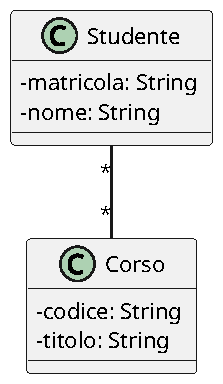
\includegraphics[width=0.2\textwidth]{immagini/cap01_im01.pdf} 
    \caption{Associazione Studente-Corso.}
\end{figure}

L'UML risolve il problema permettendo a un'associazione di avere una propria classe collegata. Questa classe ha un doppio valore: è sia un legame logico tra le istanze, sia un contenitore di attributi.

% Diagramma 2: Classe di associazione (Esame)
% [Codice PlantUML 2]
\begin{figure}[htbp] 
    \centering
    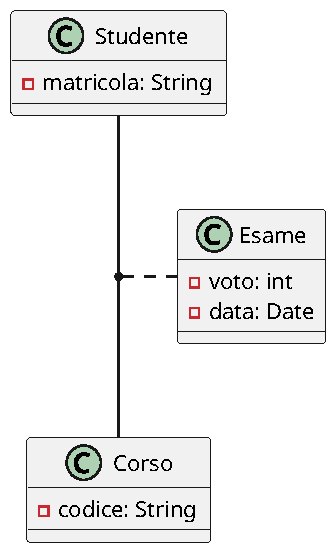
\includegraphics[width=0.3\textwidth]{immagini/cap01_im02.pdf} 
    \caption{Studente-Corso con classe di associazione Esame.}
\end{figure}

Sintatticamente, si rappresenta con un rettangolo di classe collegato alla linea di associazione tramite una \textbf{linea tratteggiata}. Essa eredita implicitamente le "chiavi" di entrambe le classi coinvolte.

In molte fasi di progettazione logica, o per chiarezza di implementazione, la classe di associazione viene "esplicitata" (o reificata). La classe di associazione diventa una classe intermedia a tutti gli effetti, e l'associazione molti-a-molti originale si trasforma in due associazioni uno-a-molti.

% Diagramma 3: Classe esplicitata
% [Codice PlantUML 3]
\begin{figure}[htbp] 
    \centering
    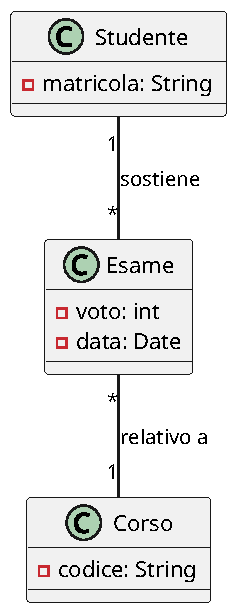
\includegraphics[width=0.2\textwidth]{immagini/cap01_im03.pdf} 
    \caption{Reificazione della classe di associazione Esame.}
    \label{fig:studente_corso}
\end{figure}

L'esplicitazione è spesso necessaria perché molti strumenti di modellazione o linguaggi di programmazione non supportano nativamente il costrutto della classe di associazione. In questo caso, la classe intermedia (es. \texttt{Esame}) funge da "ponte" tra le due entità principali.

\begin{tip}
    La classe di associazione è significativa solo su associazioni \textit{molti-a-molti}, ma occasionalmente si usa anche per altri tipi di associazioni. 
\end{tip}

\subsection{Grado di un'Associazione e Relazioni Ternarie}

Il \textbf{grado} di un'associazione è definito come il numero di classi coinvolte nel legame logico. 
\begin{itemize}
    \item \textbf{Associazioni Binarie (Grado 2):} Collegano due classi. Costituiscono la quasi totalità delle relazioni in un database.
    \item \textbf{Associazioni N-arie (Grado $N \ge 3$):} Collegano tre o più classi contemporaneamente. Il caso più comune è l'associazione \textbf{ternaria}.
\end{itemize}

\medskip

Un'associazione ternaria si rende necessaria quando il legame logico esiste solo se si considerano tre entità simultaneamente; la scomposizione in relazioni binarie separate causerebbe una perdita irreparabile di informazione semantica. In UML si rappresenta graficamente interponendo un \textbf{rombo} tra le linee che collegano le tre classi.

Si consideri, ad esempio, uno scenario di logistica industriale in cui sono coinvolte tre classi: \texttt{Fornitore}, \texttt{Prodotto} e \texttt{Progetto} (cantiere di destinazione). 
L'atto del rifornimento è un evento atomico: il \textit{Fornitore A} fornisce il \textit{Prodotto X} specificamente per il \textit{Progetto Y}. Se provassimo a mappare questo dominio con tre relazioni binarie (\textit{Fornitore-Prodotto}, \textit{Prodotto-Progetto}, \textit{Fornitore-Progetto}), sapremmo quali prodotti vende un fornitore e quali prodotti usa un progetto, ma non sapremmo mai \textbf{quale specifico fornitore ha portato quel determinato prodotto a quel singolo progetto}.

% Diagramma 4: Esempio associazione ternaria
% [Codice PlantUML 4]
\begin{figure}[htbp] 
    \centering
    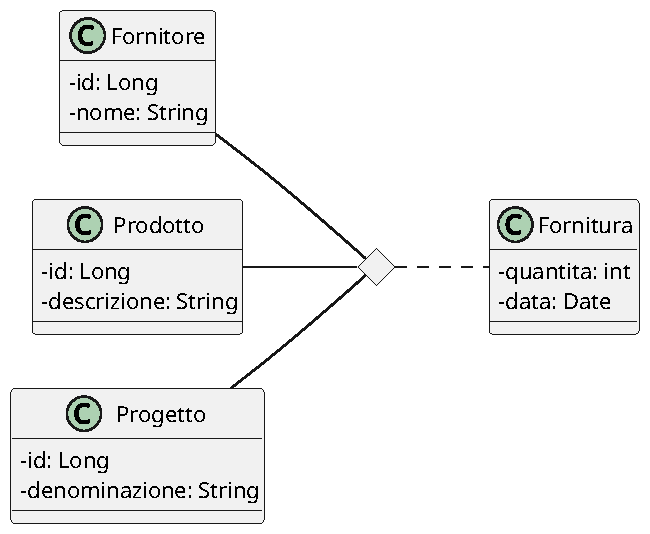
\includegraphics[width=0.5\textwidth]{immagini/cap01_im04.pdf} 
    \caption{Esempio associazione ternaria con classe di associazione.}
    \label{fig:ass_tern}
\end{figure}

\begin{tip}[Interpretazione di una associazione n-aria]
Per comprendere a fondo l'associazione ternaria, si può pensare che una delle tre classi non si colleghi singolarmente alle altre due, ma alla loro \textbf{coppia}. Nel nostro esempio, il \texttt{Progetto} non è legato separatamente a un \texttt{Prodotto} e a un \texttt{Fornitore}, ma è associato stabilmente alla coppia $(Prodotto, Fornitore)$, intesa come specifica combinazione. Analogamente per le altre due classi. 
\end{tip}

Poiché i DBMS relazionali e i framework ORM (come JPA/Hibernate) non supportano le relazioni native a tre vie, si deve \textbf{esplicitare} (o reificare) l'associazione prima dell'implementazione.

La reificazione trasforma il rombo dell'associazione in una classe vera e propria, che chiameremo \texttt{AssegnazioneFornitura}. L'associazione ternaria originale viene così frantumata in tre associazioni binarie distinte di tipo \textbf{1-a-Molti}:
\begin{itemize}
    \item Da \texttt{Fornitore} a \texttt{AssegnazioneFornitura} (Cardinalità \texttt{1} $\rightarrow$ \texttt{*})
    \item Da \texttt{Prodotto} a \texttt{AssegnazioneFornitura} (Cardinalità \texttt{1} $\rightarrow$ \texttt{*})
    \item Da \texttt{Progetto} a \texttt{AssegnazioneFornitura} (Cardinalità \texttt{1} $\rightarrow$ \texttt{*})
\end{itemize}

% Diagramma 5: Reificazione associazione ternaria
% [Codice PlantUML 5]
\begin{figure}[htbp] 
    \centering
    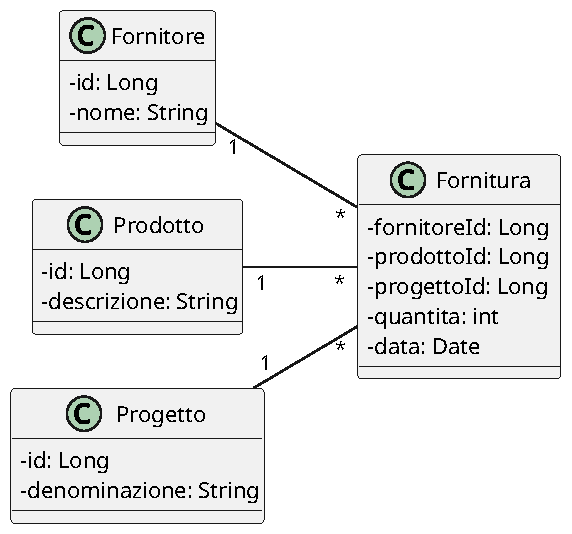
\includegraphics[width=0.5\textwidth]{immagini/cap01_im05.pdf} 
    \caption{Reificazione dell'associazione ternaria.}
    \label{fig:reif_ass_tern}
\end{figure}

Nella realtà, gli eventi n-ari catturano quasi sempre proprietà quantitative. Riprendendo l'esempio precedente, l'atto della fornitura genera intrinsecamente una \textit{quantità} di pezzi consegnati e una \textit{data} di consegna. Questi attributi non appartengono a nessuna delle tre classi isolate, ma alla loro combinazione. In UML si modella una \textbf{Classe di Associazione} (es. \texttt{Fornitura}) collegata tramite una linea tratteggiata al rombo dell'associazione ternaria.

Il processo di esplicitazione in questo scenario è immediato: la classe di associazione \texttt{Fornitura} viene promossa a classe centrale del cluster, inglobando gli attributi \texttt{quantità} e \texttt{data}. Le tre classi originarie si collegano a essa tramite relazioni binarie dirette.

\begin{warningbox}[La trappola delle cardinalità ternarie]
Nelle associazioni ternarie UML, la cardinalità posta vicino a una classe (es. \texttt{Progetto}) indica quante istanze di quella classe possono combinarsi con una \textbf{coppia fissa} di istanze delle altre due classi (\texttt{Fornitore} e \texttt{Prodotto}). Questa logica è controintuitiva e differisce dai diagrammi ER classici (notazione di Chen), inducendo spesso i progettisti in errore. Sostituire subito la ternaria con una classe esplicitata azzera ogni ambiguità interpretativa.
\end{warningbox}

\subsection{Aggregazione e Composizione}

Nello sviluppo dei Class Diagrams, le associazioni standard indicano un legame logico simmetrico. Tuttavia, per modellare scenari in cui esiste un rapporto di possesso o di subordinazione strutturale, l'UML introduce le \textbf{relazioni tutto-parte} (part-whole relationships). Queste si dividono in due varianti fondamentali, distinte in base al vincolo sul ciclo di vita degli oggetti coinvolti: l'aggregazione e la composizione.

L'\textbf{aggregazione} rappresenta una relazione in cui un oggetto ``Tutto'' (aggregante) contiene o colleziona uno o più oggetti ``Parte'' (aggregati), ma questi ultimi mantengono un'esistenza autonoma all'interno del dominio. Si tratta di un legame \textit{``has-a''} ad accoppiamento debole.

\begin{itemize}
    \item \textbf{Sintassi UML:} Si rappresenta graficamente con una linea che termina con un \textbf{rombo vuoto} (bianco) posizionato sul lato della classe ``Tutto''.
    \item \textbf{Ciclo di vita:} La distruzione dell'oggetto aggregante \textbf{non} comporta la distruzione degli oggetti aggregati.
\end{itemize}

\begin{example}[Università e Professore]
Si consideri la classe \texttt{Universita} (il Tutto) e la classe \texttt{Professore} (la Parte). Un'università raccoglie un insieme di docenti. Tuttavia, se l'università dovesse cessare la sua attività, i singoli professori non verrebbero eliminati dal sistema: essi continuerebbero ad esistere come entità autonome e potrebbero essere associati ad altri atenei.
\end{example}

% Diagramma 6: aggregazione
% [Codice PlantUML 6]
\begin{figure}[htbp] 
    \centering
    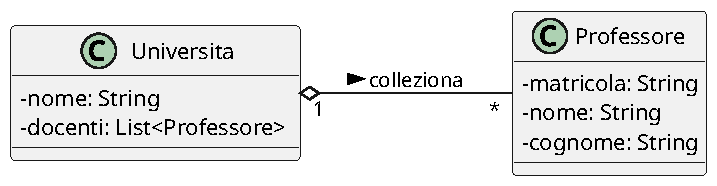
\includegraphics[width=0.5\textwidth]{immagini/cap01_im06.pdf} 
    \caption{Esempio di aggregazione}
\end{figure}



La \textbf{composizione} è una forma di aggregazione più stringente, esclusiva e gerarchica. In questo scenario, l'oggetto ``Parte'' è una componente indissolubile del ``Tutto''. Una parte può appartenere a un solo tutto alla volta e non ha alcuna autonomia esistenziale.

\begin{itemize}
    \item \textbf{Sintassi UML:} Si rappresenta con una linea che termina con un \textbf{rombo pieno} (nero) posizionato sul lato della classe ``Tutto''.
    \item \textbf{Ciclo di vita:} Il ciclo di vita delle parti è totalmente subordinato a quello del tutto. Di conseguenza, la distruzione dell'oggetto composto (Tutto) determina l'istanza di \textbf{distruzione automatica} di tutte le sue parti. La cardinalità dal lato del tutto è rigorosamente \texttt{1} o \texttt{0..1}.
\end{itemize}

\begin{example}[Ordine ed Elemento d'Ordine]
Si consideri un sistema di e-commerce con le classi \texttt{Ordine} (il Tutto) e \texttt{RigaOrdine} (la Parte, che descrive il prodotto e la quantità). Una riga d'ordine ha significato logico solo se contestualizzata all'interno dello specifico acquisto. Se l'utente decide di eliminare l'intero \texttt{Ordine}, il sistema deve rimuovere a cascata tutte le relative istanze di \texttt{RigaOrdine}.
\end{example}

% Diagramma 7: aggregazione
% [Codice PlantUML 7]
\begin{figure}[htbp] 
    \centering
    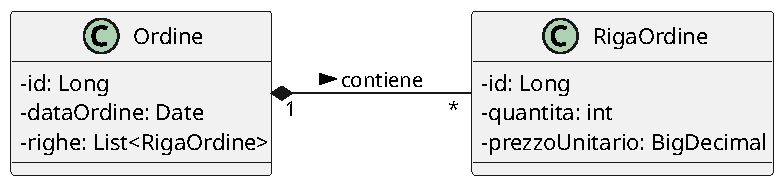
\includegraphics[width=0.5\textwidth]{immagini/cap01_im07.pdf} 
    \caption{Esempio di composizione}
\end{figure}

\begin{dettagli}[]
    L'aggregazione non ha alcuna necessità tecnica stringente: una semplice associazione fa esattamente lo stesso identico lavoro. A livello di tabelle, sia un'associazione generica sia un'aggregazione si tradurranno nello stesso modo, la differenza è puramente semantica e documentale, non implementativa. Alcuni autorevoli ingegneri del software (tra cui Martin Fowler, uno dei padri dell'architettura software moderna) sostengono da anni che l'aggregazione UML sia fondamentalmente inutile perché la linea di demarcazione con l'associazione standard è troppo sfumata e crea più ambiguità che benefici. Fowler la definisce ironicamente "un effetto placebo grafico".

    Il caso della composizione è invece più significativo, perché il diagramma fornisce un'informazione in più: la parte non può esistere senza il tutto. 
\end{dettagli}

\subsection{Generalizzazioni/Specializzazioni}

L'ereditarietà modella una relazione di tipo \textit{``IS-A''} (è-un) tra una classe più generale, detta \textbf{Generalizzazione} (o Superclasse, per analogia con i contesti OOP), e una o più classi più specifiche, dette \textbf{Specializzazioni} (o Sottoclassi). 

Le specializzazioni ereditano automaticamente tutti gli attributi, i ruoli e le associazioni della generalizzazione, senza necessità di ridefinirli, e possono estendere il modello introducendo attributi o associazioni propri.

\textbf{Sintassi UML:} Si rappresenta graficamente con una linea che termina con una \textbf{freccia con la punta triangolare vuota} rivolta verso la generalizzazione.

% Diagramma 8: aggregazione
% [Codice PlantUML 8]
\begin{figure}[htbp] 
    \centering
    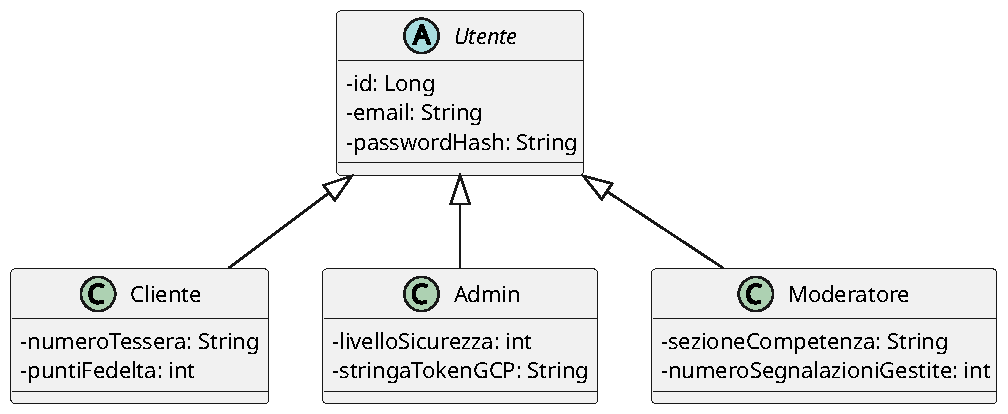
\includegraphics[width=0.7\textwidth]{immagini/cap01_im08.pdf} 
    \caption{Esempio di ereditarietà}
\end{figure}

È fondamentale comprendere che \textbf{l'ereditarietà non esiste nel modello relazionale delle basi di dati} (o almeno, non secondo il modello relazionale dei dati che noi studieremo). I database relazionali non possiedono strutture gerarchiche native; essi conoscono esclusivamente il concetto di tabella (relazione), che è per sua natura una struttura ``piatta'' e bidimensionale. 

La generalizzazione appartiene quindi in modo esclusivo al livello della \textbf{progettazione concettuale}. In questa fase, lo scopo del Class Diagram è modellare il dominio reale nel modo più fedele e naturale possibile, catturandone la semantica e i vincoli logici (ovvero i rapporti di sotto-tipo/sopra-tipo) ed eliminando qualsiasi vincolo tecnologico. Il problema di come ``appiattire'' questa gerarchia per adattarla a un database relazionale sarà l'obiettivo centrale della successiva fase di progettazione logica.

\medskip

Una generalizzazione può essere classificata combinando due tipi di vincoli ortogonali, utili a descrivere la natura delle istanze nel dominio reale:

\begin{enumerate}
    \item \textbf{Completezza (Totale vs Parziale):}
    \begin{itemize}
        \item \textbf{Totale (Complete):} Ogni istanza della superclasse deve obbligatoriamente appartenere ad almeno una delle subclassi. Non esistono elementi ``generici'' (corrisponde al concetto di \textit{Classe Astratta} in OOP).
        \item \textbf{Parziale (Incomplete):} Un'istanza della superclasse può esistere senza dover per forza appartenere a una delle subclassi catalogate.
    \end{itemize}
    \item \textbf{Disgiunzione (Disgiunta vs Sovrapposta):}
    \begin{itemize}
        \item \textbf{Disgiunta (Disjoint):} Un'istanza della superclasse può appartenere al massimo a \textbf{una sola} delle subclassi. Le sottoclassi sono mutuamente esclusive.
        \item \textbf{Sovrapposta (Overlapping):} Una singola istanza della superclasse può appartenere contemporaneamente a più subclassi distinte.
    \end{itemize}
\end{enumerate}

\medskip

Ci sono dunque quattro combinazioni possibili. Nel diagramma UML, i vincoli della generalizzazione si indicano inserendo un'etichetta testuale racchiusa tra parentesi graffe (\textit{Generalization Set}) in prossimità delle linee di ereditarietà, specificando la coppia di proprietà (es: \texttt{\{complete, overlapping\}}).

\begin{example}[Esempi di Vincoli]
Si considerino i seguenti scenari aziendali:
\begin{itemize}
    \item \textbf{Totale / Disgiunta:} La superclasse \texttt{ContoBancario} ha come subclassi \\ \texttt{ContoCorrente} e \texttt{ContoDeposito}. Un conto deve essere obbligatoriamente di un tipo o dell'altro, e non può essere entrambe le cose contemporaneamente.
    \item \textbf{Parziale / Sovrapposta:} La superclasse \texttt{Persona} ha come subclassi \texttt{Studente} e \texttt{Dipendente}. All'interno dell'anagrafica universitaria, una persona può essere solo un cittadino esterno (parziale), oppure può essere contemporaneamente uno studente che lavora per l'ateneo (sovrapposta).
\end{itemize}
\end{example}

\section{La Documentazione di Supporto: I Dizionari dei Dati}

Il Class Diagram, pur essendo uno strumento visivo formidabile, non è espressivamente sufficiente a catturare l'intera semantica di un dominio applicativo. Elementi come il significato preciso di un attributo, il contesto d'uso di un'associazione o le regole aziendali complesse (\textit{Business Rules}) non possono essere espressi tramite nodi e archi. 

La progettazione concettuale si completa quindi attraverso i \textbf{Dizionari dei Dati}, estensioni testuali strutturate che definiscono formalmente ogni componente dello schema concettuale. Questi documenti rappresentano la specifica dei requisiti su cui si baserà lo sviluppo dello strato di persistenza e della logica di business.

\medskip

I dizionari dei dati sono: 
\begin{itemize}
    \item \textbf{Dizionario delle Classi}: descrive in modo univoco ogni entità del sistema. Si presenta come una tabella in cui ogni riga rappresenta una classe. Per ogni classe vengono forniti il nome (prima colonna), una descrizione in linguaggio naturale per evitare ambiguità terminologiche (seconda colonna), nome, tipo e descrizione di ciascun attributo (terza colonna).
    \item \textbf{Dizionario delle Associazioni}: si presenta come una tabella analoga alla precedente, in cui ogni riga rappresenta un'associazione. Per ogni associazione vengono forniti il nome (prima colonna), descrizione (seconda colonna), le classi coinvolte con ruolo, molteplicità e descrizione (terza colonna). 
    \item \textbf{Dizionario dei Vincoli}: è il documento più critico. I \textbf{Vincoli di Integrità Esogeni} (o regole di business) sono restrizioni sul dominio dei dati che \textbf{non possono} essere espresse graficamente nel Class Diagram tramite la normale sintassi UML. Mentre una cardinalità \texttt{1..*} esprime un vincolo strutturale grafico, una regola del tipo \textit{``Un cliente non può effettuare un ordine se il suo account è sospeso''} non ha un simbolo UML dedicato. Viene quindi codificata nel dizionario dei vincoli in linguaggio naturale o tramite espressioni logico-matematiche formali (come l'OCL - \textit{Object Constraint Language}). Si presenta come una tabella a due colonne in cui ogni riga rappresenta un vincolo, nella prima colonna si inserisce il nome del vincolo oppure un suo identificatore univoco (es. \texttt{BR} - Business Rule), nella seconda colonna la sua descrizione in linguaggio naturale. 
\end{itemize}

\begin{example}[Catalogo dei Vincoli d'Integrità]
\begin{description}
    \item 
    \item[\texttt{BR01} (Coerenza Temporale):] La data di spedizione di un \texttt{Ordine} deve essere strettamente successiva o uguale alla sua data di creazione.
    \item[\texttt{BR02} (Integrità Finanziaria):] L'attributo \texttt{totale} di un \texttt{Ordine} deve essere matematicamente pari alla sommatoria del prodotto tra \texttt{quantita} e \texttt{prezzoUnitario} di tutte le istanze di \texttt{RigaOrdine} a esso collegate.
    \item[\texttt{BR03} (Regola di Business):] Un \texttt{Utente} con ruolo \texttt{Admin} non può associare a sé stesso un'istanza di \texttt{Ordine} in veste di \texttt{acquirente}.
\end{description}
\end{example}

\begin{bestpractice}[]
    Nel dizionario dei vincoli non vanno inseriti vincoli che sono già espressi nel class diagram. 

    I vincoli devono garantire la qualità interna dei dati nella base di dati. 
\end{bestpractice}





\chapter{Modello Relazionale e Progettazione Logica}

\section{Introduzione}

Il passaggio dalla progettazione concettuale alla progettazione logica rappresenta la transizione dal \textit{cosa} deve essere rappresentato al \textit{come} organizzare concretamente i dati all'interno di un sistema di gestione di basi di dati (DBMS). Questo processo richiede l'adozione di uno specifico \textbf{modello dei dati}.

Sebbene la storia dell'informatica abbia visto l'evoluzione di diversi paradigmi — come il modello gerarchico, quello reticolare e quello orientato agli oggetti —, la nostra trattazione si concentrerà sul \textbf{modello relazionale}, che costituisce lo standard industriale prevalente. Vale la pena notare che i DBMS moderni più diffusi (come PostgreSQL e Oracle) adottano un'evoluzione di questo approccio, denominata \textbf{modello relazionale a oggetti}, la quale estende le fondamenta del modello relazionale puro integrando costrutti tipici del paradigma OOP.

\medskip

Uno dei principali vantaggi nell'aver adottato i \textbf{Class Diagrams UML} nella fase concettuale risiede nella loro assoluta indipendenza tecnologica: essi si adattano teoricamente a qualunque modello logico finale. Di contro, questa spiccata espressività introduce un inevitabile \textbf{disallineamento semantico} (\textit{impedance mismatch}) quando l'obiettivo è la traduzione in uno schema relazionale puro. 

Nel passaggio alla progettazione logica relazionale, le principali sfide strutturali da affrontare saranno dettate dai rigidi vincoli di atomicità e piattezza del dato tipici delle tabelle:
\begin{itemize}
    \item \textbf{Attributi strutturati:} Il modello relazionale esige che i valori degli attributi siano atomici e non strutturati. Non è quindi possibile nidificare record, oggetti o tipi di dato complessi all'interno di una colonna.
    \item \textbf{Attributi a valore multiplo (multivalore):} Ogni cella di una tabella relazionale può contenere esclusivamente un singolo valore atomico, vietando l'uso nativo di collezioni, array, liste o set all'interno di un singolo attributo.
    \item \textbf{Assenza di ereditarietà:} Il modello relazionale puro non supporta nativamente le gerarchie di generalizzazione-specializzazione, costringendo il progettista ad applicare strategie di ``appiattimento'' o di scomposizione strutturale.
\end{itemize}


\section{Concetti Fondamentali}

Il \textbf{modello relazionale} si basa sul concetto matematico di relazione. Questo modello rappresenta la struttura logica e piatta su cui verranno mappati i dati dell'applicazione. Per formalizzare rigorosamente il modello, è necessario definire i suoi tre componenti atomici: i domini, lo schema e la relazione stessa.

\medskip

Un \textbf{dominio} (indicato con $D$) è un insieme di valori atomici, ovvero non ulteriormente scomponibili. 
Ogni dominio è caratterizzato da un nome e da un tipo di dato (es: \texttt{int, varchar, date}).
\begin{observation}[Il Tipo di Dato come Dominio Implicito]
Nella transizione dalla teoria all'ingegneria del software, il \textbf{tipo di dato} (es. \texttt{int}, \texttt{varchar}, \texttt{date}) definisce l'insieme universo di partenza, agendo come \textbf{dominio massimo implicito} dell'attributo. 

Eventuali restrizioni logiche (come un \textit{range} di valori validi per un voto universitario o un'età) si configurano come un \textbf{sottoinsieme} di tale dominio base. Vedremo in seguito come vengono implementate limitazioni specifiche. 
\end{observation}

\medskip

Uno \textbf{schema relazionale} (o schema di tabella) definisce la struttura logica dei dati. Esso è costituito da un nome $R$ e da un insieme di attributi $A_1, A_2, \dots, A_n$, a ciascuno dei quali è associato un dominio $D_i$, che denoteremo anche con $dom(A_i)$.

Lo schema viene denotato formalmente come:
$$R(A_1: D_1, A_2: D_2, \dots, A_n: D_n)$$

Lo schema relazionale corrisponde dunque esattamente al concetto di \textbf{Classe}. Esso definisce la struttura dei dati, i nomi dei campi e i rispettivi tipi, agendo come un ``blueprint'' statico.

Matematicamente, date le premesse precedenti, definiamo il dominio totale dello schema come il prodotto cartesiano dei domini dei singoli attributi:
$$D_{tot} = D_1 \times D_2 \times \dots \times D_n$$

\medskip

Una \textbf{relazione} $r$ sullo schema $R$ è un sottoinsieme finito del prodotto cartesiano dei domini degli attributi:
$$r \subseteq D_1 \times D_2 \times \dots \times D_n$$

Gli elementi che compongono questo sottoinsieme sono detti \textbf{tuple} (o n-uple). Una tupla è un vettore di valori $(v_1, v_2, \dots, v_n)$ tale che ogni $v_i \in D_i$.

\begin{tip}[]
La corrispondenza con OOP è la seguente:
\begin{itemize}
    \item Una \textbf{Tupla} corrisponde al singolo \textbf{Oggetto} (una istanza della classe contenente dati reali).
    \item La \textbf{Relazione} corrisponde all'insieme di tutti gli oggetti di quella classe \textbf{attualmente persistiti} nel database in un determinato istante temporale (lo stato corrente della tabella).
\end{itemize}
\end{tip}

\begin{example}[Formalizzazione di un'Anagrafica]
Definiamo lo schema relazionale per la classe \texttt{Studente}:
$$STUDENTE(\text{matricola}: \text{String}, \text{ nome}: \text{String}, \text{ eta}: \text{Integer})$$

Il prodotto cartesiano di questi tre domini genererebbe infinite combinazioni (comprese matricole inesistenti accoppiate a nomi casuali ed età assurde). 

La \textbf{relazione} $r(\text{STUDENTE})$ conterrà invece solo le tuple degli studenti reali inseriti nel sistema:
$$r = \{(\text{'654321'}, \text{'Giovanni'}, 22), (\text{'123456'}, \text{'Mario'}, 24)\}$$
\end{example}

\begin{observation}
    È significativo evidenziare che una relazione \textit{è un insieme}, dunque \textit{non ammette duplicati e non rappresenta una struttura ordinata}. 
\end{observation}

\begin{tip}[In sintesi:]
Nel passaggio dalla progettazione concettuale alla modellazione logica, i concetti del paradigma orientato agli oggetti (\textit{OOP}) e del Class Diagram si traducono come segue:

\begin{itemize}
    \item \textbf{Classi $\rightarrow$ Schemi Relazionali:} Le classi si traducono in schemi di relazione, identificati da un nome (corrispondente al nome della classe) e da un insieme di attributi.
    \item \textbf{Attributi $\rightarrow$ Domini:} A ciascun attributo dello schema è associato un \textbf{dominio}, ovvero l'insieme di tutti i possibili valori atomici che quell'attributo può assumere (equivalente al tipo di dato in programmazione).
    \item \textbf{Istanze $\rightarrow$ Relazione (Stato):} Una \textbf{relazione} è un sottoinsieme discreto e finito del dominio totale (il prodotto cartesiano di tutti i singoli domini). Essa rappresenta l'insieme delle tuple (istanze o oggetti) effettivamente memorizzate e persistite nel sistema in un dato momento temporale.
\end{itemize}
\end{tip}

% Consideriamo ora, nel class diagram, l'associazione studente-esame (uno a molti). A partire da una istanza di esame, per risalire allo studente che ha sostenuto quell'esame uso la chiave esterna matricola, da cui risalgo all'identificatore dello studente (matr, chiave primaria di STUDENTE).

% Da sottolineare quando si vanno rendere le associazioni molti a molti:

% sono problematiche perché il modello relazionale mi impone un valore unico per ciascun attributo, quindi non posso usare lo stesso metodo che uso per le associazioni uno a molti. 

% Il metodo per le associazioni molti a molti è del tutto generale ed in teoria si potrebbe usare per tutti i tipi di associazione; tuttavia questo metodo si usa solo dove strettamente necessario, perché ha un costo. 

\section{Le Chiavi}

Fino ad ora abbiamo analizzato come tradurre classi e attributi del Class Diagram nel modello relazionale, lasciando in sospeso la traduzione delle associazioni. Per poter modellare le relazioni tra tabelle, è prima necessario introdurre il concetto di chiave.

\medskip

Sia $R(A_1, A_2, \dots, A_n)$ uno schema di relazione. Un sottoinsieme di attributi $SK \subseteq \{A_1, A_2, \dots, A_n\}$ si definisce \textbf{superchiave} se i suoi valori identificano in modo univoco ogni singola tupla all'interno di qualsiasi istanza valida della relazione. 

\begin{example}[Superchiavi di un'Anagrafica]
Si consideri lo schema: 
$$\texttt{STUDENTE}({\text{CF}}, \text{ matricola}, \text{ nome}, \text{ cognome}, \text{ dataNascita})$$
I singoletti $\{\text{CF}\}$ e $\{\text{matricola}\}$ sono superchiavi. Di conseguenza, \textbf{qualsiasi sottoinsieme che li contenga} (es: $\{\text{CF}, \text{nome}\}$ o $\{\text{matricola}, \text{cognome}\}$) è a sua volta una superchiave.
\end{example}

\begin{observation}[Ipotesi di Esistenza]
Nella fase di progettazione concettuale si assume l'ipotesi che ogni istanza di una classe sia distinguibile dalle altre. Questa proprietà ci garantisce che \textbf{esiste sempre almeno una superchiave} per ogni schema relazionale: nella peggiore delle ipotesi (assenza di identificatori naturali), la superchiave coinciderà con l'insieme di tutti gli attributi dello schema.
\end{observation}

\medskip

Un sottoinsieme di attributi $K$ è una \textbf{chiave candidata} se è una \textbf{superchiave minimale}. Dire che una superchiave è \textit{minimale} significa che è \textbf{irriducibile}: eliminando un qualsiasi attributo da $K$, l'insieme rimanente perde la proprietà di univocità e cessa di essere una superchiave. 

Questo \textbf{non} significa che debba avere il numero minimo di attributi in assoluto (cardinalità minima). Se nello schema coesistono una superchiave irriducibile di cardinalità 1 e una di cardinalità 2, sono entrambe, con pari dignità, chiavi candidate.

È evidente che una superchiave composta da un unico attributo (un singoletto) è di fatto e necessariamente una chiave candidata.

\begin{example}[Chiave Candidata Composta]
Si consideri lo schema che mappa la classe degli esami universitari:
$$\texttt{ESAME}(\text{matricola}, \text{ corso}, \text{ voto}, \text{ data})$$
In questo scenario, il sottoinsieme $\{\text{matricola}, \text{corso}\}$ rappresenta una chiave candidata (di fatto, è l'unica chiave candidata in questo caso). Essa è minimale perché se eliminassimo \texttt{corso}, la sola \texttt{matricola} non garantirebbe l'univocità (uno studente può sostenere più esami); viceversa, eliminando \texttt{matricola}, il solo \texttt{corso} conterrebbe i voti di tutti gli studenti.
\end{example}

\medskip

Poiché in uno schema relazionale possono coesistere più chiavi candidate, il progettista deve sceglierne una da eleggere come identificatore ufficiale delle tuple. La chiave candidata scelta prende il nome di \textbf{Chiave Primaria} (\textit{Primary Key} - PK).

La selezione della chiave primaria è una decisione puramente ingegneristica e architetturale. Nello schema relazionale scritto, la chiave primaria si indica \textbf{sottolineando} gli attributi che la compongono.

\begin{example}[Scelta della PK]
Riprendendo lo schema \texttt{STUDENTE}, le chiavi candidate sono \texttt{CF} e \texttt{matricola}. Sceglieremo come chiave primaria la \texttt{matricola}:
$$\texttt{STUDENTE}(\text{CF}, \underline{\text{matricola}}, \text{nome}, \text{cognome})$$
\end{example}

\medskip

La \textbf{Chiave Esterna} (\textit{Foreign Key} - FK) è lo strumento fondamentale del modello relazionale per tradurre le associazioni.

Siano $R_1$ e $R_2$ due schemi relazionali (non necessariamente distinti). Un insieme di attributi $FK$ di $R_1$ è una chiave esterna che punta a $R_2$ se:
\begin{enumerate}
    \item Gli attributi in $FK$ sono in corrispondenza biunivoca con gli attributi che compongono la \textbf{chiave primaria} ($PK$) di $R_2$.
    \item I domini degli attributi corrispondenti sono identici ($dom(FK_i) = dom(PK_i)$).
\end{enumerate}

\medskip

Il vincolo impone che per ogni tupla $t_1$ nell'istanza corrente di $R_1$, il valore di $t_1[FK]$ deve essere nullo (\texttt{NULL}), oppure coincidere esattamente con il valore $t_2[PK]$ di \textbf{una tupla} $t_2$ \textbf{attualmente esistente} nell'istanza di $R_2$.

Nello schema testuale, la presenza di una chiave esterna si denota convenzionalmente con una \textbf{doppia sottolineatura}.

\section{Traduzione delle Associazioni}

\subsection{Associazioni 1 a 1}

Un'associazione \textbf{1 a 1} tra due classi $A$ e $B$ indica che a un'istanza di $A$ corrisponde al massimo un'istanza di $B$, e viceversa. 
Nel modello relazionale, questo legame si traduce introducendo una \textbf{Chiave Esterna (FK)} in uno dei due schemi che punta alla Chiave Primaria (PK) dell'altro.

\begin{example}[Associazione esattamente 1 a 1]
Si consideri un'associazione in cui la partecipazione è rigida e obbligatoria per entrambe le classi (1..1 $\leftrightarrow$ 1..1), ad esempio tra l'entità \texttt{STUDENTE(matricola, nome, cognome)} e il suo \texttt{FASCICOLO(codice, dataCreazione)}. Ogni studente possiede esattamente un fascicolo e ogni fascicolo appartiene esattamente a uno studente.
Traduciamo il modello aggiungendo la chiave esterna nello schema del fascicolo:
\begin{itemize}
    \item $\texttt{STUDENTE}(\underline{\text{matricola}}, \text{ nome}, \text{ cognome})$
    \item $\texttt{FASCICOLO}(\underline{\text{codice}}, \text{ dataCreazione}, \underline{\underline{\text{ matricolaStudente}}})$
\end{itemize}
\end{example}

Affinché la relazione rimanga rigorosamente 1 a 1, non è sufficiente definire la chiave esterna. Se ci limitassimo a questo, la tabella che ospita la FK potrebbe avere più tuple che puntano alla stessa PK della tabella bersaglio, trasformando di fatto la relazione in una 1 a N.

Riprendendo l'esempio precedente, se l'attributo \texttt{studente} nello schema \texttt{FASCICOLO} fosse definito unicamente come chiave esterna, nulla impedirebbe al database di registrare due tuple distinte di fascicoli (es. codice \texttt{'F01'} e \texttt{'F02'}) aventi entrambe il valore \texttt{studente = '12345'}. Questo corromperebbe la semantica concettuale, asserendo che la matricola 12345 possiede \textit{molti} fascicoli.

Per garantire la biunivocità dell'associazione, è obbligatorio imporre un \textbf{vincolo di univocità} sugli attributi che compongono la chiave esterna.
Matematicamente, se lo schema $R_1$ contiene la chiave esterna $FK$ verso $R_2$, deve valere che per ogni coppia di tuple distinte $t_x, t_y \in r(R_1)$:
$$t_x[FK] \neq t_y[FK] \quad \text{(escludendo i valori NULL)}$$

\begin{dettagli}[Perché usare una sola Chiave Esterna?]
Vista la forte simmetria di un'associazione 1 a 1, potrebbe sorgere spontaneo il dubbio: perché non posizionare una chiave esterna in \textit{entrambi} gli schemi (es. aggiungere \texttt{fascicolo} dentro \texttt{STUDENTE} e \texttt{studente} dentro \texttt{FASCICOLO})? 
La teoria relazionale esclude questa pratica per tre ragioni fondamentali:
\begin{enumerate}
    \item \textbf{Ridondanza e Rischio di Anomalie:} Il legame logico verrebbe salvato due volte. Se per errore un sistema aggiornasse un lato senza allineare l'altro (es. lo Studente punta al Fascicolo A, ma il Fascicolo A punta a un altro Studente), il database entrerebbe in uno stato incoerente.
    \item \textbf{Bidirezionalità Intrinseca:} Come già stabilito, la presenza di una singola chiave esterna è matematicamente sufficiente per stabilire un'uguaglianza logica tra le tuple. Il motore del database può navigare il legame in entrambe le direzioni senza bisogno di puntatori doppi.
    \item \textbf{Dipendenza Circolare (Deadlock di Inserimento):} Poiché in questo esempio la partecipazione è obbligatoria da ambo i lati, le rispettive chiavi esterne dovrebbero avere un vincolo \texttt{NOT NULL}. Tuttavia, questo creerebbe un paradosso logico: non si potrebbe inserire uno studente nel database perché manca il suo fascicolo, e non si potrebbe inserire il fascicolo perché manca lo studente a cui associarlo. Inserire la chiave esterna in un solo schema spezza questo circolo vizioso.
\end{enumerate}
\end{dettagli}

\begin{observation}
    In alcuni casi estremi di forte coesione, le due tabelle possono persino essere fuse in un unico schema relazionale. Approfondiremo questo aspetto nel prossimo paragrafo. 
\end{observation}

Nell'esempio precedente si aveva una situazione di relazione esattamente 1 a 1 e la scelta dello schema in cui inserire la chiave esterna era indifferente. In altri casi, la scelta di quale delle due tabelle debba ospitare la FK dipende dalle \textbf{cardinalità minime} (l'opzionalità o obbligatorietà dell'associazione): se la classe $A$ partecipa in modo opzionale (0..1) e la classe $B$ in modo obbligatorio (1..1), la chiave esterna \textbf{deve essere inserita nello schema $B$}. In questo modo, la $FK$ in $B$ potrà essere dichiarata \texttt{NOT NULL} (vincolo di esistenza garantito). Se la mettessimo in $A$, saremmo costretti ad ammettere valori \texttt{NULL} per le istanze di $A$ che non partecipano all'associazione, sprecando spazio e riducendo l'eleganza relazionale.

\begin{example}[Direzione di un Dipartimento]
Si consideri l'associazione 1 a 1 tra \texttt{Professore} (0..1) e \texttt{Dipartimento} (1..1): un professore può dirigere al massimo un dipartimento, ma un dipartimento deve avere esattamente un direttore.

Seguendo la regola, posizioniamo la chiave esterna nel \texttt{Dipartimento}:
\begin{itemize}
    \item $\texttt{PROFESSORE}(\underline{\text{codiceDocente}}, \text{nome}, \text{cognome})$
    \item $\texttt{DIPARTIMENTO}(\underline{\text{codice}}, \text{nome}, \underline{\underline{\text{codiceDirettore}}})$
\end{itemize}

\medskip

Vincoli su \texttt{DIPARTIMENTO.codiceDirettore}:
\begin{itemize}
    \item \textbf{Foreign Key:} punta a \texttt{PROFESSORE.codiceDocente}
    \item \textbf{UNIQUE:} per garantire che lo stesso professore non diriga due dipartimenti (vincolo 1:1).
    \item \textbf{NOT NULL:} per garantire che ogni dipartimento abbia un direttore (cardinalità minima 1).
\end{itemize}
\end{example}

\begin{dettagli}[Controllo Applicativo vs Vincolo Strutturale (UNIQUE)]
In alcuni contesti didattici o in framework di sviluppo specifici, è possibile omettere la dichiarazione esplicita del vincolo \texttt{UNIQUE} per le associazioni 1 a 1. 

In questi scenari, si assume un'ipotesi di \textbf{coerenza applicativa}: si dà per scontato che sia la logica del software sovrastante (es. i controlli nel codice backend) a impedire l'inserimento di tuple multiple, in accordo con la natura del dominio (``non può mai capitare che l'entità sia associata a molti'').

Tuttavia, dal punto di vista della solidità ingegneristica e dell'integrità fisica dei dati (\textit{defensive programming}), l'omissione del vincolo \texttt{UNIQUE} rende il database strutturalmente identico a un'associazione 1 a Molti. Fissare il vincolo a livello di DBMS rimane la pratica raccomandata per garantire che i dati non vengano mai corrotti, indipendentemente da eventuali bug del software applicativo.
\end{dettagli}

\subsection{Associazioni 1 a Molti (1:N)}

Nel modello relazionale, questa associazione si traduce secondo una regola fissa e inderogabile, dettata dal vincolo di atomicità degli attributi (assenza di attributi multivalore): la \textbf{Chiave Esterna (FK) deve essere sempre inserita nello schema dal lato ``Molti'' ($B$)}, e punterà alla Chiave Primaria (PK) dello schema dal lato ``Uno'' ($A$).

A differenza dell'associazione 1 a 1, in questo caso \textbf{non} si deve applicare alcun vincolo di univocità (\texttt{UNIQUE}) sulla chiave esterna. È infatti intrinseco nella natura dell'associazione 1:N che più tuple della relazione $B$ possano possedere lo stesso valore per l'attributo FK, puntando così alla medesima istanza di $A$.

\begin{example}[Impiegati in un Dipartimento]
Si consideri l'associazione tra \texttt{Dipartimento} (1) e \texttt{Impiegato} (N). Un dipartimento ospita molti impiegati, ma un impiegato afferisce a un solo dipartimento.
La chiave esterna viene posizionata nello schema \texttt{IMPIEGATO}:

\begin{itemize}
    \item $\texttt{DIPARTIMENTO}(\underline{\text{codice}}, \text{nome}, \text{sede})$
    \item $\texttt{IMPIEGATO}(\underline{\text{matricola}}, \text{nome}, \text{cognome}, \underline{\underline{\text{codiceDipartimento}}})$
\end{itemize}
\end{example}

\begin{observation}[Monodirezionalità Apparente]
Anche in questo caso, la posizione fisica della chiave esterna genera una \textit{monodirezionalità apparente}. Guardando lo schema, sembra che un impiegato "conosca" il proprio dipartimento, ma che il dipartimento sia ignaro dei propri impiegati (poiché non ha attributi che li referenziano). 

Come già chiarito, questa è solo un'illusione strutturale: l'informazione è conservata intatta dalla logica dei valori. Il database è sempre in grado di ricavare l'elenco degli impiegati di uno specifico dipartimento, semplicemente interrogando la tabella \texttt{IMPIEGATO} e filtrando le tuple che possiedono quel determinato \texttt{codiceDipartimento}.
\end{observation}

\subsection{Associazioni Molti a Molti (N:N)}

Nei casi precedenti (1:1 e 1:N), la traduzione avveniva inserendo una chiave esterna direttamente in uno dei due schemi coinvolti. 
Se provassimo ad applicare questa logica a un'associazione N:N, violeremmo il vincolo fondamentale del modello relazionale:
\begin{itemize}
    \item Inserire la chiave esterna di \texttt{CORSO} nello schema \texttt{STUDENTE} costringerebbe una tupla studente a contenere un attributo \textbf{multivalore} (una lista di codici di corsi).
    \item Viceversa, inserire la chiave esterna di \texttt{STUDENTE} in \texttt{CORSO} creerebbe una lista di matricole dentro la tupla del corso.
\end{itemize}
Poiché il modello relazionale ammette esclusivamente valori atomici, l'uso di chiavi esterne dirette è matematicamente impossibile.

\medskip

Per tradurre un'associazione Molti a Molti, la teoria relazionale impone la creazione di un \textbf{terzo schema di relazione autonomo}, comunemente chiamato \textit{tabella di giunzione}, \textit{tabella ponte} o \textit{relazione associativa}.

Questa nuova tabella conterrà esclusivamente (almeno nella sua forma base) le chiavi esterne che puntano alle chiavi primarie dei due schemi originari. La \textbf{Chiave Primaria} di questa nuova tabella sarà composta dall'unione delle due chiavi esterne (chiave primaria composta).

\begin{example}[Studenti e Corsi]
Si consideri l'associazione N:N tra \texttt{STUDENTE} e \texttt{CORSO}.
Creiamo la tabella ponte \texttt{FREQUENZA}:

\begin{itemize}
    \item $\texttt{STUDENTE}(\underline{\text{matricola}}, \text{nome})$
    \item $\texttt{CORSO}(\underline{\text{codice}}, \text{titolo}, \text{cfu})$
    \item $\texttt{FREQUENZA}(\underline{\underline{\text{matricolaStudente}}}, \underline{\underline{\text{codiceCorso}}})$
\end{itemize}

\medskip

Vincoli sulla tabella \texttt{FREQUENZA}:
\begin{itemize}
    \item \textbf{Primary Key:} È composta dalla coppia (\texttt{matricolaStudente}, \texttt{codiceCorso}). Questo garantisce che uno studente non possa essere iscritto due volte allo stesso identico corso.
    \item \textbf{Foreign Key 1:} \texttt{matricolaStudente} punta a \texttt{STUDENTE.matricola}.
    \item \textbf{Foreign Key 2:} \texttt{codiceCorso} punta a \texttt{CORSO.codice}.
\end{itemize}
\end{example}

\begin{observation}[Delegazione della Complessità]
Dal punto di vista della progettazione (struttura statica), il pattern della tabella di giunzione rende la risoluzione delle associazioni N:N un processo banale e standardizzato.
La reale complessità viene delegata alla fase operativa (interrogazione dei dati). Per estrarre, ad esempio, i nomi degli studenti e i titoli dei corsi da loro frequentati, il DBMS dovrà eseguire computazionalmente onerosi \textbf{JOIN multipli}, attraversando la tabella ponte per ricongiungere i dati disaccoppiati.

È chiaro che questo metodo per rendere le associazioni è del tutto generale e, in teoria, potrebbe essere usato per tutti i tipi di associazione; tuttavia, si tratta ovviamente di una cattiva pratica in virtù del costo computazionale che è stato appena discusso. 
\end{observation}

\subsubsection*{Classi di Associazione}

Nel modellamento concettuale tramite Class Diagram UML, capita frequentemente che un'associazione molti a molti possieda a sua volta degli attributi (formalizzati tramite una \textbf{Classe di Associazione}). Un esempio tipico è la relazione di superamento di un esame tra uno studente e un corso, la quale porta con sé attributi come il \textit{voto}, la \textit{data} e la \textit{lode}.

La traduzione di questo costrutto nel modello relazionale segue fedelmente la regola dello schema ponte vista in precedenza. Gli attributi propri dell'associazione vengono semplicemente inseriti come \textbf{colonne aggiuntive all'interno della tabella di giunzione}.

\begin{example}[Mappatura della Classe di Associazione Esame]
Estendiamo l'esempio precedente trasformando lo schema ponte \texttt{FREQUENZA} in uno schema \texttt{ESAME} che ospiti anche i dati del superamento del corso:

\begin{itemize}
    \item $\texttt{STUDENTE}(\underline{\text{matricola}}, \text{nome}, \text{cognome})$
    \item $\texttt{CORSO}(\underline{\text{codice}}, \text{titolo}, \text{cfu})$
    \item $\texttt{ESAME}(\underline{\underline{\text{matricolaStudente}}}, \underline{\underline{\text{codiceCorso}}}, \text{voto}, \text{data}, \text{lode})$
\end{itemize}

\medskip

Nello schema \texttt{ESAME}, la chiave primaria rimane la coppia composta (matricolaStudente, codiceCorso), il che modella il vincolo per cui uno studente può registrare al massimo un voto per un determinato corso. Gli attributi \texttt{voto}, \texttt{data} e \texttt{lode} diventano attributi non chiave della tabella di giunzione.
\end{example}

\subsubsection{Associazioni n-arie}

La logica della tabella di giunzione, introdotta per le associazioni binarie Molti a Molti, scala in modo naturale e identico per le \textbf{associazioni n-arie} (con $n > 2$). 

Quando nel diagramma concettuale un'associazione coinvolge tre o più classi (ad esempio un'associazione ternaria), la traduzione nel modello relazionale richiede la creazione di un unico \textbf{schema ponte} dedicato. Questo schema assolverà il compito di legare tutte le entità simultaneamente e conterrà:
\begin{itemize}
    \item Una \textbf{Chiave Esterna (FK)} per ciascuna delle $n$ entità partecipanti, che punta alla rispettiva chiave primaria.
    \item Una \textbf{Chiave Primaria (PK) composta} dall'unione di tutte le chiavi esterne coinvolte (salvo casi particolari in cui vincoli di cardinalità massima pari a 1 su specifici rami consentano di escludere alcune FK dalla chiave primaria).
    \item Gli eventuali attributi dell'associazione (o della Classe di Associazione), inseriti semplicemente come colonne non chiave.
\end{itemize}

\begin{example}[Associazione Ternaria di Fornitura]
Si consideri un'associazione ternaria che modella la fornitura di materiali aziendali: un determinato \texttt{Fornitore} vende uno specifico \texttt{Prodotto} destinato a un particolare \texttt{Progetto}, in una certa \texttt{quantita}.

La traduzione genera tre schemi base e un quarto schema ponte per l'associazione ternaria:
\begin{itemize}
    \item $\texttt{FORNITORE}(\underline{\text{partitaIva}}, \text{nomeAzienda})$
    \item $\texttt{PRODOTTO}(\underline{\text{codiceProdotto}}, \text{descrizione})$
    \item $\texttt{PROGETTO}(\underline{\text{idProgetto}}, \text{budget})$
    \item $\texttt{FORNITURA}(\underline{\underline{\text{partitaIva}}}, \underline{\underline{\text{codiceProdotto}}}, \underline{\underline{\text{idProgetto}}}, \text{quantita})$
\end{itemize}

Nello schema \texttt{FORNITURA}, la chiave primaria è la tripla di attributi (partitaIva, codiceProdotto, idProgetto). L'attributo \texttt{quantita} è un attributo dell'associazione che dipende funzionalmente dall'intera tripla, in quanto esprime quanti pezzi di quel prodotto specifico sono stati comprati da quel fornitore per quel preciso progetto.
\end{example}

\section{Ristrutturazione dello Schema Concettuale}

Il Class Diagram realizzato durante la progettazione concettuale ha l'unico scopo di modellare la semantica del dominio applicativo, ignorando i limiti tecnologici. Tuttavia, avvicinandosi alla progettazione logica, l'adozione dello specifico modello relazionale fa emergere vincoli strutturali e di performance che rendono il diagramma originario inefficiente o inapplicabile. 

Prima di procedere alla traduzione in tabelle, è quindi necessaria una fase di \textbf{Ristrutturazione del Class Diagram}, durante la quale il modello viene riadattato e "sporcato" con dettagli implementativi. Questa fase si articola in diverse analisi sequenziali.

\subsection{Analisi delle Chiavi: Chiavi Naturali vs Surrogate}

La prima operazione consiste nel verificare gli identificatori (chiavi primarie) scelti per le classi. Nel modello concettuale, è prassi utilizzare come identificatori degli attributi già esistenti nel dominio della realtà, noti come \textbf{Chiavi Naturali}. 
Tuttavia, capita spesso che per identificare univocamente un'istanza nel mondo reale sia necessario unire molti attributi, creando una \textbf{chiave primaria composta} molto ingombrante.

L'uso di chiavi primarie formate da tre, quattro o più attributi genera due enormi problemi nel database relazionale:
\begin{enumerate}
    \item \textbf{Propagazione delle Foreign Key:} Poiché le associazioni si traducono copiando la chiave primaria nella tabella collegata, una chiave di 4 attributi costringerà tutte le tabelle figlie ad avere 4 colonne aggiuntive solo per mantenere il legame. Questo allarga a dismisura le tabelle e spreca memoria.
    \item \textbf{Costo Computazionale:} Gli indici sulle chiavi composite sono lenti da scorrere e pesanti da aggiornare, rendendo i \texttt{JOIN} estremamente inefficienti.
\end{enumerate}

\medskip

Per risolvere questo problema, si modifica il Class Diagram introducendo un nuovo attributo artificiale, privo di alcun significato nel dominio di business, chiamato \textbf{Chiave Surrogata} (o \textit{Sintetica}).
Generalmente si tratta di un numero intero auto-incrementante (es. \texttt{id}, \texttt{codice}) o di un UUID alfanumerico. Questo attributo viene eletto a nuova Chiave Primaria, sostituendo la chiave naturale composta.

\begin{example}[Introduzione di una Chiave Surrogata]
Si consideri la classe \texttt{Stanza} di un polo universitario. Nel mondo reale, una stanza è identificata univocamente dalla combinazione di tre attributi: \texttt{edificio}, \texttt{piano} e \texttt{numeroStanza}.
$$\texttt{STANZA}(\underline{\text{edificio}}, \underline{\text{piano}}, \underline{\text{numeroStanza}}, \text{capienza})$$
Se un corso dovesse essere assegnato a una stanza, lo schema \texttt{CORSO} dovrebbe ereditare tutte e tre le colonne come Foreign Key.

Ristrutturiamo lo schema introducendo una chiave surrogata \texttt{idStanza}:
$$\texttt{STANZA}(\underline{\text{idStanza}}, \text{edificio}, \text{piano}, \text{numeroStanza}, \text{capienza})$$
Ora, le tabelle collegate (come \texttt{CORSO}) dovranno importare solamente la colonna \texttt{idStanza} (un semplice intero) per stabilire l'associazione, ottimizzando drasticamente le prestazioni del database.
\end{example}

\begin{warningbox}[Attenzione alla perdita di integrità]
Quando si sostituisce una chiave naturale con una chiave surrogata, il database userà il nuovo \texttt{id} per distinguere le righe. Questo crea un potenziale rischio: il database permetterà di inserire due righe con \texttt{id} diversi ma con gli \textbf{stessi identici dati naturali} (es. due stanze diverse assegnate allo stesso edificio, stesso piano e stesso numero). 
Per evitare dati duplicati, è \textbf{obbligatorio} imporre un vincolo di univocità (\texttt{UNIQUE}) sull'insieme degli attributi che formavano l'originaria chiave naturale composita.
\end{warningbox}

\subsection{Analisi degli Attributi Derivati e delle Ridondanze}

Durante la progettazione concettuale, è comune inserire attributi il cui valore non è indipendente, ma può essere ricavato matematicamente o logicamente da altri dati presenti nel sistema. Nel Class Diagram UML, questa caratteristica viene esplicitata anteponendo una barra (slash) al nome dell'attributo (es. \texttt{/eta}).

Nel passaggio al Class Diagram revisionato (e successivamente allo schema logico), il progettista deve compiere una scelta architetturale precisa: l'attributo derivato verrà \textbf{effettivamente memorizzato} (storicizzato) nel database o verrà eliminato dallo schema e \textbf{calcolato a runtime} ogni volta che viene richiesto? Se si decide di non memorizzarlo, l'attributo scompare del tutto dallo schema revisionato.

\begin{example}[Età vs Data di Nascita]
Si consideri la classe \texttt{Persona} dotata degli attributi \texttt{dataDiNascita} ed \texttt{/eta}. L'età è banalmente derivabile per differenza tra la data odierna e la data di nascita.
\end{example}

La scelta tra memorizzazione e calcolo on-the-fly comporta un compromesso tra prestazioni di lettura, spazio occupato e coerenza dei dati.

\medskip

\textbf{Scenario A: Memorizzazione (Storicizzazione del dato)}
\begin{itemize}
    \item \textbf{Vantaggi:} Tempi di risposta immediati durante le interrogazioni (query). Il DBMS si limita a leggere il dato senza sprecare cicli di CPU per eseguire calcoli, aspetto cruciale se il dato è richiesto frequentissimamente.
    \item \textbf{Svantaggi:} 
    \begin{itemize}
        \item Spreco di spazio su disco (memoria).
        \item Rischio di \textit{inconsistenza}: se la \texttt{dataDiNascita} viene corretta ma ci si dimentica di aggiornare l'\texttt{eta}, il database conterrà informazioni contraddittorie.
        \item Oneri di aggiornamento: dati altamente volatili (come l'età, che cambia ogni anno) richiedono procedure o \textit{trigger} che aggiornino continuamente il database, generando un carico di scrittura pesante.
    \end{itemize}
\end{itemize}

\medskip

\textbf{Scenario B: Calcolo a Runtime (Nessuna memorizzazione)}
\begin{itemize}
    \item \textbf{Vantaggi:} Nessun rischio di inconsistenza (il calcolo parte sempre dal "dato sorgente" aggiornato), risparmio di memoria e zero manutenzione per l'aggiornamento.
    \item \textbf{Svantaggi:} Costo computazionale pagato al momento dell'interrogazione. Se il calcolo è complesso e viene richiesto da milioni di utenti, il server potrebbe rallentare drasticamente.
\end{itemize}

\begin{tip}[Principi Generali per gli Attributi Derivati]
Nell'ingegneria dei dati, la scelta si basa sull'analisi del carico di lavoro previsto e sulla volatilità del dato:
\begin{enumerate}
    \item \textbf{Dati volatili e calcoli leggeri (Preferire il Calcolo):} Se il dato derivato cambia spesso nel tempo e l'operazione matematica è banale, l'attributo si elimina e si calcola al volo.
    \item \textbf{Dati stabili e calcoli pesanti (Preferire la Memorizzazione):} Se il dato originario, una volta inserito, non cambia più (es. il totale di una \texttt{Fattura} emessa e consolidata, ricavato dalla somma delle sue \texttt{Righe}), conviene storicizzare il totale. Il costo di aggiornamento è zero (la fattura non cambierà) e si evitano pesanti \texttt{JOIN} e somme ad ogni lettura.
\end{enumerate}
\end{tip}

\subsubsection*{Analisi delle Associazioni Ridondanti}

Il concetto di ridondanza si estende oltre i singoli attributi e coinvolge l'intera topologia del Class Diagram. In uno schema complesso, potremmo accorgerci dell'esistenza di \textbf{associazioni derivabili} per transitività. 

Ad esempio, se un \texttt{Impiegato} è associato a un \texttt{Dipartimento}, e un \texttt{Dipartimento} è associato a una \texttt{Città}, un'eventuale associazione diretta tra \texttt{Impiegato} e \texttt{Città} è da considerarsi un ciclo ridondante, poiché la città dell'impiegato è già ricavabile navigando il percorso \texttt{Impiegato $\rightarrow$ Dipartimento $\rightarrow$ Città}.

Come per gli attributi, il progettista deve decidere se mantenere l'associazione diretta (tramite l'aggiunta di una chiave esterna ridondante) o se farla collassare e affidarsi alla navigazione del grafo.

\begin{tip}[Principi Generali per le Associazioni Ridondanti]
La gestione dei cicli si basa sul compromesso tra prestazioni di \textit{routing} e integrità strutturale:
\begin{enumerate}
    \item \textbf{Evitare anomalie strutturali (Preferire l'eliminazione):} La regola generale impone di rimuovere le associazioni ridondanti. Mantenere un legame diretto crea il rischio di inconsistenze: potremmo, per errore, assegnare l'Impiegato al Dipartimento di Milano, ma associarlo direttamente alla Città di Roma. 
    \item \textbf{Ottimizzazione estrema (Mantenere il legame diretto):} Si deroga alla regola precedente solo in sistemi ad altissimo traffico (\textit{read-heavy}) in cui il percorso di navigazione è molto lungo (es. richiede di attraversare 4 o 5 tabelle con relative operazioni di \texttt{JOIN}). In quel caso, si introduce l'associazione ridondante come scorciatoia prestazionale, assumendosi l'onere (spesso tramite \textit{stored procedures}) di mantenerla sincronizzata con il percorso principale.
\end{enumerate}
\end{tip}

\subsection{Analisi delle Associazioni Uno a Uno: Fusione vs Separazione}

Durante la progettazione concettuale, due entità legate da un'associazione rigorosamente biunivoca (1..1 $\leftrightarrow$ 1..1) mantengono identità separate per ragioni semantiche. Poiché i loro cicli di vita coincidono (nascono e muoiono insieme), nella fase di ristrutturazione logica si presenta l'opportunità di \textbf{fondere le due classi in un unico schema relazionale}, consolidando i loro attributi ed eliminando la necessità di una chiave esterna.

Questa decisione architetturale comporta un delicato trade-off tra la velocità di lettura (assenza di \texttt{JOIN}) e l'occupazione di memoria (pesantezza della tabella), oltre a sollevare questioni di sicurezza dei dati.

\begin{example}[Fusione vs Separazione: Paziente e Cartella Clinica]
Si consideri l'associazione obbligatoria (1..1 $\leftrightarrow$ 1..1) tra un \texttt{Paziente} e la sua \texttt{CartellaClinica}. Ogni paziente ha una sola cartella clinica, e ogni cartella appartiene a un solo paziente.

\textbf{Scenario A: Fusione (Unico Schema)}
Se fondessimo le due entità, otterremmo un'unica tabella massiccia:
$$\texttt{PAZIENTE}(\underline{\text{codiceFiscale}}, \text{nome}, \text{telefono}, \text{gruppoSanguigno}, \text{anamnesiCompleta})$$
\begin{itemize}
    \item \textit{Vantaggio:} Nessun \texttt{JOIN} necessario per leggere i dati completi.
    \item \textit{Svantaggio:} L'attributo \texttt{anamnesiCompleta} potrebbe essere un testo lunghissimo (BLOB o TEXT). Ogni volta che un impiegato dell'accettazione interroga il database solo per cercare il numero di \texttt{telefono} del paziente, il motore del database è costretto a caricare in memoria dal disco fisso anche i megabyte di testo dell'anamnesi, sprecando enormi risorse di I/O. Inoltre, si espongono dati sensibili a personale non medico.
\end{itemize}

\medskip

\textbf{Scenario B: Separazione (Due Schemi)}
Mantenendo gli schemi separati, applichiamo un \textit{partizionamento verticale} logico:
\begin{itemize}
    \item $\texttt{PAZIENTE}(\underline{\text{codiceFiscale}}, \text{nome}, \text{telefono})$
    \item $\texttt{CARTELLA\_CLINICA}(\underline{\text{codiceCartella}}, \text{gruppoSanguigno}, \text{anamnesi}, \underline{\underline{\text{cfPaziente}}})$
\end{itemize}

\medskip

\textit{Vantaggi:} 
\begin{enumerate}
    \item \textbf{Performance:} La tabella \texttt{PAZIENTE} è "leggera" e stretta. Le query anagrafiche quotidiane saranno fulminee e il database potrà tenere l'intera tabella nella cache RAM.
    \item \textbf{Sicurezza:} Si possono impostare permessi di accesso (GRANT) a livello di tabella, permettendo alla segreteria di leggere \texttt{PAZIENTE} e impedendo l'accesso a \texttt{CARTELLA\_CLINICA}, riservato ai soli medici.
\end{enumerate}

\medskip

\textit{Svantaggio:} Quando un medico avrà bisogno del nome del paziente e della sua anamnesi contemporaneamente, il sistema dovrà pagare il costo computazionale di un \texttt{JOIN}.
\end{example}

\begin{tip}[La Regola Pratica]
La fusione in un unico schema è raccomandata quando gli attributi della seconda classe sono pochi, di piccole dimensioni (es. interi, date, stringhe brevi) e vengono interrogati quasi sempre insieme a quelli della classe principale (alta coesione). La separazione è invece mandatoria in presenza di attributi "pesanti" (es. file, immagini, testi lunghi) o sottoposti a stringenti policy di privacy.
\end{tip}

\subsection{Analisi degli Attributi Strutturati}

Nel diagramma delle classi originario, è frequente l'utilizzo di \textbf{attributi strutturati} (o \textit{composti}), ovvero attributi che raggruppano al loro interno campi di natura eterogenea. L'esempio classico è l'attributo \texttt{residenza} assegnato a una classe \texttt{Persona}, il quale è concettualmente composto da \texttt{via}, \texttt{civico}, \texttt{cap} e \texttt{citta}.

Il Modello Relazionale, tuttavia, impone il rispetto della \textbf{Prima Forma Normale (1NF)}, la quale stabilisce che il dominio di ogni attributo debba essere \textbf{atomico} (indivisibile). I database relazionali puri non supportano l'inserimento di "sotto-strutture" o "oggetti" all'interno di una singola cella. 

Per risolvere questa incompatibilità durante la fase di ristrutturazione, il progettista deve eliminare l'attributo strutturato scegliendo una delle seguenti tre strategie:

\subsubsection*{1. Appiattimento (Flattening) degli attributi}
L'attributo strutturato viene rimosso e sostituito dall'esplicitazione di tutti i suoi sotto-campi direttamente come colonne della classe principale.
\begin{itemize}
    \item \textbf{Schema:} $\texttt{PERSONA}(\underline{\text{cf}}, \text{nome}, \text{via}, \text{civico}, \text{cap}, \text{citta})$
    \item \textbf{Vantaggi:} Non richiede \texttt{JOIN}. Permette di effettuare ricerche efficienti sui singoli sotto-campi (es. "trova tutte le persone che abitano a Roma").
    \item \textbf{Svantaggi:} "Allarga" la tabella principale, rischiando di riempirla di valori \texttt{NULL} qualora l'attributo strutturato originario fosse opzionale (0..1).
\end{itemize}

\subsubsection*{2. Accorpamento in formato Stringa (Concatenazione)}
I sotto-campi vengono fusi in un'unica stringa testuale, inserita in un solo attributo atomico.
\begin{itemize}
    \item \textbf{Schema:} $\texttt{PERSONA}(\underline{\text{cf}}, \text{nome}, \text{indirizzoCompleto})$
    \item \textbf{Vantaggi:} Estrema semplicità e compattezza dello schema.
    \item \textbf{Svantaggi:} Rende difficilissime o ineseguibili le query analitiche (es. contare le persone per CAP richiederebbe complesse e lente operazioni di \textit{parsing} testuale tramite \texttt{LIKE} o \textit{Regex}).
\end{itemize}

\subsubsection*{3. Creazione di un'Entità Autonoma}
Si estrapola l'attributo strutturato promuovendolo a nuova \textbf{Classe autonoma}, collegata a quella originale tramite un'associazione.
\begin{itemize}
    \item \textbf{Schema:} $\texttt{PERSONA}(\dots, \underline{\underline{\text{idResidenza}}}) \rightarrow \texttt{RESIDENZA}(\underline{\text{id}}, \text{via}, \text{civico}, \text{citta})$
    \item \textbf{Vantaggi:} Massima pulizia formale. Permette di riutilizzare l'entità (es. se cinque membri di una famiglia condividono la stessa residenza, il dato non viene duplicato 5 volte, ma inserito una volta sola e linkato).
    \item \textbf{Svantaggi:} Introduce un costo computazionale (\texttt{JOIN}) per ogni lettura completa e rende più complessa la fase di inserimento dei dati.
\end{itemize}

\begin{tip}[Principi Generali di Scelta]
La decisione tra queste tre soluzioni è dettata dall'utilizzo pratico che l'applicazione farà del dato:
\begin{enumerate}
    \item \textbf{Se il dato è un blocco opaco (Preferire l'Accorpamento testuale):} Se l'indirizzo serve esclusivamente per essere stampato su un'etichetta di spedizione e al sistema non interesserà mai fare statistiche per città o per CAP, una stringa formattata è la scelta più leggera e sensata.
    \item \textbf{Se i campi hanno dignità di interrogazione (Preferire l'Appiattimento):} Se il software prevede filtri di ricerca (es. un menù a tendina per filtrare gli utenti per Provincia), i campi devono essere separati per poter essere indicizzati singolarmente.
    \item \textbf{Se l'attributo ha vita propria o cardinalità multipla (Preferire l'Entità Autonoma):} Se l'indirizzo deve essere storicizzato (tenere traccia dei vecchi indirizzi), se una persona ha molteplici indirizzi (casa, lavoro, fatturazione), o se lo stesso indirizzo raggruppa logicamente più utenti (come in un'azienda), l'attributo strutturato \textbf{deve} diventare una tabella separata.
\end{enumerate}
\end{tip}

\subsection{Analisi degli Attributi a Valore Multiplo}

Nel Class Diagram UML è perfettamente lecito assegnare a un'entità un attributo con cardinalità multipla, ovvero una lista o un array di valori (es. \texttt{telefoni [1..*]} per la classe \texttt{Persona}). 
Tuttavia, il modello relazionale ammette unicamente \textbf{valori singoli e scalari} per ogni cella. L'inserimento di vettori o array non è nativamente supportato dalle regole dell'algebra relazionale.

Il tentativo di risolvere il problema "appiattendo" l'attributo in una serie di colonne fisse (\texttt{telefono1}, \texttt{telefono2}, \dots) rappresenta una pessima pratica ingegneristica: spreca enormi quantità di memoria (generando celle \texttt{NULL} per gli utenti con un solo recapito), limita la scalabilità (non permette l'inserimento di un numero di recapiti superiore alle colonne predisposte) e rende le query di ricerca estremamente inefficienti.

Per normalizzare lo schema, il progettista deve eliminare l'attributo multivalore ricorrendo a una delle seguenti soluzioni:

\subsubsection*{1. Accorpamento testuale (Formattazione Custom)}
Tutti i valori dell'array vengono concatenati e salvati in un'unica stringa di testo, separati da un carattere speciale (es. virgola o punto e virgola).
\begin{itemize}
    \item \textbf{Schema:} $\texttt{PERSONA}(\underline{\text{cf}}, \text{nome}, \text{listaTelefoni})$ 
    \item \textit{Valore di esempio:} \texttt{"3331234567; 069876543"}
    \item \textbf{Vantaggi:} Non modifica la struttura del database e non richiede tabelle aggiuntive.
    \item \textbf{Svantaggi:} Impedisce al database di effettuare controlli sui singoli valori (es. non si può usare un vincolo \texttt{UNIQUE} per impedire che due utenti inseriscano lo stesso numero). Rendere aggiornabile o ricercabile un singolo numero richiede complesse operazioni di manipolazione delle stringhe.
\end{itemize}

\subsubsection*{2. Creazione di una Classe Esterna (Associazione 1:N)}
Si estrapola l'attributo trasformandolo in un'entità autonoma debole, legata all'entità principale da un'associazione uno a molti. È la soluzione relazionale per eccellenza.
\begin{itemize}
    \item \textbf{Schema:} 
    \begin{itemize}
        \item $\texttt{PERSONA}(\underline{\text{cf}}, \text{nome})$
        \item $\texttt{TELEFONO}(\underline{\text{numero}}, \underline{\underline{\text{cfPersona}}})$
    \end{itemize}
    \item \textbf{Vantaggi:} Scalabilità infinita (una persona può avere da zero a mille telefoni senza sprecare byte). Le query sono pulite e veloci, e si possono imporre vincoli di integrità sui singoli numeri.
    \item \textbf{Svantaggi:} Richiede un'operazione di \texttt{JOIN} per estrarre l'elenco completo dei telefoni associati a una persona.
\end{itemize}

\begin{tip}[Principi Generali di Scelta]
La scelta della tecnica di risoluzione è quasi sempre a favore dell'entità esterna, tranne in casi specifici di puro logging:
\begin{enumerate}
    \item \textbf{Dati operativi e ricercabili (Regola Aurea $\rightarrow$ Entità Esterna):} Se il dato ha valore di business, se il sistema dovrà mai cercare "a chi appartiene questo numero", se l'utente deve poter modificare o cancellare un singolo valore dalla sua lista, la creazione di una tabella esterna 1:N è l'unica via ingegneristicamente solida.
    \item \textbf{Dati descrittivi morti (Eccezione $\rightarrow$ Accorpamento Testuale):} Si opta per la stringa formattata solo per dati passivi, che vengono scritti una volta e letti in blocco unicamente per stamparli a schermo. Ad esempio: un attributo multivalore \texttt{note\_aggiuntive} o \texttt{tag\_ricerca} in sistemi molto semplici. 
\end{enumerate}
\end{tip}

\section{Codifica delle Gerarchie (Ereditarietà)}

Il modello relazionale è intrinsecamente "piatto" e non supporta nativamente il concetto orientato agli oggetti di ereditarietà (superclasse e sottoclassi). Pertanto, quando nel Class Diagram si incontra una gerarchia di generalizzazione/specializzazione, è necessario "smontarla" trasformandola in tabelle ordinarie. 

L'ingegneria del software offre tre strategie principali per affrontare questa traduzione, ciascuna con precisi impatti su prestazioni, memoria e integrità dei dati.

\paragraph{1. Partizionamento Orizzontale (Accorpamento verso il basso)}
Questa soluzione prevede l'eliminazione della superclasse e la creazione di una tabella per ciascuna sottoclasse. Ogni tabella figlia "eredita" fisicamente copiando al proprio interno tutti gli attributi della generalizzazione.

\begin{itemize}
    \item \textbf{Schema logico:} $\texttt{PERSONA(nome, cognome)}$ scompare. Si creano \texttt{STUDENTE}(\underline{\texttt{id}}, \texttt{nome}, \texttt{cognome}, \texttt{matricola}) e \texttt{DOCENTE}(\underline{\texttt{id}}, \texttt{nome}, \texttt{cognome}, \texttt{stipendio}).
    \item \textbf{Vantaggi:} Interrogare una specifica sottoclasse è estremamente veloce (nessun \texttt{JOIN}).
    \item \textbf{Svantaggi e Limiti:} Questa strada è matematicamente percorribile \textbf{solo se la generalizzazione è totale} (ovvero se non esistono istanze della superclasse che non appartengano a nessuna sottoclasse). Inoltre, se si vuole fare una query su tutte le persone (indipendentemente dal tipo), il database deve eseguire una pesante operazione di \texttt{UNION} tra le tabelle.
\end{itemize}

\paragraph{2. Partizionamento Singolo (Accorpamento verso l'alto)}
Questa soluzione, all'opposto, prevede l'eliminazione delle sottoclassi. Si crea un'unica, grande tabella (la superclasse) che ingloba tutti gli attributi di tutte le specializzazioni, introducendo un attributo \textbf{discriminante} (un enumeratore) per capire di che "tipo" sia la riga.

\begin{itemize}
    \item \textbf{Schema logico:} $\texttt{PERSONA}(\underline{\text{id}}, \text{tipoPersona}, \text{nome}, \text{cognome}, \text{matricola}, \text{stipendio})$
    \item \textbf{Vantaggi:} È sempre applicabile ed è la soluzione più performante in assoluto (niente \texttt{JOIN}, niente \texttt{UNION}). Molto amata nello sviluppo web moderno per la sua velocità in lettura.
    \item \textbf{Svantaggi (Problema dei vincoli persi):} Genera tabelle "sparse", piene di valori \texttt{NULL} (uno studente avrà lo stipendio \texttt{NULL}). Soprattutto, fa perdere il rigore delle associazioni originarie. 
\end{itemize}

\begin{example}[Recupero dei vincoli di consistenza]
Nel Class Diagram, supponiamo che l'associazione \textit{"Insegna"} leghi la classe \texttt{Corso} ESCLUSIVAMENTE alla sottoclasse \texttt{Docente}. 
Utilizzando l'accorpamento verso l'alto, la tabella \texttt{CORSO} dovrà avere una chiave esterna che punta all'unica tabella rimasta: \texttt{PERSONA}.
Questo permette a livello strutturale l'assurdità di far insegnare un corso a uno Studente. Per recuperare l'informazione persa, si \textbf{deve} imporre un vincolo applicativo o un \textit{CHECK constraint} SQL che assicuri che la chiave esterna punti solo a righe in cui l'attributo discriminante \texttt{tipoPersona = 'Docente'}.
\end{example}

\paragraph{3. Partizionamento Verticale (Traduzione in Associazioni 1:1)}
Questa strategia preserva la struttura del diagramma originale. Si crea una tabella per la superclasse (con i soli attributi comuni) e una tabella per ogni sottoclasse (con i soli attributi specifici). Le tabelle figlie vengono legate alla tabella padre tramite un'associazione 1:1 rigorosa, utilizzando la tecnica della \textbf{Chiave Primaria Condivisa}.

\begin{itemize}
    \item \textbf{Schema logico:} 
    \begin{itemize}
        \item $\texttt{PERSONA}(\underline{\text{idPersona}}, \text{nome}, \text{cognome})$
        \item $\texttt{STUDENTE}(\underline{\underline{\text{idPersona}}}, \text{matricola})$
        \item $\texttt{DOCENTE}(\underline{\underline{\text{idPersona}}}, \text{stipendio})$
    \end{itemize}
    \item \textbf{Vantaggi:} Rispetta la terza forma normale, non spreca spazio con i \texttt{NULL} e mantiene perfettamente validi i vincoli delle associazioni. Nel caso di \textbf{ereditarietà disgiunta}, è necessario aggiungere un \textit{trigger} che impedisca allo stesso \texttt{idPersona} di comparire sia in \texttt{STUDENTE} che in \texttt{DOCENTE}.
    \item \textbf{Svantaggi:} È la soluzione più costosa a livello computazionale. L'estrazione dei dati completi di un utente richiederà sempre un \texttt{JOIN} tra la tabella specifica e la superclasse.
\end{itemize}

\begin{tip}[Principi Generali di Scelta dell'Ereditarietà]
Non esiste una soluzione perfetta a priori, ma la pratica ingegneristica suggerisce queste euristiche:
\begin{enumerate}
    \item \textbf{Usa l'accorpamento in alto (Singola Tabella):} Quando le sottoclassi differiscono per pochissimi attributi e non hanno relazioni specifiche pesanti. Il piccolo spreco di spazio dovuto ai \texttt{NULL} è ampiamente ripagato dalla velocità estrema delle query.
    \item \textbf{Usa l'accorpamento in basso (Tabelle Separate):} Quando la generalizzazione è totale, le query non cercano quasi mai la "superclasse" generica, e le sottoclassi sono entità molto ricche e complesse di per sé.
    \item \textbf{Usa le associazioni 1:1 (Tabella per Classe):} Quando l'integrità dei dati è la priorità assoluta, le sottoclassi hanno tantissime associazioni specifiche con altre tabelle del database e lo spazio su disco deve essere ottimizzato al massimo.
\end{enumerate}
\end{tip}

\section{Riepilogo: Il Ciclo di Vita della Progettazione dei Dati}

Prima di introdurre il linguaggio di interrogazione e definizione dei dati, è utile schematizzare l'intera metodologia di progettazione di basi di dati affrontata finora. Il processo ingegneristico segue un flusso di raffinamento progressivo (dal livello astratto al livello implementativo), suddiviso in fasi distinte e sequenziali. Il quarto punto rappresenta un'anticipazione di quanto vedremo nel prossimo capitolo. 

\begin{enumerate}
    \item \textbf{Progettazione Concettuale (Modellazione del Dominio)}
    \begin{itemize}
        \item \textit{Obiettivo:} Rappresentare la semantica della realtà di interesse in modo puro e indipendente dalla tecnologia.
        \item \textit{Artefatti prodotti:} \textbf{Class Diagram UML} iniziale.
        \item \textit{Documentazione a corredo:} \textbf{Dizionari dei Dati} (dizionario delle classi, dizionario delle associazioni e dizionario dei vincoli di business non esprimibili graficamente).
    \end{itemize}

    \item \textbf{Ristrutturazione dello Schema (Revisione Concettuale)}
    \begin{itemize}
        \item \textit{Obiettivo:} Adattare il modello concettuale puro ai limiti e ai requisiti del modello logico di destinazione (es. eliminazione attributi strutturati/multivalore, gestione delle gerarchie, ottimizzazione delle chiavi).
        \item \textit{Artefatti prodotti:} \textbf{Class Diagram Revisionato}.
        \item \textit{Documentazione a corredo:} Aggiornamento dei dizionari. In particolare, il \textbf{Dizionario dei Vincoli} subisce un forte arricchimento per recuperare semanticamente tutte le informazioni perse durante gli appiattimenti strutturali (es. vincoli per le ereditarietà accorpate).
    \end{itemize}

    \item \textbf{Progettazione Logica (Traduzione Relazionale)}
    \begin{itemize}
        \item \textit{Obiettivo:} Tradurre gli elementi del diagramma revisionato in strutture dati compatibili con l'algebra relazionale.
        \item \textit{Artefatti prodotti:} \textbf{Schemi Relazionali} definitivi, con esplicita indicazione degli identificatori (\textit{Chiavi Primarie - PK}) e dei legami di navigabilità (\textit{Chiavi Esterne - FK}).
    \end{itemize}
    
    \item \textbf{Implementazione e Definizione dei Metadati (Verso il livello Fisico)}
    \begin{itemize}
        \item \textit{Obiettivo:} Istruire materialmente il motore del database (DBMS) a creare le strutture logiche appena progettate.
        \item \textit{Strumento:} Utilizzo del linguaggio \textbf{SQL} (in particolare il sotto-insieme DDL, \textit{Data Definition Language}), attraverso il quale gli schemi relazionali e i vincoli vengono codificati nei metadati del sistema.
    \end{itemize}
\end{enumerate}












\chapter{Normalizzazione Relazionale}

Nel capitolo precedente abbiamo affrontato la transizione dal modello concettuale (Class Diagram UML) agli schemi relazionali. Durante la fase di ristrutturazione (si vedano, ad esempio, i paragrafi sulla risoluzione degli attributi strutturati e multivalore), abbiamo già sfiorato e applicato intuitivamente alcuni principi volti a "pulire" le tabelle e separare i concetti. 

Tuttavia, l'ingegneria del software non può basarsi unicamente sulle euristiche o sull'intuito del progettista. In questo capitolo tratteremo la normalizzazione (e le relative Forme Normali) in modo rigoroso, dettagliato e formale. Questa teoria rappresenta il "collaudo" definitivo degli schemi relazionali appena prodotti: fornisce gli strumenti esatti per dimostrare che la struttura del database è solida e immune da difetti. Solo superando questo test formale, il discorso sulla progettazione logica può considerarsi completato e pronto per la traduzione in codice SQL.

\section{Ridondanze e Anomalie: Il Problema Strutturale}

Un database relazionale è progettato male quando un singolo schema (una tabella) raggruppa forzatamente concetti eterogenei che non dovrebbero stare insieme. Questo errore di modellazione genera \textbf{ridondanza} (la duplicazione inutile della stessa informazione su più righe) che, a sua volta, innesca tre tipologie di anomalie critiche durante il normale ciclo di vita del software.

\begin{example}[Il disastro della tabella non normalizzata]
Supponiamo di aver modellato un'unica tabella mista per gestire i dipendenti e i dipartimenti in cui lavorano, eleggendo la matricola a chiave primaria:

\texttt{DIPENDENTE(\underline{matricola}, nome, dipartimento, sede\_dipartimento)}

Se il dipartimento "IT" si trova a "Milano" e ha 1000 dipendenti, la stringa "Milano" verrà memorizzata fisicamente 1000 volte. Questa ridondanza apre le porte alle tre anomalie relazionali:

\begin{enumerate}
    \item \textbf{Anomalia di Aggiornamento (Update Anomaly):} 
    Se il dipartimento "IT" viene trasferito a "Roma", l'applicativo dovrà eseguire una \texttt{UPDATE} su 1000 righe distinte. Se per un calo di rete o un crash del server l'aggiornamento si interrompe a 500 righe, il database entra in uno stato \textit{inconsistente}: metà dei dipendenti IT risulterà a Roma, l'altra metà a Milano. Il dato perde affidabilità.
    
    \item \textbf{Anomalia di Inserimento (Insert Anomaly):}
    L'azienda apre un nuovo dipartimento "Marketing" a "Napoli", ma non ha ancora assunto nessun dipendente. Poiché la \texttt{matricola} è chiave primaria (quindi \texttt{NOT NULL} per definizione), il database rifiuterà l'inserimento. È strutturalmente impossibile registrare l'esistenza di un dipartimento vuoto.
    
    \item \textbf{Anomalia di Cancellazione (Delete Anomaly):}
    Il dipartimento "HR" ha un solo dipendente. Se questo dipendente si dimette, l'applicativo eseguirà una \texttt{DELETE} sulla sua riga. Oltre a cancellare il dipendente, \textbf{distruggeremo involontariamente anche l'informazione che il dipartimento HR esiste} e che si trovava in una determinata sede. Abbiamo perso un dato vitale per l'azienda a causa dell'eliminazione di un dato non correlato.
\end{enumerate}
\end{example}

Per risolvere alla radice queste anomalie, il progettista non deve scrivere codice applicativo più complesso, ma deve modificare la struttura del database. La soluzione consiste nello \textbf{spaccare} (decomporre) la tabella difettosa in due tabelle distinte, legate da una chiave esterna:
\begin{itemize}
    \item \texttt{DIPENDENTE(\underline{matricola}, nome, dipartimento*)}
    \item \texttt{DIPARTIMENTO(\underline{nome\_dip}, sede\_dipartimento)}
\end{itemize}
La teoria della normalizzazione (le Forme Normali) fornisce le regole esatte per capire \textit{quando} e \textit{come} effettuare questa scomposizione in modo sicuro.


\section{Dipendenze Funzionali}

Nel paragrafo precedente abbiamo visto come le ridondanze generino bug strutturali (le anomalie). Per evitare di dover scovare queste ridondanze "a occhio" o basandosi solo sull'intuito, la teoria relazionale fornisce uno strumento analitico per identificare le anomalie: la \textbf{Dipendenza Funzionale} (Spesso abbreviata in \textit{FD - Functional Dependency}).

Una dipendenza funzionale stabilisce che il valore di un determinato campo "decide" in modo univoco il valore di un altro campo. Se conosco il primo, non ho dubbi sul secondo.

Formalmente, data una relazione (tabella) $r$ definita su uno schema $R(X)$, e dati due sottoinsiemi di attributi non vuoti $Y$ e $Z$ (appartenenti a $X$), diremo che esiste su $r$ una dipendenza funzionale tra $Y$ e $Z$ se:

\begin{quote}
Per ogni coppia di tuple (righe) $t_1$ e $t_2$ presenti in $r$ che hanno \textbf{gli stessi valori sugli attributi $Y$}, risulta obbligatoriamente che $t_1$ e $t_2$ hanno \textbf{gli stessi valori anche sugli attributi $Z$}.
\end{quote}

In notazione algebrica, questo vincolo di integrità si scrive:
$$ Y \rightarrow Z $$
E si legge: \textit{"Y determina funzionalmente Z"}, oppure \textit{"Z dipende funzionalmente da Y"}. L'insieme $Y$ prende il nome di \textbf{Determinante}.

\begin{example}
Immaginiamo una tabella temporanea che traccia i veicoli assicurati e le relative polizze:

\begin{center}
    \texttt{COPERTURA(numero\_polizza, targa, marca, modello)}
\end{center}


Osservando la natura dei dati (ovvero la semantica del mondo reale), possiamo affermare con certezza matematica che esiste la dipendenza funzionale:
$$ \texttt{targa} \rightarrow \texttt{marca, modello} $$
Il motivo risponde esattamente alla definizione formale: se prendiamo due righe qualsiasi della tabella ($t_1$ e $t_2$) che presentano lo stesso valore nel campo \texttt{targa} (es. "AB123CD"), quelle due righe dovranno \textbf{obbligatoriamente} avere lo stesso valore nei campi \texttt{marca} (es. "Fiat") e \texttt{modello} (es. "Panda"). Un veicolo non può cambiare marca da una riga all'altra.
\end{example}

\paragraph{}

L'analisi delle dipendenze funzionali si basa su tre postulati pratici che semplificano il lavoro di progettazione:

\begin{enumerate}
    \item \textbf{Scomposizione (Decomposizione del conseguente):}
    Se un determinante $Y$ definisce un insieme di attributi $Z$ composto da $A_1, A_2, \dots, A_k$, allora possiamo affermare che la relazione soddisfa $Y \rightarrow Z$ se e solo se soddisfa singolarmente tutte le dipendenze: 
    $$ Y \rightarrow A_1 \quad \text{e} \quad Y \rightarrow A_2 \quad \text{e} \dots \quad Y \rightarrow A_k $$
    \textit{Esempio:} Dire che $\texttt{targa} \rightarrow \texttt{marca, modello}$ equivale a dire che $\texttt{targa} \rightarrow \texttt{marca}$ e $\texttt{targa} \rightarrow \texttt{modello}$. Per semplicità, d'ora in avanti considereremo sempre dipendenze del tipo $Y \rightarrow A$ (dove la parte destra è un singolo attributo).

    \item \textbf{Dipendenze Banali (da ignorare):}
    Se l'attributo $A$ fa già parte dell'insieme $Y$, la dipendenza viene definita \textbf{banale}. Ad esempio, la dipendenza $\texttt{targa, modello} \rightarrow \texttt{targa}$ è ovvia e non aggiunge alcuna informazione utile al design del database. Nello studio della normalizzazione, si prendono in esame esclusivamente le dipendenze funzionali \textbf{non banali}.

    \item \textbf{La generalizzazione del concetto di Chiave:}
    Cos'è una Chiave Primaria in ottica matematica? Non è altro che un determinante supremo. Dire che \texttt{numero\_polizza} è la chiave della tabella, equivale a dichiarare la dipendenza funzionale:
    $$ \texttt{numero\_polizza} \rightarrow \text{\textit{Tutti gli altri attributi dello schema}} $$
    La Dipendenza Funzionale, quindi, \textbf{generalizza il concetto di chiave}. 
\end{enumerate}

\begin{tip}[L'intuizione dietro le Forme Normali]
Questa generalizzazione ci fornisce la chiave di lettura per l'intera teoria della normalizzazione. Se in una tabella troviamo una dipendenza funzionale forte (come $\texttt{targa} \rightarrow \texttt{marca}$), ma la \texttt{targa} \textbf{non è} la chiave primaria di quella tabella, significa che c'è un difetto strutturale: stiamo costringendo un sotto-tema (il veicolo) dentro un tema più grande (la copertura). È esattamente questa discrepanza a generare le ridondanze e le anomalie che impongono la scomposizione in più tabelle.
\end{tip}

\section{La Forma Normale di Boyce-Codd (BCNF)}

Il traguardo ultimo della progettazione logica relazionale è garantire che il database sia totalmente privo di anomalie e ridondanze. Lo strumento che certifica questa garanzia strutturale è la Forma Normale di Boyce-Codd (BCNF). 

\paragraph{Definizione della BCNF}
Uno schema relazionale $R$ è in Forma Normale di Boyce-Codd se, per ogni sua dipendenza funzionale non banale $X \rightarrow Y$, risulta che \textbf{$X$ è una superchiave} per lo schema $R$.

In termini pratici e ingegneristici, questa regola si traduce in un diktat assoluto: \textit{"L'unica cosa che ha il diritto di determinare il valore di un attributo è la chiave primaria (o una chiave candidata) della tabella stessa."} Se un attributo non-chiave si arroga il diritto di determinare altri attributi, il database nasconde un difetto strutturale.

\begin{example}[Violazione della BCNF e Ritorno alle Anomalie]
Riprendiamo lo schema difettoso analizzato nel primo paragrafo e applichiamo la lente delle dipendenze funzionali per dimostrarne l'invalidità:

$$ \texttt{DIPENDENTE(\underline{matricola}, nome, dipartimento, sede\_dipartimento)} $$

In questo schema, l'unica chiave candidata (eletta a chiave primaria) è \texttt{matricola}. Di conseguenza, la \texttt{matricola} è una superchiave. La dipendenza funzionale $\texttt{matricola} \rightarrow \texttt{nome, dipartimento, sede\_dipartimento}$ è quindi del tutto lecita e rispetta la regola della BCNF.

Tuttavia, analizzando la semantica del dominio aziendale, sappiamo che un dipartimento si trova in una specifica sede. Esiste quindi una seconda dipendenza funzionale non banale "nascosta" nello schema:
$$ \texttt{dipartimento} \rightarrow \texttt{sede\_dipartimento} $$

Sottoponiamo questa dipendenza al test della BCNF: il determinante \texttt{dipartimento} è una superchiave dello schema \texttt{DIPENDENTE}? \textbf{Assolutamente no.} Il nome di un dipartimento non identifica in modo univoco una riga, poiché possono coesistere centinaia di impiegati assegnati allo stesso dipartimento.

Poiché esiste almeno una dipendenza funzionale il cui determinante non è una superchiave, l'intero schema \textbf{viola la BCNF}. È esattamente questa specifica violazione a generare le ridondanze e le letali anomalie di inserimento, aggiornamento e cancellazione.
\end{example}

\paragraph{La Decomposizione: Il ripristino della BCNF}
Quando uno schema fallisce il collaudo della BCNF, la teoria relazionale impone di decomporlo. Il processo consiste nell'isolare la dipendenza funzionale "illegale" e promuoverla a tabella autonoma. In questo nuovo schema, il vecchio determinante difettoso diventa finalmente una chiave primaria legittima.

Applicando la scomposizione al nostro esempio, otteniamo due nuovi schemi:
\begin{itemize}
    \item \texttt{DIPARTIMENTO(\underline{nome\_dip}, sede\_dipartimento)}
    \begin{itemize}
        \item Dipendenze presenti: $\texttt{nome\_dip} \rightarrow \texttt{sede\_dipartimento}$.
        \item Test BCNF: \texttt{nome\_dip} è la chiave primaria. L'unica dipendenza rispetta la BCNF.
    \end{itemize}
    \item \texttt{DIPENDENTE(\underline{matricola}, nome, dipartimento*)}
    \begin{itemize}
        \item Dipendenze presenti: $\texttt{matricola} \rightarrow \texttt{nome, dipartimento}$.
        \item Test BCNF: \texttt{matricola} è la chiave primaria. L'unica dipendenza rispetta la BCNF.
    \end{itemize}
\end{itemize}

Entrambi gli schemi generati si trovano ora rigorosamente in Forma Normale di Boyce-Codd. Il database è strutturalmente inattaccabile.
\chapter{Introduzione a SQL e Definizione dei Metadati}

\section{Nozioni introduttive}

Conclusa la fase di progettazione logica, il progettista ha tra le mani uno schema relazionale formale e matematicamente inattaccabile. Tuttavia, questo schema risiede ancora su carta. Il passo successivo consiste nell'istanziare fisicamente questo modello all'interno di un \textbf{DBMS} (Database Management System, come PostgreSQL, MySQL o Oracle).

Per comunicare con il motore del database si utilizza \textbf{SQL (Structured Query Language)}, il linguaggio standard universale per la gestione dei database relazionali.

\begin{dettagli}[Lo Standard SQL e la Portabilità]
Sebbene SQL sia il linguaggio standard per i database relazionali (codificato dagli enti internazionali ANSI e ISO), nella realtà commerciale ogni motore DBMS (PostgreSQL, MySQL, Oracle, ecc.) implementa un proprio "dialetto", introducendo estensioni e funzioni proprietarie non previste dallo standard. 

Per questo motivo, il manuale ufficiale di un buon DBMS inizia solitamente dichiarando esplicitamente il proprio livello di aderenza allo standard internazionale. Dal punto di vista dell'ingegneria del software, scrivere codice il più aderente possibile allo standard puro è una \textit{best practice} fondamentale: assicura un'elevata \textbf{portabilità} del sistema, garantendo la possibilità di migrare l'infrastruttura da un DBMS a un altro con sforzi e costi di riscrittura minimi. Nel corso della progettazione si farà riferimento esclusivamente alle direttive dell'SQL standard.
\end{dettagli}

\subsection*{Il concetto di Metadato e il Catalogo di Sistema}

Prima di poter inserire i dati reali dell'applicazione (es. Mario Rossi, matricola 12345), il DBMS deve conoscere la "forma" che questi dati avranno, le regole a cui devono sottostare e i legami che li uniscono. 
Queste informazioni strutturali prendono il nome di \textbf{Metadati} (letteralmente: \textit{dati che descrivono altri dati}).

Quando si definiscono gli schemi e i vincoli in SQL, il motore del database non sta ancora salvando informazioni applicative, ma sta popolando il proprio \textbf{Catalogo di Sistema} (o \textit{Data Dictionary}). Il catalogo è un set di tabelle interne, invisibili all'utente finale, che il DBMS usa per ricordare quante tabelle esistono, come si chiamano le colonne, quali sono i tipi di dato ammessi e quali vincoli di chiave primaria o esterna devono essere imposti.

\subsection*{L'Anatomia di SQL: Un Linguaggio Dichiarativo}

A differenza di linguaggi imperativi come Java, C o Python, in cui il programmatore deve descrivere \textit{passo dopo passo} come eseguire un'operazione, SQL è un linguaggio \textbf{dichiarativo}: il progettista si limita a dichiarare \textit{cosa} vuole ottenere o \textit{come} deve essere fatta la struttura; sarà il motore di ottimizzazione interno del DBMS a decidere la strategia algoritmica migliore per allocare la memoria o estrarre i dati.

Per gestire l'intero ciclo di vita del dato, il linguaggio SQL è suddiviso in tre grandi sotto-insiemi funzionali (sub-languages):

\begin{enumerate}
    \item \textbf{DDL (Data Definition Language):}
    È il linguaggio di definizione dei metadati. Viene utilizzato esclusivamente per manipolare la struttura del database (il contenitore). I suoi comandi principali sono:
    \begin{itemize}
        \item \texttt{CREATE}: per generare nuove tabelle, indici o viste.
        \item \texttt{ALTER}: per modificare la struttura di una tabella esistente (es. aggiungere una colonna).
        \item \texttt{DROP}: per distruggere fisicamente una struttura e i suoi dati.
    \end{itemize}

    \item \textbf{DML (Data Manipulation Language):}
    È il linguaggio utilizzato per manipolare il contenuto (i dati veri e propri) all'interno delle strutture precedentemente create col DDL. I comandi principali sono:
    \begin{itemize}
        \item \texttt{INSERT}: per inserire nuove tuple.
        \item \texttt{UPDATE}: per aggiornare i valori di tuple esistenti.
        \item \texttt{DELETE}: per rimuovere tuple.
    \end{itemize}

    \item \textbf{DQL (Data Query Language):}
    Spesso considerato parte del DML, è l'istruzione \texttt{SELECT}, il cuore pulsante dei database relazionali, utilizzata per interrogare il motore e filtrare, aggregare o unire (\texttt{JOIN}) i dati.
\end{enumerate}

\section{I Domini di Base (Tipi di Dato) nello Standard SQL}

Nella creazione di una tabella tramite DDL, ogni attributo deve essere obbligatoriamente associato a un \textbf{Dominio} (tipo di dato). Il dominio definisce lo spazio dei valori ammissibili per quella colonna, lo spazio fisico occupato su disco e le operazioni matematiche o logiche consentite.

Lo Standard SQL classifica i tipi di dato in grandi famiglie. Di seguito vengono presentati i domini fondamentali e maggiormente utilizzati.

\subsubsection*{Dati di tipo Stringa (Caratteri)}
Servono per memorizzare testo, codici alfanumerici o numeri su cui non si devono effettuare operazioni matematiche (es. numeri di telefono, CAP, codici fiscali).

\begin{itemize}
    \item \texttt{\textbf{CHAR(n)}}: Stringa a lunghezza \textbf{fissa} pari a $n$ caratteri. Se si inserisce una stringa più corta, il DBMS la "riempie" (padding) con spazi vuoti fino a raggiungere $n$.
    \begin{itemize}
        \item \textit{Uso ingegneristico:} Estremamente veloce per la ricerca. Si usa \textbf{solo} quando il dato ha lunghezza rigidamente costante (es. \texttt{CHAR(16)} per il Codice Fiscale, \texttt{CHAR(2)} per la sigla della Provincia).
    \end{itemize}
    
    \item \texttt{\textbf{VARCHAR(n)}}: Stringa a lunghezza \textbf{variabile} con limite massimo di $n$ caratteri. Se si inserisce una stringa più corta, occupa su disco solo lo spazio effettivo più un marcatore di fine stringa.
    \begin{itemize}
        \item \textit{Uso ingegneristico:} Lo standard \textit{de facto} per quasi tutto il testo (\texttt{VARCHAR(50)} per il nome, \texttt{VARCHAR(255)} per l'email, ad esempio). Fa risparmiare enorme spazio su disco, a costo di una microscopica latenza in più durante l'allocazione della memoria.
    \end{itemize}
\end{itemize}

\subsubsection*{Dati di tipo Numerico}
SQL distingue rigorosamente tra numeri esatti (dove 1.1 + 1.1 fa esattamente 2.2) e numeri approssimati (soggetti a virgola mobile e possibili errori di precisione).

\begin{itemize}
    \item \textbf{Numerici Esatti Interi:}
    \begin{itemize}
        \item \texttt{\textbf{INT}} o \texttt{\textbf{INTEGER}}: Numero intero standard con segno (solitamente a 32 bit, range da circa -2 a +2 miliardi). È il re indiscusso delle chiavi primarie surrogate e dei contatori.
        \item \texttt{\textbf{SMALLINT}}: Numero intero "piccolo" (solitamente a 16 bit). Utile per risparmiare RAM se il range di valori è sicuramente ridotto (es. l'anno di immatricolazione, o valori da 1 a 100).
    \end{itemize}
    
    \item \textbf{Numerici Decimali Esatti:}
    \begin{itemize}
        \item \texttt{\textbf{NUMERIC(p, s)}} o \texttt{\textbf{DECIMAL(p, s)}}: Numeri a virgola fissa. Il parametro $p$ (\textit{precision}) indica il numero totale di cifre, mentre $s$ (\textit{scale}) indica quante di queste cifre stanno dopo la virgola. 
        \item \textit{Esempio:} \texttt{NUMERIC(5, 2)} può memorizzare valori da -999.99 a 999.99.
        \item \textit{Uso ingegneristico:} Obbligatorio per i dati \textbf{finanziari e monetari} (stipendi, prezzi, bilanci). Garantisce che non ci siano mai arrotondamenti imprevisti.
    \end{itemize}
    
    \item \textbf{Numerici Approssimati:}
    \begin{itemize}
        \item \texttt{\textbf{REAL}}, \texttt{\textbf{DOUBLE PRECISION}}, \texttt{\textbf{FLOAT}}: Numeri a virgola mobile (standard IEEE 754).
        \item \textit{Uso ingegneristico:} Si usano \textbf{solo} per calcoli scientifici, coordinate GPS o misurazioni fisiche dove la scala è immensa e una micro-approssimazione (es. 1.9999999 al posto di 2) è tollerabile. Da evitare assolutamente per la valuta.
    \end{itemize}
\end{itemize}

\subsubsection*{Dati di tipo Temporale}
\begin{itemize}
    \item \texttt{\textbf{DATE}}: Memorizza solo la data (Anno, Mese, Giorno). Formato: \texttt{'YYYY-MM-GG'}. Ottimo per date di nascita o date di assunzione.
    \item \texttt{\textbf{TIME}}: Memorizza solo l'orario (Ore, Minuti, Secondi). Formato: \texttt{'HH-MI-SS'}.
    \item \texttt{\textbf{TIMESTAMP}} o \texttt{\textbf{DATETIME}}: Memorizza data e ora esatte in un unico campo. Formato: \texttt{'YYYY-MM-GG HH-MI-SS'}. Fondamentale per i log di sistema, la data di creazione di un record o per tracciare transazioni.
\end{itemize}

\begin{dettagli}[La Rappresentazione Fisica dei Tipi Temporali]
Nonostante in fase di interrogazione e inserimento le date vengano espresse in formato testuale (es. \texttt{'YYYY-MM-DD'}), a livello di immagazzinamento fisico i tipi temporali \textbf{non sono stringhe}. 

Il DBMS analizza la stringa immessa e la converte in un numero (spesso un intero a 32 o 64 bit che rappresenta i giorni o i millisecondi trascorsi da una specifica data di riferimento, detta \textit{Epoch}). 
Questa astrazione matematica è cruciale per tre motivi:
\begin{enumerate}
    \item \textbf{Performance aritmetica:} Permette al DBMS di sommare giorni o calcolare intervalli tramite velocissime operazioni matematiche a livello di CPU, evitando il costoso \textit{parsing} testuale.
    \item \textbf{Ottimizzazione spaziale:} Un \texttt{DATE} occupa tipicamente 4 byte, contro i 10 byte di un \texttt{CHAR(10)}.
    \item \textbf{Validazione semantica:} Il DBMS controlla nativamente l'esistenza reale della data (es. impedendo l'inserimento del 30 Febbraio).
\end{enumerate}
\end{dettagli}

\subsubsection*{Dati di tipo Booleano}
\begin{itemize}
    \item \texttt{\textbf{BOOLEAN}}: Ammette solo i valori di verità \texttt{TRUE} o \texttt{FALSE} (più il valore \texttt{NULL} se il campo non è obbligatorio). Ottimo per i flag (es. \texttt{is\_attivo}, \texttt{is\_pagato}).
\end{itemize}

\begin{warningbox}[Il NULL non è un tipo di dato]
È fondamentale ricordare che \texttt{NULL} non appartiene a nessun dominio specifico, ma è uno \textbf{stato} universale. \texttt{NULL} in SQL non significa "zero" né "stringa vuota", ma rappresenta "informazione mancante, sconosciuta o inapplicabile"; intuitivamente, si può pensare come una variabile incognita (come in una equazione matematica). Qualsiasi tipo di dato descritto sopra, in assenza di vincoli, può assumere lo stato \texttt{NULL}.
\end{warningbox}

\begin{dettagli}[Il supporto al tipo BOOLEAN e l'approccio legacy]
Sebbene lo standard SQL preveda nativamente il dominio \texttt{BOOLEAN}, nella pratica ingegneristica è necessario tenere conto delle limitazioni specifiche di alcuni DBMS. Il caso storico più celebre è Oracle Database, che non ha supportato il tipo booleano a livello di tabella fino alla versione 23c (2023).

Quando si opera su sistemi legacy o DBMS privi di questo dominio, la \textit{best practice} architetturale consiste nel "simulare" il booleano utilizzando un tipo di dato minimale, come \texttt{CHAR(1)} o \texttt{SMALLINT}/\texttt{NUMBER(1)}, e "blindarlo" tramite un vincolo di colonna personalizzato (il vincolo \texttt{CHECK}, che vedremo a breve) che limiti esplicitamente l'inserimento a due soli valori convenzionali.
\end{dettagli}

\section{Operatori Logici e di Confronto}

Per imporre regole di business (tramite vincoli \texttt{CHECK}) o per filtrare i dati durante le interrogazioni, SQL utilizza espressioni condizionali. Un'espressione condizionale valuta il contenuto di una cella e restituisce un risultato booleano a tre vie: \texttt{TRUE}, \texttt{FALSE} oppure \texttt{UNKNOWN} (se coinvolge un valore \texttt{NULL}).

Di seguito i principali operatori standard previsti dal linguaggio:

\subsection*{Operatori di Confronto Standard}
Si applicano a stringhe, numeri e date:
\begin{itemize}
    \item \texttt{=} (Uguale)
    \item \texttt{<>} oppure \texttt{!=} (Diverso)
    \item \texttt{<}, \texttt{>}, \texttt{<=}, \texttt{>=} (Minore, Maggiore e relativi uguali)
\end{itemize}

\subsection*{Operatori Logici (Algebra di Boole)}
Permettono di combinare più condizioni elementari:
\begin{itemize}
    \item \texttt{AND}: Restituisce \texttt{TRUE} solo se \textit{tutte} le condizioni combinate sono vere.
    \item \texttt{OR}: Restituisce \texttt{TRUE} se \textit{almeno una} delle condizioni è vera.
    \item \texttt{NOT}: Inverte il risultato logico della condizione che lo segue.
\end{itemize}

\subsection*{Operatori Speciali di SQL}
Sono costrutti sintattici avanzati che semplificano enormemente la scrittura del codice, ottimizzando le performance del motore di ricerca:
\begin{itemize}
    \item \texttt{\textbf{BETWEEN} x \textbf{AND} y}: Verifica se un valore è compreso in un intervallo continuo (inclusi gli estremi \texttt{x} e \texttt{y}). Ottimo per le date o i range numerici.
    \begin{itemize}
        \item \textit{Esempio:} \texttt{voto BETWEEN 18 AND 30} equivale a \texttt{voto >= 18 AND voto <= 30}.
    \end{itemize}
    
    \item \texttt{\textbf{IN} (val1, val2, \dots)}: Verifica se un valore appartiene a una lista di elementi discreti.
    \begin{itemize}
        \item \textit{Esempio:} \texttt{provincia IN ('RM', 'MI', 'NA')} equivale a \texttt{provincia = 'RM' OR provincia = 'MI' OR provincia = 'NA'}.
    \end{itemize}
    
    \item \texttt{\textbf{LIKE} 'pattern'}: Permette il confronto testuale parziale (pattern matching) sulle stringhe. Utilizza due caratteri jolly (wildcard):
    \begin{itemize}
        \item \texttt{\%} (Percentuale): Sostituisce una sequenza di zero o più caratteri.
        \item \texttt{\_} (Underscore): Sostituisce esattamente un singolo carattere.
        \item \textit{Esempio:} \texttt{cognome LIKE 'R\%'} (Trova tutti i cognomi che iniziano per R); \texttt{nome LIKE '\_ario'} (Trova Mario, Dario, ma non Ilario).
    \end{itemize}
\end{itemize}

\begin{warningbox}[La trappola del NULL: IS NULL vs = NULL]
Per verificare se una cella è vuota, l'intuito del programmatore suggerirebbe di scrivere \texttt{colonna = NULL}. In SQL, questa sintassi è \textbf{errata} e restituirà sempre \texttt{UNKNOWN}, facendo fallire la condizione. Poiché \texttt{NULL} rappresenta un valore "incognito", è impossibile affermare matematicamente che un'incognita sia "uguale" a un'altra incognita. 

L'unico modo legittimo in SQL per verificare l'assenza o la presenza di un dato è utilizzare gli operatori specifici di stato:
\begin{itemize}
    \item \texttt{\textbf{IS NULL}} (Verifica se il campo è vuoto)
    \item \texttt{\textbf{IS NOT NULL}} (Verifica se il campo contiene un valore)
\end{itemize}
\end{warningbox}

\section{Istruzioni DDL}

Il Data Definition Language (DDL) permette di definire la struttura fisica del database. I due comandi fondamentali per istanziare l'architettura dei dati sono \texttt{CREATE SCHEMA} e \texttt{CREATE TABLE}.

\begin{bestpractice}[Convenzione Stilistica (Case Sensitivity)]
Lo standard SQL è \textit{case-insensitive} per quanto riguarda le parole chiave del linguaggio. Tuttavia, è convenzione universale nell'ingegneria del software scrivere le keyword in \textbf{MAIUSCOLO} (es. \texttt{CREATE TABLE}, \texttt{VARCHAR}) e gli identificatori definiti dall'utente in \textbf{minuscolo} (es. \texttt{studenti}, \texttt{matricola}). Questo garantisce la massima leggibilità del codice.
\end{bestpractice}

\subsection{Gli Schemi Logici: Architettura, Namespacing e Modularità}

Nel contesto dei sistemi di gestione di basi di dati relazionali (RDBMS), e in particolare in PostgreSQL, un database non è una collezione piatta di tabelle. Esiste un livello di astrazione intermedio fondamentale: lo \textbf{schema}.

Per comprendere l'architettura logica del database, il parallelismo più efficace è quello con il file system del sistema operativo Linux:
\begin{itemize}
    \item Il \textbf{Database} rappresenta l'intero disco rigido (o una partizione logica isolata).
    \item Lo \textbf{Schema} equivale a una \textbf{cartella (directory)} all'interno di quel disco.
    \item Le \textbf{Tabelle}, le viste, gli indici e i tipi personalizzati sono i singoli \textbf{file} memorizzati dentro quella specifica cartella.
\end{itemize}

Una tabella non può esistere nel vuoto cosmico del database; deve risiedere tassativamente all'interno di uno schema. Se non viene configurato uno schema personalizzato durante la creazione delle strutture, il DBMS inserisce automaticamente le entità in uno schema di default denominato \texttt{public}.

\begin{lstlisting}[language=SQL, title=Sintassi di Creazione di uno Schema]
-- Creazione di un nuovo contenitore logico isolato
CREATE SCHEMA ecommerce;
\end{lstlisting}

Mantenere l'intera applicazione all'interno dello schema \texttt{public} è una scelta accettabile in contesti didattici. Nello sviluppo di sistemi enterprise e architetture software reali, tuttavia, la suddivisione del database in molteplici schemi risponde a precise necessità ingegneristiche:

\begin{enumerate}
    \item \textbf{Namespacing (Risoluzione dei conflitti):} Esattamente come in Java si utilizzano i \textit{package} per evitare conflitti tra classi aventi lo stesso nome, nel database gli schemi isolano gli identificatori. È possibile definire una tabella \texttt{products} nello schema \texttt{sales} (ottimizzata per il catalogo) e un'altra tabella \texttt{products} nello schema \texttt{inventory} (ottimizzata per la logistica di magazzino).
    \item \textbf{Isolamento dei Privilegi (Sicurezza):} Dal punto di vista del backend, diversi moduli o microservizi si connettono al medesimo database tramite utenti (\textit{database roles}) differenti. È possibile configurare i permessi affinché l'utente del servizio di fatturazione abbia privilegi di lettura/scrittura esclusivamente nello schema \texttt{billing}, rimanendo completamente cieco e privo di accessi nei confronti dello schema \texttt{human\_resources}.
    \item \textbf{Modularità del Dominio (Monoliti Modulari):} Permette di mappare i confini logici del software (\textit{Bounded Contexts} del Domain-Driven Design) direttamente a livello di persistenza, mantenendo separati i moduli di business (es. uno schema \texttt{auth} per le credenziali, uno schema \texttt{tickets} per l'assistenza, uno schema \texttt{core} per le logiche principali).
    \item \textbf{Architetture Multi-Tenant (SaaS):} Nello sviluppo di software Cloud in cui più aziende clienti (\textit{tenant}) condividono la stessa infrastruttura, lo schema rappresenta una soluzione ottimale per l'isolamento dei dati. Per evitare il consumo asimmetrico di risorse dovuto all'accensione di database multipli, si utilizza un unico database centralizzato in cui ogni cliente possiede il proprio schema dedicato (\texttt{tenant\_a.orders}, \texttt{tenant\_b.orders}).
\end{enumerate}

\paragraph{Risoluzione dei nomi e il \texttt{search\_path}}

Quando il backend esegue una query priva di riferimenti espliciti come \texttt{SELECT * FROM users;}, il motore di PostgreSQL deve determinare in quale "cartella" cercare la tabella. Per fare questo, consulta una variabile di configurazione di sessione denominata \textbf{\texttt{search\_path}}, il cui comportamento ricalca fedelmente la variabile d'ambiente \texttt{PATH} dei sistemi operativi.

Di default, il percorso è impostato per scansionare prima lo schema omonimo dell'utente connesso e, subito dopo, lo schema \texttt{public}. Se una tabella si trova in uno schema non incluso nel \texttt{search\_path}, il codice applicativo è obbligato a invocare l'oggetto tramite il suo \textbf{nome qualificato completo} (\textit{Fully Qualified Name}), anteponendo il nome dello schema separato da un punto:

\begin{lstlisting}[language=SQL, title=Utilizzo dei Nomi Qualificati]
-- Accesso esplicito bypassando il search_path di default
SELECT * FROM billing.invoices WHERE id = 10540;
\end{lstlisting}

\begin{tip}[Modifica dinamica del percorso di ricerca]
È possibile alterare il percorso di ricerca per la sessione corrente tramite il comando \texttt{SET}. Questo evita di dover digitare i nomi qualificati per ogni singola query:
\texttt{SET search\_path TO ecommerce, public;}
\end{tip}

\begin{dettagli}[Ispezione degli Schemi tramite SQL standard]
Tutti i metadati relativi alla struttura logica del database sono memorizzati nei dizionari di sistema. Per ricavare l'elenco completo degli schemi configurati senza dipendere dai meta-comandi del client \texttt{psql}, si può interrogare la vista standard:
\begin{verbatim}
SELECT schema_name FROM information_schema.schemata;
\end{verbatim}
\end{dettagli}

\subsection{Creazione di una tabella}
Il comando \texttt{CREATE TABLE} istanzia fisicamente uno schema relazionale $S(A_1, \dots, A_k)$ associando a ciascun attributo $A_i$ il proprio dominio $dom(A_i)$.
Il nome assegnato alla tabella deve essere \textbf{unico} all'interno dello schema (o del database, se non si usano schemi espliciti).

La struttura del comando prevede una coppia di parentesi tonde all'interno delle quali si susseguono istruzioni separate da virgole. 

\begin{example}[Creazione tabella senza vincoli espliciti]
Di seguito si riporta la traduzione in SQL dello schema relazionale relativo agli studenti. In questa prima fase esplorativa, ci limitiamo a definire i nomi degli attributi e i rispettivi domini (tipi di dato), omettendo temporaneamente i vincoli (come la chiave primaria).

\begin{lstlisting}[language=SQL, basicstyle=\ttfamily\small, keywordstyle=\color{blue}\bfseries]
CREATE TABLE studenti (
    matricola CHAR(9),
    cf        CHAR(16),
    nome      VARCHAR(20),
    cognome   VARCHAR(20),
    dataN     DATE
);
\end{lstlisting}

Logicamente, il corpo del comando si divide in due blocchi sequenziali:

\begin{enumerate}
    \item \textbf{Definizione degli Attributi:} In questa prima fase si elencano le colonne. Per ogni colonna si deve specificare il nome, il tipo di dato e, opzionalmente, dei vincoli specifici applicabili alla singola cella (vincoli intra-attributo).
    \item \textbf{Definizione dei Vincoli di Tabella:} In questa seconda fase (che vedremo subito a seguire), si esplicitano i vincoli complessi che coinvolgono più colonne contemporaneamente (come chiavi primarie composte o chiavi esterne).
\end{enumerate}

\medskip

La sintassi per la definizione di un singolo attributo (la riga base) è la seguente:
$$ \texttt{<nome\_attributo> <tipo\_attributo> [vincoli\_attributo]} $$


Si noti come la scelta dei domini rispecchi quanto discusso nel paragrafo precedente:
\begin{itemize}
    \item \texttt{matricola} e \texttt{cf} utilizzano \texttt{CHAR} poiché hanno una lunghezza fissa e rigidamente definita (rispettivamente 9 e 16 caratteri).
    \item \texttt{nome} e \texttt{cognome} utilizzano \texttt{VARCHAR} per ottimizzare lo spazio su disco, dato che la lunghezza reale del testo inserito è variabile.
    \item \texttt{dataN} (data di nascita) utilizza il tipo nativo \texttt{DATE} per garantire validazione e correttezza semantica.
\end{itemize}
\end{example}

\subsection{I Vincoli Intra-attributo (o in-line)}

I vincoli in-line sono regole di integrità applicate direttamente alla definizione di un singolo attributo, sulla stessa riga in cui viene dichiarato il tipo di dato. Servono a limitare i valori ammissibili nella singola cella, agendo come prima barriera contro la corruzione dei dati.

Lo Standard SQL prevede quattro vincoli principali in-line:

\paragraph{NOT NULL (Obbligatorietà)}
Indica che il campo non può mai assumere lo stato \texttt{NULL}. All'atto dell'inserimento di una nuova riga, l'utente è obbligato a fornire un valore valido per questa colonna.
\begin{itemize}
    \item \textit{Uso:} Si applica a tutti i dati vitali che definiscono l'entità (es. il cognome di una persona, il titolo di un libro).
\end{itemize}

\paragraph{UNIQUE (Univocità di colonna)}
Impone che tutti i valori presenti in quella colonna siano distinti tra loro. Il DBMS rifiuterà qualsiasi tentativo di inserire una riga con un valore già esistente in un'altra riga per quel campo.
\begin{itemize}
    \item \textit{Uso:} Si applica alle chiavi naturali candidate (es. il Codice Fiscale, l'Email). Nello standard SQL, a meno di specifiche implementazioni dei singoli DBMS, una colonna \texttt{UNIQUE} consente l'inserimento di molteplici valori \texttt{NULL}, poiché \texttt{NULL} rappresenta una incognita e due incognite non sono considerate uguali tra loro.
\end{itemize}

\paragraph{PRIMARY KEY (Chiave Primaria a livello di colonna)}
Elegge l'attributo a identificatore principale della tabella. Specificare \texttt{PRIMARY KEY} su una colonna implica contemporaneamente i vincoli \texttt{NOT NULL} e \texttt{UNIQUE}. Una tabella può avere \textbf{una sola} chiave primaria.
\begin{itemize}
    \item \textit{Uso:} Si usa quando la chiave primaria è composta da un solo attributo (es. una chiave surrogata come \texttt{id} o una chiave naturale singola come \texttt{matricola}).
\end{itemize}

\paragraph{DEFAULT (Valore predefinito)}
Non è un vincolo di integrità in senso stretto, ma una direttiva di assegnazione. Se durante un inserimento (\texttt{INSERT}) l'utente omette il valore per questa colonna, il DBMS vi inserisce automaticamente il valore specificato dopo la keyword \texttt{DEFAULT}.
\begin{itemize}
    \item \textit{Uso:} Ottimo per impostare stati iniziali (es. \texttt{is\_attivo BOOLEAN DEFAULT TRUE}) o timestamp di creazione (es. \texttt{data\_inserimento DATE DEFAULT CURRENT\_DATE}).
\end{itemize}

\begin{example}[Evoluzione dello schema studenti con vincoli di colonna]
Riprendiamo lo schema della tabella \texttt{studenti} e applichiamo i vincoli intra-attributo per blindarne la coerenza semantica ed evitare anomalie:

\begin{lstlisting}[language=SQL, basicstyle=\ttfamily\small, keywordstyle=\color{blue}\bfseries]
CREATE TABLE studenti (
    matricola CHAR(9) PRIMARY KEY,
    cf        CHAR(16) UNIQUE NOT NULL,
    nome      VARCHAR(20) NOT NULL,
    cognome   VARCHAR(20) NOT NULL,
    dataN     DATE
);
\end{lstlisting}

\textbf{Analisi delle scelte effettuate:}
\begin{itemize}
    \item \texttt{matricola}: È l'identificatore principale. Diventa \texttt{PRIMARY KEY}, quindi sarà univoca e obbligatoria per definizione.
    \item \texttt{cf}: Il codice fiscale deve essere univoco (\texttt{UNIQUE}) per evitare duplicati nella realtà, ma deve anche essere obbligatorio (\texttt{NOT NULL}) per ogni studente registrato.
    \item \texttt{nome} e \texttt{cognome}: Viene applicato \texttt{NOT NULL} perché un'istanza di studente priva di identità anagrafica non avrebbe alcun significato logico.
    \item \texttt{dataN}: Rimane priva di vincoli espliciti; questo significa che il sistema accetterà il valore \texttt{NULL} qualora la data di nascita non fosse momentaneamente disponibile al momento della registrazione.
\end{itemize}
\end{example}

\subsection{I Vincoli di Tabella (Out-of-line)}

Fino a questo momento abbiamo visto i vincoli applicati direttamente sulla stessa riga della definizione dell'attributo (sintassi \textit{in-line}). Tuttavia, lo standard SQL permette (e in molti casi impone) di dichiarare i vincoli in una sezione dedicata alla fine del comando \texttt{CREATE TABLE}, separata dalla definizione delle colonne. Questa formulazione prende il nome di \textbf{Vincolo di Tabella} (o \textit{out-of-line}).

La sintassi generale per dichiarare un vincolo a livello di tabella è:
$$ \texttt{CONSTRAINT <nome\_vincolo> <TIPO\_VINCOLO> (colonna1, colonna2, \dots)} $$

Sebbene l'indicazione del nome del vincolo sia opzionale (se omessa, il DBMS genera internamente un nome alfanumerico casuale, es. \texttt{SYS\_C00142}), nella pratica si raccomanda di assegnare sempre un nome esplicito e semantico (es. \texttt{pk\_studenti} o \texttt{unq\_cf}). 

Nominare i vincoli è fondamentale per due operazioni architetturali:
\begin{enumerate}
    \item \textbf{Leggibilità degli errori:} Se un'applicazione viola una regola, il database genererà un'eccezione specificando il nome del vincolo. Leggere \textit{"Violazione del vincolo unq\_cf"} permette al programmatore di capire istantaneamente che c'è un problema di codici fiscali duplicati, senza dover fare debug alla cieca.
    \item \textbf{Manipolazione a posteriori (Enable/Disable):} Quando il vincolo viene dichiarato, il DBMS lo crea e lo attiva automaticamente. Tuttavia, conoscendone il nome, l'amministratore del database può manipolarlo in futuro senza distruggere i dati. Tramite istruzioni specifiche (es. \texttt{ALTER TABLE ... DISABLE CONSTRAINT}), un vincolo può essere momentaneamente spento. Questa operazione è comunissima durante l'importazione massiva di milioni di dati (\textit{bulk insert}), dove spegnere i controlli accelera drasticamente la scrittura, per poi riattivarli (\textit{ENABLE}) a importazione finita.
\end{enumerate}

La motivazione tecnica principale che rende indispensabile la sintassi a livello di tabella è la gestione dei vincoli multi-colonna. 

Nel nostro esempio precedente, la chiave primaria era formata da un solo attributo (\texttt{matricola}). Ma cosa accade se la progettazione logica produce una \textbf{chiave primaria composta} (es. una tabella che memorizza gli esami superati da uno studente in un determinato corso)?
In SQL è illegale scrivere \texttt{PRIMARY KEY} su due righe separate, perché il DBMS tenterebbe di creare \textit{due} chiavi primarie distinte per la stessa tabella. In questo scenario, \textbf{l'uso del vincolo di tabella diventa strutturalmente obbligatorio}, poiché permette di racchiudere più colonne sotto un'unica regola.

\begin{example}[Riscrittura e Chiavi Composte]
Mostriamo la sintassi applicata allo schema \texttt{studenti} e a una nuova tabella associativa \texttt{esami\_sostenuti}.

\begin{lstlisting}[language=SQL, basicstyle=\ttfamily\small, keywordstyle=\color{blue}\bfseries]
-- Esempio 1: Riscrittura con vincoli di tabella nominati
CREATE TABLE studenti (
    matricola CHAR(9),
    cf        CHAR(16) NOT NULL, -- NOT NULL resta solitamente in-line
    nome      VARCHAR(20) NOT NULL,
    cognome   VARCHAR(20) NOT NULL,
    dataN     DATE,
    
    -- Sezione Vincoli di Tabella
    CONSTRAINT pk_studenti PRIMARY KEY (matricola),
    CONSTRAINT uq_studenti_cf UNIQUE (cf)
);

-- Esempio 2: Obbligatorieta' del vincolo per PK composta
CREATE TABLE esame_sostenuto (
    studente_matr CHAR(9),
    codice_corso  CHAR(5),
    voto          INT NOT NULL,
    
    -- La PK unisce due attributi e deve essere definita qui
    CONSTRAINT pk_esami PRIMARY KEY (studente_matr, codice_corso)
);
\end{lstlisting}
\end{example}

\begin{bestpractice}[Convenzione e Best Practice]
Come regola pratica di sviluppo: il vincolo d'obbligatorietà (\texttt{NOT NULL}) si definisce \textbf{sempre e solo in-line} accanto all'attributo. Al contrario, i vincoli strutturali d'identità (\texttt{PRIMARY KEY}, \texttt{UNIQUE}) e quelli di navigabilità (\texttt{FOREIGN KEY}, che vedremo a breve) vengono quasi sempre traslati a fine tabella e nominati esplicitamente, per favorire l'ordine mentale e la manutenzione del codice.
\end{bestpractice}

\subsection{Classificazione Concettuale dei Vincoli}

Nei paragrafi precedenti abbiamo analizzato una classificazione prettamente \textit{sintattica} (vincoli \textit{in-line} vs \textit{out-of-line}), che riguarda esclusivamente la forma e il posizionamento del codice all'interno dell'istruzione \texttt{CREATE TABLE}. 

Esiste tuttavia una classificazione ben più importante, di natura \textbf{concettuale}, che categorizza i vincoli in base al loro "raggio d'azione", ovvero alla porzione di dati che il DBMS deve leggere per poter verificare se il vincolo è rispettato o violato. 
Secondo questa logica, i vincoli si dividono in quattro categorie a complessità crescente:

\begin{enumerate}
    \item \textbf{Vincoli di Dominio (o di colonna):} 
    Esprimono condizioni sui valori ammissibili per un singolo attributo, valutando la singola cella isolata dal resto. Sono i vincoli più leggeri da verificare per il motore del database.
    \begin{itemize}
        \item \textit{Osservazione sintattica:} Questo è tipicamente l'unico tipo di vincolo che ha senso logico definire \textit{in-line}.
        \item \textit{Esempi già incontrati:} Il vincolo di obbligatorietà (\texttt{NOT NULL}) e l'assegnazione di un valore predefinito (\texttt{DEFAULT}). Per verificare se un campo è nullo, il DBMS deve guardare solo quella specifica cella.
    \end{itemize}

    \item \textbf{Vincoli di tupla (o di riga):}
    Esprimono condizioni logiche che coinvolgono contemporaneamente più attributi appartenenti alla stessa riga (tupla). Per verificare il vincolo, il DBMS deve estrarre l'intera riga, ma non ha bisogno di confrontarla con le altre righe della tabella.

    \item \textbf{Vincoli Intra-relazionali (o di tabella):}
    Esprimono condizioni che coinvolgono più record all'interno della stessa tabella. Per validare il nuovo dato, il DBMS è costretto a scansionare o interrogare le altre righe già presenti.
    \begin{itemize}
        \item \textit{Esempi già incontrati:} \texttt{UNIQUE} e \texttt{PRIMARY KEY}. Per garantire che un Codice Fiscale sia univoco, non basta guardare la riga appena inserita; il database deve verificare che quel valore non sia già presente in nessun altro record della tabella.
    \end{itemize}

    \item \textbf{Vincoli Inter-relazionali (o di Schema):}
    Esprimono condizioni che legano tra loro record appartenenti a due o più tabelle distinte. Sono i vincoli più complessi e costosi computazionalmente, in quanto costringono il DBMS a "navigare" tra relazioni diverse per validare l'integrità strutturale del database.
\end{enumerate}

\begin{example}[Istanziazione della Tabella Esami e Classificazione dei Vincoli]
Esemplifichiamo la classificazione concettuale dei vincoli modellando la tabella \texttt{esami}, la quale memorizza la registrazione definitiva degli esami superati dagli studenti. 

Dal punto di vista della \textit{business logic}:
\begin{itemize}
    \item La chiave primaria deve essere composta dalla coppia \texttt{(matr, corso)}, garantendo che uno studente possa registrare un determinato esame una sola volta.
    \item Il voto deve essere unicamente compreso tra 18 e 30 (esame superato).
    \item La lode (valori 'S'/'N', default 'N') può essere assegnata solo se il voto è pari a 30.
    \item La matricola deve fare riferimento a uno studente reale.
\end{itemize}

Ecco il codice SQL DDL definitivo:

\begin{lstlisting}[language=SQL, basicstyle=\ttfamily\small, keywordstyle=\color{blue}\bfseries]
CREATE TABLE esame (
    matr  CHAR(9),
    corso VARCHAR(20) NOT NULL,
    data  DATE NOT NULL,
    voto  INTEGER NOT NULL,
    lode  CHAR(1) DEFAULT 'N',
    
    -- Sezione Vincoli di Tabella
    CONSTRAINT pk_esame PRIMARY KEY (matr, corso),
    
    CONSTRAINT chk_voto_superato CHECK (voto BETWEEN 18 AND 30),
    
    CONSTRAINT chk_lode_coerenza CHECK (lode IN ('S', 'N') AND (lode = 'N' OR voto = 30)),
    
    CONSTRAINT fk_esame_studente FOREIGN KEY (matr) 
        REFERENCES studente(matricola)
);
\end{lstlisting}



Analizziamo ogni singolo vincolo applicato alla tabella \texttt{esami}, esplicitando la categoria concettuale di appartenenza in base al suo spettro d'azione:

\begin{enumerate}
    \item \textbf{Vincoli di Dominio (o di colonna):}
    \begin{itemize}
        \item \texttt{NOT NULL} (su \texttt{corso}, \texttt{data}, \texttt{voto}): Sono vincoli di dominio in-line. Impongono che le singole celle non siano vuote. Il DBMS verifica la singola cella isolata.
        \item \texttt{DEFAULT 'N'} (su \texttt{lode}): È una direttiva di dominio che interviene sulla singola cella in assenza di dato.
        \item \texttt{chk\_voto\_superato} (\texttt{CHECK (voto BETWEEN 18 AND 30)}): È un vincolo di dominio out-of-line. Anche se scritto in fondo, analizza \textbf{esclusivamente} i valori dell'attributo \texttt{voto}, isolato dal resto della riga.
    \end{itemize}

    \item \textbf{Vincoli di n-pla (o di tupla/riga):}
    \begin{itemize}
        \item \texttt{chk\_lode\_coerenza}: Questo vincolo impone che il carattere sia 'S' o 'N' e che, qualora sia 'S', il voto sia tassativamente 30. Dal momento che l'espressione logica mette in relazione \textbf{due attributi distinti dello stesso record} (\texttt{lode} e \texttt{voto}), si tratta di un puro vincolo di n-pla. Il DBMS deve leggere l'intera riga per validarlo.
    \end{itemize}

    \item \textbf{Vincoli Intra-relazionali (o di Tabella):}
    \begin{itemize}
        \item \texttt{pk\_esame} (\texttt{PRIMARY KEY (matr, corso)}): Definisce l'identificatore. Per garantire che la coppia matricola-corso sia unica, il DBMS non può limitarsi a guardare la riga corrente, ma deve scansionare l'intera tabella \texttt{esame} per escludere duplicati. Agisce quindi a livello di \textbf{più record della stessa tabella}.
    \end{itemize}

    \item \textbf{Vincoli Inter-relazionali (o di Schema):}
    \begin{itemize}
        \item \texttt{fk\_esame\_studente} (\texttt{FOREIGN KEY}): È il vincolo che garantisce l'integrità referenziale. Stabilisce un legame tra la tabella corrente (\texttt{esami}) e una tabella esterna (\texttt{studente}). Il database, per accettare la riga, è costretto a saltare fuori dalla tabella corrente e verificare la presenza della matricola nello schema dello studente. \textbf{Questo è l'unico tipo di vincolo inter-relazionale che si può inserire in una tabella}.
    \end{itemize}
\end{enumerate}
\end{example}

\subsection{Validazione Avanzata: Pattern Matching e Regex}

Finora abbiamo visto vincoli di dominio (\texttt{CHECK}) basati su confronti matematici semplici (es. \texttt{prezzo > 0}). Tuttavia, quando si modellano stringhe di testo che devono rispettare rigorosi standard legali o di business (come un Codice Fiscale, un'Email o una Partita IVA), la semplice verifica della lunghezza o l'uso dell'operatore \texttt{LIKE} risulta insufficiente.

L'operatore \texttt{LIKE '\%@\%.\%'} può verificare rozzamente se una stringa contiene una chiocciola e un punto, ma non può impedire l'inserimento di valori insensati come \texttt{"@@@..."}.

Per risolvere questo problema, i moderni DBMS relazionali implementano il supporto alle \textbf{Espressioni Regolari (Regular Expressions o Regex)}, ovvero sequenze di caratteri che definiscono un pattern di ricerca estremamente preciso.

\paragraph{L'operatore POSIX in PostgreSQL}
Mentre lo standard SQL prevede la clausola \texttt{SIMILAR TO}, nell'ingegneria backend su PostgreSQL è considerato standard architetturale l'utilizzo dell'operatore nativo POSIX \textbf{\texttt{\textasciitilde}} (tilde) all'interno dei vincoli \texttt{CHECK}.

\begin{itemize}
    \item \texttt{colonna \textasciitilde\ 'pattern'}: La stringa deve rispettare il pattern (Case-sensitive).
    \item \texttt{colonna \textasciitilde* 'pattern'}: La stringa deve rispettare il pattern (Case-insensitive).
    \item \texttt{colonna !\textasciitilde\ 'pattern'}: La stringa \textbf{non} deve rispettare il pattern.
\end{itemize}

\begin{example}[La Difesa in Profondità nel Dominio SafeDrive]
Si consideri lo schema per memorizzare i dati di un perito assicurativo e di un cliente. I campi come il CAP o la Partita IVA devono essere validati.
\begin{lstlisting}[language=SQL, basicstyle=\ttfamily\small, keywordstyle=\color{blue}\bfseries]
CREATE TABLE customer (
    id BIGINT GENERATED ALWAYS AS IDENTITY PRIMARY KEY,
    cap_code CHAR(5) NOT NULL,
    fiscal_code CHAR(16) UNIQUE NOT NULL,
    
    -- Il CAP deve essere composto ESATTAMENTE da 5 numeri
    CONSTRAINT chk_cap_format CHECK (cap_code ~ '^[0-9]{5}$'),
    
    -- Il C.F. deve essere ESATTAMENTE di 16 caratteri (lettere o numeri)
    CONSTRAINT chk_fiscal_code CHECK (fiscal_code ~ '^[A-Z0-9]{16}$')
);
\end{lstlisting}

\textbf{Anatomia del Pattern \texttt{'\textasciicircum[0-9]\{5\}\$'}:}
\begin{itemize}
    \item \textbf{\texttt{\textasciicircum}} : Ancora di inizio. Indica che il pattern deve partire dal primissimo carattere della stringa.
    \item \textbf{\texttt{[0-9]}} : Classe di caratteri. Ammette esclusivamente le cifre da 0 a 9.
    \item \textbf{\texttt{\{5\}}} : Quantificatore. Impone che la classe precedente (le cifre) si ripeta esattamente 5 volte.
    \item \textbf{\texttt{\$}} : Ancora di fine. Indica che la stringa deve terminare immediatamente dopo il quinto numero, impedendo l'inserimento di caratteri extra alla fine.
\end{itemize}
\end{example}

\begin{observation}[L'importanza architetturale (Defense in Depth)]
Applicare le regex nel database non rende superflua la validazione a livello applicativo (es. tramite annotazioni \texttt{@Pattern} in Java/Spring Boot). Il livello Java deve continuare a validare i dati per restituire errori HTTP chiari (es. 400 Bad Request) all'utente. 

Tuttavia, il vincolo \texttt{CHECK} sul database rappresenta la \textbf{difesa in profondità}: garantisce che i dati non vengano mai corrotti nemmeno se un amministratore effettua un inserimento manuale, se si esegue un'importazione massiva da un file CSV ignorando il backend, o se si verifica un bug nel codice dell'applicativo. Il database è l'ultima fonte di verità e deve sapersi difendere da solo.
\end{observation}

\subsection{Integrità Referenziale e Chiavi Esterne (FOREIGN KEY)}

Il vincolo di \textbf{Chiave Esterna (FOREIGN KEY)} è il più importante tra i vincoli \textbf{inter-relazionali} (o di schema). Esso stabilisce una relazione di dipendenza tra due tabelle, imponendo che i valori presenti in un set di attributi della tabella corrente (\textit{tabella figlia} o \textit{referenziante}) debbano obbligatoriamente esistere all'interno del set di attributi che costituisce la chiave primaria (o un'altra chiave univoca) di un'altra tabella (\textit{tabella padre} o \textit{referenziata}).

% Garantisce l'\textbf{Integrità Referenziale}: non possono esistere "puntatori orfani" nel database.

Come abbiamo visto nel paragrafo precendente, la sintassi standard a livello di tabella è la seguente:
\begin{lstlisting}[language=SQL]
CONSTRAINT <nome_fk> FOREIGN KEY (colonna_locale_1, ...)
    REFERENCES <tabella_padre> (colonna_padre_1, ...)
\end{lstlisting}

\begin{warningbox}[Ordine Posizionale degli Attributi Referenziati]
Nel caso in cui la relazione coinvolga chiavi composte da più attributi (es. una tabella figlia che punta alla nostra tabella \texttt{esami}, la cui Primary Key è la coppia \texttt{matr, corso}), l'\textbf{ordine} in cui le colonne vengono dichiarate all'interno delle parentesi tonde è tassativo.

L'associazione effettuata dal motore SQL \textbf{non avviene per nome, ma è strettamente posizionale} (uno-a-uno): il primo attributo elencato in \texttt{FOREIGN KEY} viene mappato sul primo attributo elencato in \texttt{REFERENCES}, il secondo sul secondo, e così via. Un'inversione accidentale dell'ordine genererà un errore di compilazione (se i domini non corrispondono) o, nel peggiore dei casi, una drammatica corruzione semantica dei dati referenziati.
\end{warningbox}

\subsubsection{Il problema delle modifiche sui dati referenziati}
Il vero fulcro ingegneristico della chiave esterna emerge quando si tenta di alterare lo stato della tabella padre. Supponiamo che nel nostro database esista uno studente con matricola \texttt{'12345'} e che nella tabella \texttt{esami} vi siano tre record associati a tale matricola. 

Cosa accade se un operatore tenta di \textbf{cancellare} lo studente \texttt{'12345'} dalla tabella \texttt{studenti}, o di \textbf{modificarne} la matricola? 
Se il DBMS permettesse questa operazione alla leggera, i tre record della tabella \texttt{esami} punterebbero a una matricola inesistente.

Per risolvere questo problema, lo Standard SQL impone al progettista di specificare esplicitamente una \textbf{politica di reazione} sia per la cancellazione (\texttt{ON DELETE}) sia per l'aggiornamento (\texttt{ON UPDATE}).

Il progettista può scegliere tra quattro comportamenti distinti, da dichiarare in coda al vincolo di chiave esterna:

\begin{enumerate}
    \item \textbf{RESTRICT / NO ACTION (Comportamento di Default):}
    Il DBMS blocca l'operazione alla radice. Se si tenta di cancellare lo studente padre, il database lancia un'eccezione di violazione di vincolo e rifiuta l'operazione, costringendo l'utente a cancellare manualmente prima tutti gli esami correlati.
    \begin{itemize}
        \item \texttt{Sintassi:} \texttt{ON DELETE RESTRICT}
    \end{itemize}

    \item \textbf{CASCADE (Cancellazione/Modifica a cascata):}
    L'operazione eseguita sul padre si ripercuote automaticamente sui figli. Se cancello lo studente, il DBMS cancella autonomamente tutte le righe dei suoi esami. Se modifico la matricola del padre, il DBMS aggiorna la matricola in tutti gli esami figli.
    \begin{itemize}
        \item \texttt{Sintassi:} \texttt{ON DELETE CASCADE}
    \end{itemize}

    \item \textbf{SET NULL (Annullamento del puntatore):}
    Se il padre viene eliminato o modificato, i record figli sopravvivono, ma il valore della loro chiave esterna viene impostato automaticamente a \texttt{NULL}. 
    \begin{itemize}
        \item \texttt{Sintassi:} \texttt{ON DELETE SET NULL}
        \item \textit{Vincolo strutturale:} Questa politica è applicabile \textbf{solo se} le colonne della chiave esterna nella tabella figlia ammettono il valore \texttt{NULL} (ovvero non sono marcate come \texttt{NOT NULL} o non fanno parte della Primary Key).
    \end{itemize}

    \item \textbf{SET DEFAULT (Ripristino del valore predefinito):}
    Simile a \texttt{SET NULL}, ma i campi della chiave esterna nei record figli assumono il valore specificato nella clausola \texttt{DEFAULT} di quella colonna.
    \begin{itemize}
        \item \texttt{Sintassi:} \texttt{ON DELETE SET DEFAULT}
    \end{itemize}
\end{enumerate}

\begin{observation}[Euristiche di scelta delle politiche]
La selezione della politica referenziale dipende esclusivamente dal significato semantico della relazione:
\begin{itemize}
    \item Si usa \textbf{\texttt{CASCADE}} quando la tabella figlia descrive entità deboli che non hanno senso di esistere senza il padre (es. le righe di un ordine d'acquisto: se cancello l'ordine, devo distruggere le sue righe).
    \item Si usa \textbf{\texttt{RESTRICT}} quando l'eliminazione del padre sarebbe un errore operativo grave (es. non devo poter cancellare un corso di laurea se ci sono ancora studenti iscritti ad esso).
    \item Si usa \textbf{\texttt{SET NULL}} quando l'entità figlia ha vita propria ma perde il legame con il padre (es. se una scuderia di Formula 1 fallisce e si cancella la scuderia, i piloti rimangono nel database ma con la colonna \texttt{id\_scuderia} impostata a \texttt{NULL}).
\end{itemize}
\end{observation}

\begin{tip}[L'obsolescenza di ON UPDATE nell'era delle Chiavi Surrogate]
Nei database legacy o nei testi accademici che fanno largo uso di Chiavi Naturali, è considerata \textit{best practice} definire comportamenti misti, come:
\begin{lstlisting}[language=SQL, basicstyle=\ttfamily\small, keywordstyle=\color{blue}\bfseries]
CONSTRAINT fk_esami_studenti FOREIGN KEY (matr) REFERENCES studenti(matricola)
    ON DELETE RESTRICT   -- Protegge dalla perdita accidentale dei dati
    ON UPDATE CASCADE    -- Propaga la correzione della matricola
\end{lstlisting}

Tuttavia, l'ingegneria del software moderna impone quasi universalmente l'uso di \textbf{Chiavi Surrogate} (es. un \texttt{id} numerico auto-incrementante) come Primary Key. 
La regola fondamentale di una chiave surrogata è la sua \textbf{immutabilità assoluta}: un \texttt{id} nasce e muore con il record e non ha alcun motivo di business per essere alterato.

Di conseguenza, il problema di "cosa fare quando la chiave del padre cambia" cessa semplicemente di esistere. Nell'architettura backend odierna (specialmente lavorando con ORM come Spring Data JPA), la clausola \texttt{ON UPDATE} è quasi sempre omessa, poiché definire una politica di aggiornamento su una colonna immutabile genererebbe unicamente \textbf{codice morto}. 
Il progettista moderno concentra l'attenzione esclusivamente sulla gestione del ciclo di vita dei dati (\texttt{ON DELETE}), affidandosi al \texttt{RESTRICT} predefinito per impedire matematicamente qualsiasi tentata, e illegittima, manipolazione degli identificatori di sistema.
\end{tip}

\begin{dettagli}[Design Pattern: Il Record Fittizio (Dummy Record)]
Durante la modellazione fisica, la gestione dei valori \texttt{NULL} nelle chiavi esterne può generare complessità in fase di interrogazione dell'applicativo (necessità di \textit{Outer Join} e gestione delle incognite). 

Per ovviare a questo problema, i progettisti adottano spesso il pattern del \textbf{Record Fittizio}. La tecnica consiste nell'inserire nella tabella padre una tupla convenzionale (es. con Primary Key \texttt{0} o \texttt{-1} e descrizione "Non Assegnato"). 
Nella tabella figlia, la colonna dedicata alla chiave esterna viene dichiarata \texttt{NOT NULL} (impedendo l'incognita) e le viene assegnato come \texttt{DEFAULT} l'identificatore del record fittizio.

\textit{Vantaggi architetturali:}
\begin{itemize}
    \item \textbf{Integrità totale:} Ogni riga figlia punta sempre a un record padre esistente, eliminando il concetto di "puntatore vuoto".
    \item \textbf{Sinergia referenziale:} Rende implementabile logicamente la direttiva \texttt{ON DELETE SET DEFAULT}. Se un'entità padre viene eliminata, i record figli non diventano \texttt{NULL}, ma passano al record "Sconosciuto".
\end{itemize}

\smallskip

\textbf{Attenzione Architetturale (OLTP vs OLAP):} \\
Questo pattern è considerato la \textit{prassi d'oro} nel mondo della \textbf{Business Intelligence e dei Data Warehouse (OLAP)}, in particolare nella modellazione dimensionale (Star Schema), dove le tabelle dei fatti non devono mai contenere chiavi esterne \texttt{NULL} per garantire la massima performance delle \textit{Inner Join} durante i calcoli di aggregazione.

Al contrario, nei moderni database transazionali \textbf{(OLTP)} operati tramite \textbf{ORM} (es. Hibernate/Spring Boot), questo approccio è considerato un \textbf{Anti-Pattern}. Negli OLTP l'assenza di relazione deve essere modellata in modo semanticamente puro (accettando il \texttt{NULL} fisico) ed è delegata alla logica applicativa (es. l'uso di \texttt{Optional} in Java), poiché l'inserimento di record fittizi "inquinerebbe" il dominio, obbligando a filtri costanti per nascondere i dati inesistenti agli utenti finali.
\end{dettagli}

\begin{warningbox}[]
    In alcuni contesti didattici, con \textbf{Vincolo di Integrità Referenziale} si intende che la FK nella tabella figlia debba \textbf{sempre} puntare ad una tupla nella tabella padre, eventualmentente un dummy record (ad esempio, nel caso in cui la FK sia \texttt{NULL}). 
\end{warningbox}

\subsection{Identificatori Univoci: Chiavi Surrogate e il costrutto IDENTITY}

Come sappiamo dai capitoli precedenti, per garantire un'identificazione robusta e immutabile nel tempo, l'ingegneria del software ricorre quasi sempre alle \textbf{Chiavi Surrogate}: attributi artificiali, tipicamente un numero intero progressivo (es. 1, 2, 3...), privi di qualsiasi significato logico per l'utente, ma utilizzati dal motore relazionale per collegare le tabelle tra loro in modo sicuro.

\begin{dettagli}[L'anti-pattern del MAX(id) + 1]
    Perché non possiamo semplicemente calcolare il nuovo ID con una query del tipo \textit{"Prendi il numero massimo attuale e aggiungi 1"} (\texttt{MAX(id) + 1})?
    In un'applicazione aziendale, centinaia di utenti potrebbero tentare di registrarsi contemporaneamente. Se due transazioni eseguissero \texttt{MAX(id) + 1} nello stesso esatto millisecondo, leggerebbero entrambe lo stesso numero (es. 100), calcolerebbero lo stesso nuovo ID (101) e cercherebbero di inserirlo. Il database andrebbe in crash per violazione della chiave primaria. 

    Per risolvere questo problema serviva un generatore di numeri \textbf{atomico e isolato} dalle transazioni: un oggetto capace di "staccare un biglietto" diverso per ogni richiesta, garantendo che due richieste simultanee non ricevano mai lo stesso numero. Questo oggetto matematico prende il nome di \textbf{Sequenza} (\texttt{SEQUENCE}).
\end{dettagli}

\paragraph{La Soluzione dello Standard SQL Moderno}

Nello standard SQL moderno (pienamente supportato da PostgreSQL 10+, Oracle 12c+ e DB2), non è più necessario creare e gestire manualmente l'oggetto Sequenza. Il linguaggio offre un costrutto dichiarativo estremamente elegante da inserire direttamente nella definizione della tabella: la clausola \textbf{\texttt{IDENTITY}}.

Quando si dichiara una colonna come \texttt{IDENTITY}, il DBMS crea in automatico, "sotto il cofano", una sequenza blindata e la associa indissolubilmente a quell'attributo.

\paragraph{Sintassi e Comportamento}

Esistono due varianti sintattiche principali che ne determinano il comportamento durante l'istruzione \texttt{INSERT}:

\textbf{1. GENERATED ALWAYS AS IDENTITY}
Questa è la forma più restrittiva e sicura. Il motore relazionale prende il controllo totale della colonna. 
\begin{lstlisting}[language=PostgreSQL, basicstyle=\ttfamily\small, keywordstyle=\color{blue}\bfseries]
CREATE TABLE utente (
    id_utente INT GENERATED ALWAYS AS IDENTITY PRIMARY KEY,
    nome VARCHAR(50),
    email VARCHAR(100)
);
\end{lstlisting}
In fase di popolamento, lo sviluppatore \textbf{deve obbligatoriamente ignorare} la colonna \texttt{id\_utente}:
\begin{lstlisting}[language=SQL, basicstyle=\ttfamily\small, keywordstyle=\color{blue}\bfseries]
-- L'ID verra' generato e inserito autonomamente dal motore
INSERT INTO utente (nome, email) VALUES ('Mario Rossi', 'mario@email.it');
\end{lstlisting}
Se si tenta di forzare l'inserimento manuale di un ID (es. \texttt{VALUES (15, 'Mario', ...)}), il DBMS bloccherà l'operazione restituendo un errore, preservando così l'integrità del contatore numerico.

\textbf{2. GENERATED BY DEFAULT AS IDENTITY}
Questa variante agisce come un paracadute. Il motore genererà il numero progressivo in automatico, ma se l'applicazione ha un motivo specifico per forzare l'inserimento di un ID manuale (ad esempio, durante il ripristino di un backup o la migrazione da un vecchio database), il DBMS lo accetterà.

\begin{dettagli}[I "buchi" di numerazione]
Una delle regole più controintuitive per chi si affaccia ai database riguarda i "buchi" (\textit{gaps}) nelle sequenze. 
Se una transazione "stacca" l'ID numero 105 per inserire un utente, ma l'inserimento fallisce (es. perché l'email violava un vincolo \texttt{UNIQUE}), o se la riga viene successivamente cancellata con una \texttt{DELETE}, \textbf{l'ID 105 è perso per sempre}. L'inserimento successivo riceverà il 106. 

Questo comportamento non è un difetto, ma una caratteristica fondamentale per garantire alte prestazioni. Se le sequenze dovessero aspettare l'esito di ogni transazione per riutilizzare i numeri scartati, creerebbero colli di bottiglia catastrofici. Le chiavi surrogate devono unicamente garantire l'univocità, non la continuità numerica assoluta.
\end{dettagli}
\include{capitoli/05_sql_algrel}
\chapter{SQL Avanzato in PostgreSQL}

Nei capitoli precedenti abbiamo affrontato la sintassi e gli operatori dell'SQL standard (ANSI SQL), concentrandoci sui costrutti universali supportati in modo trasversale da qualsiasi motore relazionale. Questa aderenza rigorosa allo standard è fondamentale per garantire la portabilità di base del database.

Tuttavia, nello sviluppo di applicazioni \textit{Enterprise} moderne (come i backend Java con Spring Boot), limitarsi allo standard puro rappresenta spesso un collo di bottiglia prestazionale. I DBMS moderni mettono a disposizione estensioni e funzioni analitiche avanzate che permettono di spostare carichi di calcolo pesanti (come reportistica, partizionamento statistico e logiche condizionali) dal server applicativo direttamente all'interno del motore del database, abbattendo drasticamente i tempi di rete e l'uso della memoria RAM dell'applicativo.

In questo capitolo abbandoneremo il rigore dell'ANSI SQL puro per esplorare le funzionalità avanzate offerte dal dialetto di \textbf{PostgreSQL}. Studieremo i costrutti architetturali indispensabili per l'ingegneria del software moderna: le espressioni di tabella comuni (CTE), la logica condizionale e, soprattutto, le funzioni analitiche (Window Functions).

\medskip

Per gli esempi di questo capitolo utilizzeremo quasi sempre un dominio assicurativo (polizze auto) riferendoci ad una immaginaria compagnia \textit{SafeDrive InsurTech}. 

\section{Controllo del Result Set: Limit, Offset e Nulls}

Prima di esplorare i costrutti avanzati di aggregazione e manipolazione, è fondamentale padroneggiare gli strumenti che governano la dimensione e la forma esatta dei dati restituiti al backend. Estrarre intere tabelle per poi filtrarle o ordinarle in memoria (ad esempio tramite le \texttt{Collection} di Java) è l'anti-pattern prestazionale per eccellenza. Il database relazionale deve restituire esclusivamente la porzione di dati che l'interfaccia utente è fisicamente in grado di visualizzare.

\subsection{Taglio e Paginazione: \texttt{LIMIT} e \texttt{OFFSET}}
Nelle applicazioni aziendali, le liste di dati vengono sempre impaginate (es. 10, 50 o 100 risultati per pagina). In PostgreSQL, il controllo granulare sulla quantità di righe estratte è delegato alle clausole \texttt{LIMIT} e \texttt{OFFSET}, che si posizionano alla fine assoluta dell'istruzione SQL.

\begin{itemize}
    \item \textbf{\texttt{LIMIT n}:} Istruisce il motore a interrompere l'estrazione non appena ha accumulato esattamente $n$ righe.
    \item \textbf{\texttt{OFFSET m}:} Istruisce il motore a scartare le prime $m$ righe prima di iniziare a restituire i risultati.
\end{itemize}

\begin{example}[Paginazione dei Sinistri (Pagina 2)]
Il frontend di \textit{SafeDrive} richiede la "Pagina 2" di una lista cronologica di sinistri, visualizzando 10 risultati per pagina. Questo significa che il database deve saltare i primi 10 record (quelli della Pagina 1) e restituire i successivi 10.

\begin{lstlisting}[language=SQL, basicstyle=\ttfamily\small, keywordstyle=\color{blue}\bfseries]
SELECT codice_sinistro, data_apertura, danno_stimato
FROM sinistro
ORDER BY data_apertura DESC
LIMIT 10 OFFSET 10;
\end{lstlisting}
\end{example}

\begin{observation}[L'Obbligo dell'\texttt{ORDER BY}]
L'utilizzo della clausola \texttt{LIMIT} senza un'esplicita clausola \texttt{ORDER BY} è un grave errore di progettazione. Senza un ordinamento forzato, i database relazionali restituiscono le righe nell'ordine fisico casuale in cui le trovano allocate sul disco in quella specifica frazione di secondo (che può variare dopo ogni aggiornamento). Per garantire risultati predicibili e una paginazione che non mostri record duplicati o mancanti tra una pagina e l'altra, \texttt{LIMIT} e \texttt{ORDER BY} devono sempre essere accoppiati.
\end{observation}

\subsection{Gestione delle Incognite nell'Ordinamento: \texttt{NULLS FIRST / LAST}}
Un aspetto critico e spesso trascurato dello sviluppo SQL riguarda il posizionamento dei valori \texttt{NULL} (le incognite) durante un ordinamento.

In PostgreSQL, per convenzione matematica interna, un valore \texttt{NULL} è considerato "più grande" di qualsiasi valore noto. Questo genera un effetto collaterale pericoloso per le interfacce utente: se si richiede un ordinamento decrescente (\texttt{DESC}) per mostrare i numeri più alti in cima, tutte le righe con valore \texttt{NULL} appariranno per prime, relegando i dati utili in basso.

Per assumere il controllo totale su questo comportamento, si aggiungono i modificatori \texttt{NULLS FIRST} o \texttt{NULLS LAST} direttamente alla dichiarazione della colonna nella clausola \texttt{ORDER BY}.

\begin{example}[Classifica dei Danni con Dati Mancanti]
La direzione richiede la lista dei sinistri ordinata per danno stimato, dal più costoso al meno costoso. Alcuni sinistri appena aperti non sono ancora stati periziati, pertanto il loro \texttt{danno\_stimato} è fisicamente \texttt{NULL}. 

Utilizzando un semplice \texttt{ORDER BY danno\_stimato DESC}, i sinistri senza stima finirebbero in cima al report. Correggiamo la logica forzando i valori nulli alla fine del \textit{Result Set}:

\begin{lstlisting}[language=SQL, basicstyle=\ttfamily\small, keywordstyle=\color{blue}\bfseries]
SELECT codice_sinistro, danno_stimato
FROM sinistro
ORDER BY danno_stimato DESC NULLS LAST;
\end{lstlisting}
In questo modo, i sinistri con danni milionari si troveranno correttamente al vertice, mentre tutti i record in attesa di perizia scivoleranno ordinatamente in fondo all'elenco, indipendentemente dalla direzione decrescente dell'ordinamento.
\end{example}

\section{DML Avanzato in PostgreSQL: RETURNING e UPSERT}

Lo standard SQL puro presenta alcune limitazioni architetturali quando il database deve interfacciarsi con un'applicazione backend moderna (es. in Java o Python). PostgreSQL estende il DML standard con due costrutti essenziali per garantire la sicurezza concorrenziale e minimizzare le chiamate di rete.

\paragraph{1. La clausola RETURNING (Recupero immediato)}
Nelle operazioni standard di \texttt{INSERT}, \texttt{UPDATE} o \texttt{DELETE}, il database restituisce all'applicazione chiamante solo il numero di righe modificate. Se durante un \texttt{INSERT} la Chiave Primaria viene generata automaticamente dal database (es. un campo \texttt{SERIAL}), il backend non ha modo di conoscerla.
Richiedere l'ID con una \texttt{SELECT MAX(id)} successiva è un gravissimo anti-pattern soggetto a \textit{race conditions} (condizioni di gara) se altri utenti stanno inserendo dati simultaneamente.

PostgreSQL permette di appendere la clausola \textbf{\texttt{RETURNING}} alla fine di qualsiasi istruzione DML per farle restituire i dati appena elaborati, comportandosi a tutti gli effetti come una \texttt{SELECT} contestuale.

\begin{example}[Recupero della Chiave Primaria]
\begin{lstlisting}[language=SQL, basicstyle=\ttfamily\small, keywordstyle=\color{blue}\bfseries]
INSERT INTO sinistro (id_cliente, data_apertura, danno_stimato)
VALUES (42, CURRENT_DATE, 1500.00)
RETURNING codice_sinistro, data_apertura;
\end{lstlisting}
In una singola operazione di rete (Round-Trip), il backend inserisce i dati e riceve immediatamente indietro il \texttt{codice\_sinistro} appena generato, pronto per essere utilizzato nella logica di business. I framework ORM moderni come Hibernate utilizzano massicciamente questo costrutto "sotto il cofano".
\end{example}

\paragraph{2. L'Upsert (INSERT ... ON CONFLICT)}
Uno degli scenari applicativi più comuni è la logica di \textit{Upsert} ("Update or Insert"): se un record non esiste nel database, inseriscilo; se esiste già, aggiornalo.
Delegare questa logica al codice Java implica l'apertura di una transazione e l'esecuzione di interrogazioni multiple (una \texttt{SELECT} di controllo seguita da un \texttt{INSERT} o \texttt{UPDATE}), consumando risorse e rischiando conflitti di concorrenza.

PostgreSQL gestisce l'operazione in modo nativo e atomico attraverso la clausola \textbf{\texttt{ON CONFLICT}}, che intercetta la violazione di un vincolo di univocità (es. Primary Key o constraint \texttt{UNIQUE}) e devia l'inserimento verso un aggiornamento.

\begin{example}[Aggiornamento del Budget Dipartimentale]
Se il dipartimento 'IT' non è ancora stato registrato a sistema, lo creiamo con un budget iniziale di 50.000. Se invece esiste già (violazione della chiave primaria sul nome del dipartimento), incrementiamo il suo budget attuale di 50.000.

\begin{lstlisting}[language=SQL, basicstyle=\ttfamily\small, keywordstyle=\color{blue}\bfseries]
INSERT INTO dipartimento (nome, budget_totale)
VALUES ('IT', 50000)
ON CONFLICT (nome) 
DO UPDATE SET budget_totale = dipartimento.budget_totale + 50000;
\end{lstlisting}
La pseudo-tabella \texttt{EXCLUDED} può essere utilizzata all'interno del blocco \texttt{DO UPDATE} per fare riferimento ai valori proposti dalla clausola \texttt{VALUES} originale, rendendo il costrutto dinamicamente adattabile.
\end{example}

\section{Gestione Dati Semi-Strutturati: Il tipo JSONB}

Una delle sfide più ardue nello sviluppo backend è il salvataggio di dati con struttura mutevole o imprevedibile (es. risposte di API di terze parti, configurazioni utente dinamiche, o log di sensori hardware). L'approccio relazionale classico costringerebbe alla creazione di decine di tabelle e complessi anti-pattern come l'EAV (\textit{Entity-Attribute-Value}).

PostgreSQL aggira il problema introducendo il tipo di dato nativo \textbf{\texttt{JSONB}} (JSON Binary). A differenza di un semplice campo di testo, il \texttt{JSONB} memorizza il documento in un formato binario ottimizzato, permettendo l'indicizzazione completa delle chiavi interne e l'interrogazione chirurgica del JSON direttamente da SQL.

\begin{example}[Analisi Telemetria Veicolare]
Nel sistema \textit{SafeDrive}, le scatole nere delle auto inviano ogni minuto un payload JSON con struttura variabile. La tabella \texttt{telemetria} contiene un attributo \texttt{dati\_sensore} di tipo \texttt{JSONB}.
Il backend ha bisogno di estrarre e mediare solo la velocità di un veicolo specifico, filtrando la data.

Invece di scaricare l'intero documento in Java e farne il \textit{parsing} con librerie come Jackson o Gson, sfruttiamo gli operatori di estrazione JSON di PostgreSQL (\texttt{->>}), che navigano il documento e restituiscono il valore come testo:

\begin{lstlisting}[language=SQL, basicstyle=\ttfamily\small, keywordstyle=\color{blue}\bfseries]
SELECT 
    id_veicolo,
    -- Estrae il valore 'velocita' e lo casta a intero per la matematica
    AVG((dati_sensore ->> 'velocita')::INTEGER) AS media_velocita
FROM telemetria
WHERE id_veicolo = 88 
  AND timestamp_ricezione >= CURRENT_DATE;
\end{lstlisting}

Questa operazione viene eseguita a velocità native relazionali. L'uso di \texttt{JSONB} permette agli sviluppatori di godere della flessibilità strutturale tipica dei database NoSQL (come MongoDB), senza rinunciare all'integrità referenziale, alle transazioni ACID e all'algebra relazionale.
\end{example}

\section{Common Table Expressions (CTE): Modularità e Ricorsione}

Quando la logica di business richiede estrazioni complesse, l'approccio standard basato sulle interrogazioni nidificate (subquery) genera rapidamente un codice illeggibile. Le query annidate costringono il motore e lo sviluppatore a leggere il codice "dall'interno verso l'esterno", rendendo il debugging un incubo operativo. 

PostgreSQL e lo standard SQL moderno offrono una soluzione architetturale elegante a questo problema: le \textbf{Common Table Expressions (CTE)}, introdotte tramite la clausola \texttt{WITH}.

\subsection{La clausola \texttt{WITH} (Sintassi e semantica)}
Una CTE agisce come una vista temporanea o una "variabile di tabella" la cui visibilità (scope) è limitata esclusivamente al tempo di esecuzione dell'interrogazione che la definisce. 

In termini di ingegneria del software, usare una CTE equivale ad applicare il pattern di refactoring dell'\textit{Extract Method} in Java: si prende un blocco logico complesso, lo si isola assegnandogli un nome semantico e lo si richiama successivamente nel flusso principale.

La sintassi di base prevede la dichiarazione della clausola \texttt{WITH} all'inizio assoluto dell'istruzione, seguita dal nome della CTE e dalla query che la popola:

\begin{lstlisting}[language=SQL, basicstyle=\ttfamily\small, keywordstyle=\color{blue}\bfseries]
WITH nome_cte AS (
    SELECT espressione_1, espressione_2
    FROM tabella_origine
    WHERE condizione
)
SELECT * FROM nome_cte 
JOIN altra_tabella ON ...;
\end{lstlisting}

Dal punto di vista dell'algebra relazionale e del piano di esecuzione interno (Query Optimizer), una CTE semplice e una subquery posizionata nella clausola \texttt{FROM} (Inline View) sono spesso perfettamente equivalenti: entrambe generano tabelle virtuali in memoria. 

La differenza abissale risiede nella \textbf{leggibilità top-down} e nella \textbf{manutenibilità} del codice sorgente.

\begin{example}[Il vantaggio della Leggibilità]
Assumendo un dominio di tipo assicurativo (polizze auto), supponiamo di voler estrarre il nome dei clienti e la targa dei loro veicoli coinvolti in un sinistro 'Under Review', incrociando l'anagrafica con una pre-aggregazione delle polizze attive.
Il percorso logico di navigazione è: \texttt{Cliente} $\rightarrow$ \texttt{Veicolo} $\rightarrow$ \texttt{Polizza} $\rightarrow$ \texttt{Sinistro}.

\textbf{Approccio Legacy (Subquery nel FROM):}
Il codice è un monolite in cui la logica di estrazione delle polizze attive è "sepolta" al centro dell'istruzione principale, spezzando la naturale lettura delle JOIN.
\begin{lstlisting}[language=SQL, basicstyle=\ttfamily\small, keywordstyle=\color{blue}\bfseries]
SELECT c.nome, c.cognome, v.targa
FROM cliente c
JOIN veicolo v ON c.id_cliente = v.id_cliente
JOIN (
    SELECT id_veicolo, numero_polizza
    FROM polizza
    WHERE data_scadenza > CURRENT_DATE
) p_attive ON v.id_veicolo = p_attive.id_veicolo
JOIN sinistro s ON p_attive.numero_polizza = s.numero_polizza
WHERE s.status = 'Under Review';
\end{lstlisting}

\textbf{Approccio Moderno (CTE):}
La logica viene srotolata in modo lineare. Prima si definisce il "tavolo di lavoro" (le polizze attive), e poi lo si interroga nel blocco principale, mantenendo la catena delle JOIN pulita e leggibile.
\begin{lstlisting}[language=SQL, basicstyle=\ttfamily\small, keywordstyle=\color{blue}\bfseries]
WITH PolizzeAttive AS (
    SELECT id_veicolo, numero_polizza
    FROM polizza
    WHERE data_scadenza > CURRENT_DATE
)
SELECT c.nome, c.cognome, v.targa
FROM cliente c
JOIN veicolo v ON c.id_cliente = v.id_cliente
JOIN PolizzeAttive pa ON v.id_veicolo = pa.id_veicolo
JOIN sinistro s ON pa.numero_polizza = s.numero_polizza
WHERE s.status = 'Under Review';
\end{lstlisting}
\end{example}

Oltre all'innegabile vantaggio sintattico, le CTE offrono capacità strutturali che le subquery non possono eguagliare, come la concatenazione multipla e la ricorsione, come illustriamo a seguire. 

\subsection{CTE Multiple e Concatenate (Data Pipelining)}

Il vero vantaggio architetturale delle Common Table Expressions rispetto alle subquery tradizionali emerge quando l'estrazione richiede elaborazioni intermedie multiple. 

Lo standard SQL permette di dichiarare una sequenza di CTE all'interno della medesima clausola \texttt{WITH}, separandole semplicemente con una virgola. La potenza di questo costrutto risiede nella \textbf{visibilità sequenziale}: una CTE dichiarata per seconda può interrogare direttamente la CTE dichiarata per prima, comportandosi a tutti gli effetti come una "Data Pipeline" (una catena di montaggio dei dati).

Se provassimo a replicare questo comportamento con le subquery classiche (Inline Views), saremmo costretti a nidificare le query l'una dentro l'altra (creando il famigerato anti-pattern della "piramide del codice"), rendendo il debugging di fatto impossibile.

\begin{example}[Data Pipeline: Analisi dei Sinistri Gravi]
Nel dominio \textit{SafeDrive InsurTech}, le regole di business stabiliscono che un sinistro può richiedere molteplici perizie (es. danni al veicolo, danni fisici, danni a terzi). Il management richiede l'anagrafica dei clienti coinvolti in "Sinistri Gravi", definendo come "grave" un sinistro in cui la somma totale delle perizie supera i 10.000 euro.

Risolviamo il problema spezzandolo in passaggi logici sequenziali tramite CTE concatenate:
1. Calcoliamo la somma delle perizie per ogni singolo sinistro.
2. Filtriamo solo i sinistri la cui somma supera la soglia.
3. Incrociamo i risultati isolati con la complessa gerarchia anagrafica.

\begin{lstlisting}[language=SQL, basicstyle=\ttfamily\small, keywordstyle=\color{blue}\bfseries]
WITH DanniPerSinistro AS (
-- Step 1: Aggregazione (collassa le N perizie di un sinistro in 1 riga)
    SELECT id_sinistro, SUM(valore_stimato) AS totale_danni
    FROM perizia
    GROUP BY id_sinistro
),
SinistriGravi AS (
-- Step 2: Filtraggio (Interroga DIRETTAMENTE la CTE precedente)
    SELECT id_sinistro, totale_danni
    FROM DanniPerSinistro
    WHERE totale_danni > 10000
)
-- Step 3: Query Principale (Incrocio anagrafico)
SELECT c.nome, c.cognome, s.codice_sinistro, sg.totale_danni
FROM cliente c
JOIN veicolo v ON c.id_cliente = v.id_cliente
JOIN polizza p ON v.id_veicolo = p.id_veicolo
JOIN sinistro s ON p.numero_polizza = s.numero_polizza
JOIN SinistriGravi sg ON s.id_sinistro = sg.id_sinistro;
\end{lstlisting}
\end{example}

\begin{dettagli}[Ottimizzazione del Motore PostgreSQL]
Dal punto di vista delle prestazioni fisiche, l'uso di CTE multiple non degrada l'efficienza. A partire dalla versione 12, l'ottimizzatore (Query Planner) di PostgreSQL esegue di default l'\textit{Inlining} delle CTE: analizza l'intera catena di \texttt{WITH} e la "srotola" ricomponendola nella strategia di esecuzione a più basso costo, esattamente come farebbe per una vista. Il programmatore ottiene quindi il massimo della leggibilità senza pagare alcuna penalità in termini di tempi di esecuzione.
\end{dettagli}

\subsection{Cenni alle CTE Ricorsive (\texttt{WITH RECURSIVE})}

Nel mondo reale, i dati aziendali sono spesso organizzati in strutture gerarchiche o ad albero: l'organigramma dei dipendenti, la distinta base di un veicolo, o un sistema di categorie annidate. Estrarre un intero albero logico utilizzando l'SQL standard (o peggio, demandando il ciclo al codice Java tramite decine di query consecutive) risulta letale per le prestazioni a causa del famigerato problema del "N+1 query".

PostgreSQL risolve elegantemente l'esplorazione dei grafi introducendo il modificatore \texttt{RECURSIVE}. Una \textbf{CTE Ricorsiva} è una tabella temporanea che ha la capacità di richiamare (interrogare) se stessa, comportandosi come un ciclo \texttt{while} nativo all'interno del motore del database.

\paragraph{Anatomia della Ricorsione in SQL}
Una query \texttt{WITH RECURSIVE} è rigorosamente composta da tre elementi fondamentali, uniti dall'operatore \texttt{UNION ALL}:
\begin{enumerate}
    \item \textbf{Il Termine Non Ricorsivo (Caso Base):} È la query di partenza. Seleziona il nodo (o i nodi) radice dell'albero da cui iniziare l'esplorazione.
    \item \textbf{L'Operatore di Unione:} \texttt{UNION} o \texttt{UNION ALL} viene utilizzato per "incollare" i risultati di ogni iterazione a quelli precedenti.
    \item \textbf{Il Termine Ricorsivo (Passo Induttivo):} È la query che richiama il nome della CTE stessa. Viene eseguita ripetutamente finché non restituisce un insieme vuoto (la condizione di uscita implicita).
\end{enumerate}

\begin{example}[Esplorazione Gerarchica: Rete di Vendita SafeDrive]
In \textit{SafeDrive InsurTech} la rete di vendita è strutturata in modo gerarchico: ogni agente assicurativo risponde a un capo area, che a sua volta è un agente. Lo schema prevede quindi una \textit{Self-Join} (una chiave esterna che punta alla chiave primaria della stessa tabella): \\
\texttt{AGENTE(\underline{id\_agente}, nome, id\_responsabile*)}

Il management richiede l'estrazione dell'intera catena di comando partendo dal Direttore Generale (\texttt{id\_agente = 1}) fino all'ultimo collaboratore sul territorio, calcolando dinamicamente il livello di profondità gerarchica.

\begin{lstlisting}[language=SQL, basicstyle=\ttfamily\small, keywordstyle=\color{blue}\bfseries]
WITH RECURSIVE Organigramma AS (
    -- 1. CASO BASE: Inizializziamo l'albero partendo dal Direttore
    SELECT id_agente, nome, id_responsabile, 1 AS livello
    FROM agente
    WHERE id_agente = 1

    UNION ALL

    -- 2. PASSO RICORSIVO: Troviamo i sottoposti della riga precedente
    SELECT a.id_agente, a.nome, a.id_responsabile, org.livello + 1
    FROM agente a
    JOIN Organigramma org ON a.id_responsabile = org.id_agente
)
-- 3. QUERY FINALE: Estraiamo l'albero completo ordinato per grado
SELECT * FROM Organigramma ORDER BY livello, nome;
\end{lstlisting}

\textbf{Il funzionamento interno (Query Execution):}
Inizialmente, la tabella temporanea \texttt{Organigramma} viene popolata unicamente con la riga del Direttore. Al passaggio successivo, la \texttt{JOIN} del termine ricorsivo prende quella riga e cerca tutti gli agenti il cui \texttt{id\_responsabile} corrisponde all'ID del Direttore. Questi nuovi agenti (Livello 2) vengono accodati nella CTE tramite l'unione. Alla terza iterazione, la \texttt{JOIN} cercherà i sottoposti degli agenti di Livello 2. 
Questo processo a catena continua in modo del tutto automatico finché la query non raggiunge la base della piramide (agenti senza sottoposti). Quando un'iterazione non trova più alcun record, la ricorsione si arresta in modo sicuro.
\end{example}

\begin{bestpractice}[Il Vantaggio Architetturale per il Backend]
L'utilizzo di \texttt{WITH RECURSIVE} rappresenta la \textit{best practice} assoluta per la gestione delle gerarchie. Permette al backend (es. un servizio Spring Boot) di recuperare un intero albero logico con \textbf{una singola chiamata di rete}. Il codice Java si limiterà a ricevere un \texttt{ResultSet} piatto (la lista degli agenti) che potrà facilmente parsare in memoria per ricostruire l'albero di oggetti, risparmiando al database decine o centinaia di esecuzioni separate.
\end{bestpractice}

\begin{bestpractice}[\texttt{UNION ALL} vs \texttt{UNION} nella Ricorsione]
Negli snippet e nella manualistica sulle CTE ricorsive applicate a gerarchie (come un organigramma o una distinta base), l'operatore di giunzione utilizzato è quasi sempre \texttt{UNION ALL} anziché il semplice \texttt{UNION}. Non si tratta di una scelta stilistica, ma di una regola aurea per l'ottimizzazione estrema delle prestazioni.

\begin{itemize}
    \item \textbf{Assenza naturale di duplicati:} In un albero gerarchico puro (relazione 1:N), ogni nodo figlio (es. il sottoposto) risponde a un solo nodo padre (es. il manager). Di conseguenza, esplorando l'albero dall'alto verso il basso, è matematicamente impossibile che la query estragga la stessa riga più di una volta.
    \item \textbf{Il costo computazionale del DISTINCT implicito:} L'operatore \texttt{UNION} non si limita a incollare due insiemi, ma applica sempre un'operazione di \texttt{DISTINCT} per scartare le doppie occorrenze. Se venisse usato in una ricorsione, costringerebbe il motore di PostgreSQL a memorizzare, ordinare e confrontare l'intero set di dati accumulato \textbf{a ogni singola iterazione}. Usando \texttt{UNION ALL}, il motore si limita ad accodare brutalmente i nuovi record in RAM, garantendo un'esecuzione fulminea.
\end{itemize}

\textbf{Quando usare \texttt{UNION}?} L'uso di \texttt{UNION} classico è giustificato e necessario in una CTE ricorsiva \textit{esclusivamente} quando si esplorano \textbf{grafi ciclici} (es. reti stradali con percorsi alternativi per la stessa destinazione, o reti sociali). In quel caso, l'eliminazione del duplicato in tempo reale diventa vitale per impedire alla ricorsione di viaggiare in tondo ed entrare in un loop infinito.
\end{bestpractice}

\section{Logica Condizionale e Gestione delle Incognite}

Nel classico flusso di sviluppo backend, si tende spesso a utilizzare il database come un mero archivio di lettura (scaricando i dati grezzi) per poi delegare la logica di business e la formattazione al codice Java tramite infiniti cicli \texttt{for} e costrutti \texttt{if-else}. Questo approccio, noto come anti-pattern \textit{Data Fetching}, sovraccarica inutilmente la memoria RAM del server applicativo e le reti di comunicazione.

L'SQL moderno fornisce potenti costrutti condizionali che permettono di alterare, raggruppare o etichettare l'output riga per riga direttamente all'interno del motore relazionale. Il dato arriva al backend già "digerito" e pronto per essere consumato.

\subsection{Il costrutto \texttt{CASE WHEN} (Semplice vs Ricercato)}
L'espressione \texttt{CASE} è l'equivalente diretto dell'istruzione \texttt{switch-case} o degli \texttt{if-else} nidificati in Java. Essendo un'espressione logica e non un comando strutturale, può essere inserita ovunque sia ammesso un valore: nella clausola \texttt{SELECT} per generare nuove colonne "al volo", nella \texttt{WHERE} per applicare filtri dinamici, o nella \texttt{ORDER BY} per stabilire ordinamenti personalizzati.

PostgreSQL supporta due varianti sintattiche del costrutto:

\paragraph{1. CASE Semplice (Match di Uguaglianza)}
Si utilizza quando occorre confrontare \textbf{una singola colonna} contro una lista di valori esatti. È architetturalmente identico allo \texttt{switch} di Java.

\begin{example}[Normalizzazione degli Status Aziendali]
Nel database \textit{SafeDrive}, lo stato di una polizza è archiviato a livello fisico come un singolo carattere (es. 'A' per Attiva, 'S' per Sospesa, 'E' per Scaduta/Expired). Il frontend web, tuttavia, richiede di visualizzare le etichette descrittive complete. Invece di mappare il dato scaricato in Java tramite un \texttt{Enum}, generiamo l'etichetta direttamente in SQL:

\begin{lstlisting}[language=SQL, basicstyle=\ttfamily\small, keywordstyle=\color{blue}\bfseries]
SELECT numero_polizza,
       -- il case crea una seconda colonna calcolata
       CASE status_polizza
           WHEN 'A' THEN 'Polizza Attiva'
           WHEN 'S' THEN 'Polizza Sospesa'
           WHEN 'E' THEN 'Polizza Scaduta'
           ELSE 'Stato Sconosciuto'
       -- la colonna viene rinominata    
       END AS descrizione_stato
FROM polizza;
\end{lstlisting}
\end{example}

\paragraph{2. CASE Ricercato (Predicati Complessi)}
Si utilizza quando le condizioni non sono semplici uguaglianze, ma richiedono operatori logici (es. \texttt{>}, \texttt{<}, \texttt{AND}, \texttt{OR}) o il coinvolgimento di \textbf{più colonne contemporaneamente}. È l'equivalente di una catena di \texttt{if - else if}.

\begin{example}[Segmentazione del Rischio per il Pricing]
Il motore di calcolo dei premi di \textit{SafeDrive} deve categorizzare i veicoli in fasce di rischio basandosi contemporaneamente sull'età del conducente e sulla potenza del veicolo. Valutare queste condizioni sul database riduce drasticamente i dati in transito.

\begin{lstlisting}[language=SQL, basicstyle=\ttfamily\small, keywordstyle=\color{blue}\bfseries]
SELECT c.nome, v.targa,
       CASE
           WHEN c.eta < 25 AND v.cavalli > 150 THEN 'Rischio Altissimo'
           WHEN c.eta < 25 THEN 'Rischio Alto'
           WHEN c.eta >= 25 
                AND v.alimentazione = 'Elettrica' THEN 'Green Driver'
           ELSE 'Rischio Standard'
       END AS fascia_rischio
FROM cliente c
JOIN veicolo v ON c.id_cliente = v.id_cliente;
\end{lstlisting}
\end{example}

\begin{observation}[Valutazione Cortocircuitata (Short-Circuit)]
Esattamente come la JVM in Java, il motore di PostgreSQL applica al \texttt{CASE} una logica a \textit{cortocircuito} (Short-Circuit Evaluation). Le condizioni vengono valutate rigorosamente dall'alto verso il basso. Non appena una clausola \texttt{WHEN} risulta vera (\texttt{TRUE}), il database restituisce il risultato corrispondente e \textbf{interrompe immediatamente} la valutazione delle condizioni successive per quella specifica riga, risparmiando cicli di CPU.
\end{observation}

\paragraph{Oltre la clausola SELECT}

Essendo un'espressione logica che si risolve sempre in un valore scalare, il \texttt{CASE} può essere iniettato in quasi ogni punto di un'istruzione SQL, fornendo un controllo granulare sul comportamento del database. 

I due scenari applicativi più potenti riguardano l'ordinamento customizzato e gli aggiornamenti massivi condizionali.

\begin{example}[1. Ordinamento Customizzato nella clausola ORDER BY]
Le logiche di business spesso richiedono ordinamenti che non sono né alfabetici né numerici. Nel dominio \textit{SafeDrive}, supponiamo che il frontend debba mostrare una lista di sinistri, ma la direzione esige che i sinistri 'Under Review' (In revisione) appaiano sempre in cima alla lista, seguiti da quelli 'Open' (Aperti) e infine quelli 'Closed' (Chiusi). 
L'ordinamento alfabetico standard fallirebbe (metterebbe prima 'Closed'). Usiamo il \texttt{CASE} per assegnare un "peso" numerico invisibile a ogni stato:

\begin{lstlisting}[language=SQL, basicstyle=\ttfamily\small, keywordstyle=\color{blue}\bfseries]
SELECT codice_sinistro, data_apertura, status
FROM sinistro
ORDER BY 
    CASE status
        WHEN 'Under Review' THEN 1
        WHEN 'Open' THEN 2
        WHEN 'Closed' THEN 3
        ELSE 4
    END, 
    data_apertura DESC; -- Ordinamento secondario
\end{lstlisting}
\end{example}

\begin{example}[2. Aggiornamenti Massivi Condizionali (UPDATE)]
Questa è una delle tecniche più performanti in assoluto. Supponiamo di dover applicare un rincaro annuale ai premi delle polizze: +10\% per i veicoli a benzina e +5\% per i diesel. 
L'approccio "Junior" (Data Fetching) prevederebbe di scaricare tutte le polizze in Java, iterarle con un \texttt{for}, fare gli \texttt{if} e lanciare migliaia di query \texttt{UPDATE} singole (intasando la rete). 
L'approccio "Senior" sposta la logica in un'unica transazione atomica direttamente sul DBMS:

\begin{lstlisting}[language=SQL, basicstyle=\ttfamily\small, keywordstyle=\color{blue}\bfseries]
UPDATE polizza
SET premio_annuale = 
    CASE 
        WHEN tipo_alimentazione = 'Benzina' THEN premio_annuale * 1.10
        WHEN tipo_alimentazione = 'Diesel' THEN premio_annuale * 1.05
        ELSE premio_annuale -- Nessuna variazione per gli altri
    END
WHERE data_scadenza > CURRENT_DATE;
\end{lstlisting}
In una singola frazione di secondo, il database aggiorna milioni di righe applicando la logica di business corretta riga per riga, senza che un solo byte transiti verso il server Java.
\end{example}

\subsection{Pivoting dei Dati (Trasposizione)}

I database relazionali sono ottimizzati per memorizzare i dati in righe (formato \textit{Long}). Tuttavia, i requisiti di business per la reportistica e le dashboard richiedono quasi sempre che i dati siano organizzati in colonne (formato \textit{Wide}). Il processo di rotazione dei dati dalle righe alle colonne prende il nome di \textbf{Pivoting}.

Nel backend, l'anti-pattern più diffuso tra i developer consiste nell'estrarre i dati grezzi e scrivere complessi algoritmi in Java (spesso abusando delle \texttt{Stream API} e di \texttt{Map} annidate) per trasformarli in formato \textit{Wide}. L'ingegneria del software moderna impone invece di delegare questa trasformazione al DBMS, combinando le funzioni di aggregazione (come \texttt{SUM} o \texttt{COUNT}) con il costrutto \texttt{CASE WHEN}.

\begin{example}[Generazione di una Dashboard Sinistri]
Il frontend di \textit{SafeDrive} richiede una tabella riassuntiva che mostri, per ogni area geografica, il numero totale di sinistri suddivisi per stato. 

Se usassimo un raggruppamento classico (\texttt{GROUP BY area, status}), otterremmo fino a tre righe per ogni area. Utilizzando la tecnica del pivoting, costringiamo il database a restituire \textbf{esattamente una riga per area}, con i dati già incolonnati e pronti per essere serializzati in JSON.

\begin{lstlisting}[language=SQL, basicstyle=\ttfamily\small, keywordstyle=\color{blue}\bfseries]
SELECT 
    area_geografica,
    COUNT(id_sinistro) AS totale_sinistri,
    SUM(CASE WHEN status = 'Open' THEN 1 ELSE 0 END) AS aperti,
    SUM(CASE WHEN status = 'Closed' THEN 1 ELSE 0 END) AS chiusi,
    SUM(CASE WHEN status = 'Under Review' THEN 1 ELSE 0 END)
        AS in_revisione
FROM sinistro
GROUP BY area_geografica
ORDER BY area_geografica;
\end{lstlisting}

\textbf{L'algoritmo interno:} Per ogni \texttt{area\_geografica}, il motore collassa le righe. La funzione \texttt{SUM} valuta il \texttt{CASE} come un "filtro interruttore": se lo stato della riga corrente corrisponde alla colonna in calcolo, il \texttt{CASE} restituisce \texttt{1} (che viene sommato), altrimenti restituisce \texttt{0} (neutro per l'addizione).
\end{example}

\begin{bestpractice}[Il dialetto PostgreSQL: La clausola FILTER]
Per eseguire il pivoting, PostgreSQL implementa un'estensione dello standard SQL moderno tramite la clausola \texttt{FILTER}. Questa sintassi è semanticamente identica al \texttt{SUM(CASE...)} dal punto di vista delle prestazioni, ma risulta architetturalmente più pulita e leggibile:

\begin{lstlisting}[language=SQL, basicstyle=\ttfamily\small, keywordstyle=\color{blue}\bfseries]
SELECT 
    area_geografica,
    COUNT(id_sinistro) FILTER (WHERE status = 'Open') AS aperti,
    COUNT(id_sinistro) FILTER (WHERE status = 'Closed') AS chiusi
FROM sinistro
GROUP BY area_geografica;
\end{lstlisting}
Questa è la \textit{best practice} assoluta quando si opera su stack tecnologici limitati all'ecosistema PostgreSQL.
\end{bestpractice}

\subsection{Funzioni di coalescenza: gestione dei valori NULL}

L'algebra relazionale gestisce i dati mancanti tramite il marcatore speciale \texttt{NULL} (incognita). La criticità principale del \texttt{NULL} è la sua propagazione matematica: qualsiasi operazione aritmetica o concatenazione di stringhe che coinvolge un \texttt{NULL} restituisce inesorabilmente \texttt{NULL}. 

Nello sviluppo backend, delegare la gestione dei \texttt{NULL} al codice Java è una pratica rischiosa: mappare un \texttt{NULL} proveniente dal database su un tipo primitivo (come \texttt{int} o \texttt{double}) provoca un'immediata \texttt{NullPointerException}, causando il crash dell'applicazione. Lo standard SQL fornisce due funzioni di coalescenza per disinnescare questo problema direttamente nel motore dati.

\paragraph{1. La funzione \texttt{COALESCE} (Fallback garantito)}
La funzione \texttt{COALESCE(valore1, valore2, ..., valoreN)} accetta una lista di argomenti e restituisce \textbf{il primo valore non nullo} che incontra scorrendo da sinistra verso destra. È l'equivalente elegante di una serie di \texttt{if (valore != null)} in Java.

\begin{example}[Prevenzione della Propagazione del NULL nell'Aritmetica]
Nel sistema \textit{SafeDrive}, il calcolo del premio finale di una polizza prevede la somma del \texttt{premio\_base} e di un eventuale \texttt{malus\_aggiuntivo}. Se un cliente non ha mai fatto incidenti, la colonna \texttt{malus\_aggiuntivo} sarà fisicamente \texttt{NULL}.
Se eseguissimo la semplice somma \texttt{premio\_base + malus\_aggiuntivo}, tutti i clienti virtuosi otterrebbero un premio totale pari a \texttt{NULL}.

Disinneschiamo il problema fornendo uno "Zero matematico" di fallback:
\begin{lstlisting}[language=SQL, basicstyle=\ttfamily\small, keywordstyle=\color{blue}\bfseries]
SELECT 
    numero_polizza,
    premio_base,
    malus_aggiuntivo,
    (premio_base + COALESCE(malus_aggiuntivo, 0))
                      AS premio_totale_da_pagare
FROM polizza;
\end{lstlisting}
In questo modo, il backend riceverà sempre un numero decimale valido, garantendo la stabilità del calcolo.
\end{example}

\paragraph{2. La funzione \texttt{NULLIF} (Anti-Divisione per Zero)}
La funzione \texttt{NULLIF(parametro1, parametro2)} ha un comportamento apparentemente controintuitivo: confronta i due parametri e, se sono uguali, restituisce \texttt{NULL}; se sono diversi, restituisce il \texttt{parametro1}. 
Il suo caso d'uso ingegneristico principale è uno solo, ma vitale: \textbf{prevenire l'errore di divisione per zero} (DivisionByZeroException).

\begin{example}[Prevenzione della Divisione per Zero]
La direzione richiede di calcolare il "Costo Medio per Sinistro" di ogni perito. La formula è
\begin{center}
    \texttt{somma\_danni / numero\_sinistri\_periziati}
\end{center}
Se un perito è appena stato assunto e ha periziato 0 sinistri, l'operazione \texttt{X / 0} manderà in crash l'esecuzione della query.

Utilizziamo \texttt{NULLIF} per trasformare lo zero in \texttt{NULL}. Poiché l'SQL ammette la divisione per \texttt{NULL} (restituendo semplicemente \texttt{NULL} senza andare in crash), salviamo l'esecuzione:
\begin{lstlisting}[language=SQL, basicstyle=\ttfamily\small, keywordstyle=\color{blue}\bfseries]
SELECT 
    p.nome_perito,
    SUM(s.danno_stimato) AS totale_danni,
    COUNT(s.id_sinistro) AS numero_sinistri,
    -- NULLIF trasforma lo 0 del COUNT in NULL. 
    -- Il calcolo diventa "X / NULL", che restituisce un NULL sicuro.
    SUM(s.danno_stimato) / NULLIF(COUNT(s.id_sinistro), 0) AS media_danno
FROM perito p
LEFT JOIN sinistro s ON p.id_perito = s.id_perito
GROUP BY p.nome_perito;
\end{lstlisting}
Il backend riceverà un valore nullo per i nuovi periti, che potrà facilmente gestire nell'interfaccia utente (mostrando, ad esempio, "N.D.").
\end{example}

\section{Funzioni Analitiche (Window Functions)}

L'introduzione delle \textit{Window Functions} (Funzioni Finestra o Analitiche) rappresenta la più grande evoluzione dello standard SQL moderno. Queste funzioni permettono di eseguire calcoli complessi su un set di righe correlate alla riga corrente, risolvendo problemi architetturali che storicamente richiedevano centinaia di righe di codice imperativo lato backend (Java, Python) o l'uso di complesse \textit{Stored Procedure}.

\paragraph{L'Anatomia di una Window Function: Aggregazione vs Finestra}
L'ostacolo principale nell'apprendimento delle funzioni analitiche è comprenderne la differenza rispetto alle classiche funzioni di aggregazione (\texttt{GROUP BY}).

\begin{itemize}
    \item \textbf{Aggregazione Classica (\texttt{GROUP BY}):} Ha un comportamento "distruttivo". Collassa (fonde) righe multiple in un'unica riga di riepilogo. Le informazioni di dettaglio della singola riga originale vengono perse.
    \item \textbf{Funzione Finestra (\texttt{OVER}):} Ha un comportamento "conservativo". Esegue un calcolo aggregato su un gruppo di righe (la \textit{finestra}), ma \textbf{preserva intatta ogni singola riga originale}, aggiungendo semplicemente il risultato del calcolo come una nuova colonna.
\end{itemize}

La clausola chiave che trasforma una normale funzione (\texttt{SUM}, \texttt{COUNT}, \texttt{AVG}) in una funzione analitica è la parola chiave \texttt{OVER()}, che definisce esattamente come costruire la "finestra" di righe su cui operare.

\begin{example}[La differenza architetturale in SafeDrive]
Il management richiede un report che mostri \textbf{ogni singolo sinistro} e, accanto ad esso, il \textbf{totale dei danni dell'area geografica} in cui è avvenuto, per permettere al frontend di calcolare l'incidenza percentuale del singolo evento sul totale dell'area.

Se usassimo un \texttt{GROUP BY area\_geografica}, otterremmo il totale dell'area, ma perderemmo i dettagli del singolo sinistro (es. la targa, la data). Saremmo costretti a fare una query di aggregazione, salvarla in una CTE e poi metterla in \texttt{JOIN} con la tabella originale dei sinistri.

Usando una Window Function, il calcolo avviene \textit{inline}:
\begin{lstlisting}[language=SQL, basicstyle=\ttfamily\small, keywordstyle=\color{blue}\bfseries]
SELECT 
    id_sinistro,
    area_geografica,
    danno_stimato,
    -- Inizia la Window Function
    SUM(danno_stimato) OVER (PARTITION BY area_geografica)
                       AS totale_danni_area
FROM sinistro;
\end{lstlisting}

\textbf{Il funzionamento interno:} Il motore di PostgreSQL legge la prima riga (es. un sinistro a 'Nord'). Vede la clausola \texttt{OVER (PARTITION BY area\_geografica)}, quindi apre temporaneamente una "finestra" logica che contiene tutti i sinistri dell'area 'Nord', ne fa la somma, la scrive nella colonna \texttt{totale\_danni\_area} e chiude la finestra. Passa alla seconda riga e ripete l'operazione, senza mai cancellare le righe originali.
\end{example}

\subsection{L'Ordinamento interno alla Finestra (\texttt{ORDER BY})}

Se la clausola \texttt{PARTITION BY} definisce i confini "spaziali" della finestra (quali righe raggruppare), la clausola \texttt{ORDER BY} al suo interno ne definisce i confini temporali o sequenziali (in che ordine processarle).

L'aggiunta dell'\texttt{ORDER BY} all'interno della clausola \texttt{OVER()} altera radicalmente il comportamento delle classiche funzioni di aggregazione come \texttt{SUM()} o \texttt{COUNT()}. Invece di calcolare il totale statico dell'intera partizione riga per riga, il motore calcola un \textbf{totale progressivo} (\textit{Running Total}), sommando il valore della riga corrente a quello di tutte le righe precedenti all'interno della partizione.

\begin{example}[Il Totale Progressivo: Analisi Storica dei Sinistri]
Nel dominio \textit{SafeDrive}, il dipartimento antifrode sta indagando su due clienti sospetti e vuole monitorare l'evoluzione temporale dei danni dichiarati da ciascuno. L'obiettivo è mostrare l'elenco cronologico dei sinistri e, di fianco, l'accumulo progressivo dei danni richiesti fino a quella specifica data, \textbf{azzerando il contatore} quando si passa da un cliente all'altro.

\begin{lstlisting}[language=SQL, basicstyle=\ttfamily\small, keywordstyle=\color{blue}\bfseries]
SELECT 
    id_cliente,
    data_apertura,
    codice_sinistro,
    danno_stimato,
    -- Window Function con partizionamento e ordinamento interno
    SUM(danno_stimato) OVER (
        PARTITION BY id_cliente 
        ORDER BY data_apertura ASC
    ) AS totale_danni_progressivo
FROM sinistro
WHERE id_cliente IN (42, 88)
-- Ordinamento fisico per il Client (Backend Java)
ORDER BY id_cliente ASC, data_apertura ASC;
\end{lstlisting}

\textbf{Il funzionamento del Query Planner:}
\begin{enumerate}
    \item Il \texttt{PARTITION BY} divide i dati in due blocchi separati: uno per il cliente 42 e uno per il cliente 88.
    \item L'\texttt{ORDER BY} mette in fila i sinistri dal più vecchio al più recente \textit{all'interno} di ogni blocco.
    \item Alla prima riga del cliente 42 (es. danno 1.000€), il progressivo stampato è 1.000€.
    \item Alla seconda riga (es. danno 500€), la funzione calcola la somma, restituendo 1.500€.
    \item Quando il motore esaurisce i sinistri del cliente 42 e passa alla prima riga del cliente 88, \textbf{la finestra logica si chiude e si riapre}: il totale progressivo si azzera e inizia a sommare da capo i danni del nuovo cliente.
\end{enumerate}
Questo meccanismo risolve in modo elegante un problema che in Java richiederebbe mappe annidate e l'inizializzazione di variabili contatore esterne a un ciclo, azzerando il rischio di errori di calcolo nel backend.
\end{example}

\begin{observation}[Omissione del Partizionamento]
In SQL, l'uso dell'\texttt{ORDER BY} in una Window Function non rende obbligatorio il \texttt{PARTITION BY}. Se nel nostro esempio avessimo filtrato in partenza un singolo cliente (\texttt{WHERE id\_cliente = 42}), l'intero set di risultati in memoria sarebbe già appartenuto unicamente a lui. In quel caso specifico, omettere il partizionamento e scrivere semplicemente \texttt{OVER (ORDER BY data\_apertura ASC)} sarebbe stato non solo valido, ma sufficiente per ottenere il totale progressivo corretto, trattando l'intera tabella come un'unica grande partizione.
\end{observation}

\begin{warningbox}[L'Anti-pattern dell'Ordinamento Implicito]
È un errore comune presumere che l'ordinamento definito all'interno di una Window Function determini l'ordine finale di output della query. L'\texttt{ORDER BY} dentro la clausola \texttt{OVER} regola esclusivamente il comportamento della funzione. Se l'applicazione client necessita di dati ordinati per la visualizzazione o l'impaginazione, è tassativo dichiarare un \texttt{ORDER BY} globale alla fine dell'istruzione SQL, come abbiamo fatto sopra. 
\end{warningbox}

\begin{warningbox}[Attenzione al Comportamento di Default]
È fondamentale ricordare una regola silente dello standard SQL: quando si omette l'\texttt{ORDER BY} in una Window Function, la finestra comprende implicitamente \textit{tutte} le righe della partizione contemporaneamente. Quando invece si inserisce l'\texttt{ORDER BY}, la finestra viene automaticamente limitata dalla regola: "dalla prima riga della partizione fino alla riga corrente". Questo concetto avanzato, che permette di definire in modo millimetrico l'ampiezza della finestra di calcolo, prende il nome di \textbf{Framing} e verrà affrontato nel paragrafo successivo.
\end{warningbox}

\subsection{Il Framing (\texttt{ROWS BETWEEN} / \texttt{RANGE BETWEEN})}

Mentre il \texttt{PARTITION BY} definisce i confini assoluti del gruppo di calcolo, il \textbf{Framing} permette di restringere ulteriormente la finestra logica, creando una sotto-finestra mobile (\textit{sliding window}) che si sposta dinamicamente seguendo la riga corrente. 

È lo strumento architetturale indispensabile per calcolare analitiche cumulative su finestre fisse, come le \textbf{medie mobili} o il controllo dei trend temporali ristretti a un numero specifico di eventi consecutivi.

\paragraph{Il Framing Fisico(\texttt{RANGE BETWEEN})} La sintassi fondamentale si inserisce dopo l' \texttt{ORDER BY} interno alla clausola \texttt{OVER} ed utilizza la seguente struttura:
\begin{verbatim}
ROWS BETWEEN <inizio> AND <fine>
\end{verbatim}

I modificatori più utilizzati per stabilire i punti di inizio e fine sono:
\begin{itemize}
    \item \texttt{CURRENT ROW}: La riga su cui il motore si trova in questo esatto momento.
    \item \texttt{N PRECEDING}: Le $N$ righe fisiche precedenti alla riga corrente.
    \item \texttt{N FOLLOWING}: Le $N$ righe fisiche successive alla riga corrente.
    \item \texttt{UNBOUNDED PRECEDING}: Dalla primissima riga della partizione.
    \item \texttt{UNBOUNDED FOLLOWING}: Fino all'ultimissima riga della partizione.
\end{itemize}

\begin{example}[Media Mobile Antifrode: Finestra di Controllo Mobile]
Nel sistema \textit{SafeDrive}, gli analisti antifrode notano che una truffa comune prevede la denuncia di sinistri con danni via via crescenti in un breve lasso di tempo. Per intercettare questa anomalia, il backend deve calcolare la \textbf{media mobile del danno stimato sugli ultimi 3 sinistri consecutivi} di ogni veicolo (quello corrente e i due immediatamente precedenti).

Se provassimo a implementare questo algoritmo in Java, dovremmo gestire buffer circolari e code in memoria per ogni veicolo. In SQL si risolve in una riga:

\begin{lstlisting}[language=SQL, basicstyle=\ttfamily\small, keywordstyle=\color{blue}\bfseries]
SELECT 
    id_veicolo,
    data_apertura,
    codice_sinistro,
    danno_stimato,
    -- Calcolo della media mobile su finestra fissa di 3 elementi
    AVG(danno_stimato) OVER (
        PARTITION BY id_veicolo
        ORDER BY data_apertura ASC
        ROWS BETWEEN 2 PRECEDING AND CURRENT ROW
    ) AS media_mobile_3_sinistri
FROM sinistro
ORDER BY id_veicolo, data_apertura;
\end{lstlisting}

\textbf{Il funzionamento del Query Planner:}
\begin{enumerate}
    \item Il motore isola i sinistri dello stesso veicolo e li ordina per data.
    \item Alla riga 1 del veicolo, non ci sono righe precedenti. La finestra contiene solo la riga corrente. La media mobile coincide con il danno singolo.
    \item Alla riga 2, c'è una sola riga precedente. Il motore calcola la media tra la riga 1 e la riga 2.
    \item Dalla riga 3 in poi, l'algoritmo entra a pieno regime: la sotto-finestra si blocca sulla dimensione fissa di 3 righe (la corrente e le 2 precedenti), scartando i sinistri ancora più vecchi. Il backend ottiene un indicatore di trend pulito e aggiornato riga per riga.
\end{enumerate}
\end{example}

\paragraph{Il Framing Logico (\texttt{ROWS BETWEEN})}

Mentre la clausola \texttt{ROWS} definisce una finestra basata esclusivamente sul conteggio fisico delle tuple, la clausola \texttt{RANGE} costruisce una finestra basata sul \textbf{valore logico} assunto dalla colonna di ordinamento.

Questa distinzione architetturale diventa vitale quando si analizzano serie temporali che presentano "buchi" (giorni senza eventi) o "pareggi" (eventi multipli verificatisi nello stesso istante). In questi scenari, estrarre "le ultime 3 righe" produrrebbe risultati fuorvianti e statisticamente invalidi. Utilizzando \texttt{RANGE}, il calcolo si svincola dalla struttura fisica della tabella e si aggancia al dominio del tempo o della matematica pura.

\begin{example}[Analisi di Rischio: Accumulo Danni a 30 Giorni]
Nel dipartimento \textit{Pricing} di \textit{SafeDrive}, gli attuari vogliono valutare la frequenza a breve termine dei sinistri per ricalcolare il premio delle polizze. Per ogni sinistro denunciato, il sistema deve calcolare la somma totale dei danni richiesti da quello stesso cliente \textbf{esattamente nei 30 giorni precedenti} all'evento corrente.

In Java, questo richiederebbe l'estrazione di tutta la storia del cliente e l'utilizzo di librerie come \texttt{java.time} per calcolare le durate ciclando all'indietro. In SQL, la logica temporale è nativa:

\begin{lstlisting}[language=SQL, basicstyle=\ttfamily\small, keywordstyle=\color{blue}\bfseries]
SELECT 
    id_cliente,
    data_apertura,
    codice_sinistro,
    danno_stimato,
    -- Finestra temporale logica dinamica
    SUM(danno_stimato) OVER (
        PARTITION BY id_cliente
        ORDER BY data_apertura ASC
        RANGE BETWEEN INTERVAL '30' DAY PRECEDING AND CURRENT ROW
    ) AS accumulo_danni_30_giorni
FROM sinistro
ORDER BY id_cliente, data_apertura;
\end{lstlisting}

\textbf{Il funzionamento del Query Planner (Valutazione Logica):}
\begin{enumerate}
    \item Il motore isola il cliente e ordina i sinistri cronologicamente.
    \item Quando analizza la riga corrente (es. un sinistro avvenuto il 15 Novembre), la finestra logica non cerca un numero fisso di righe. Calcola invece un \textit{offset} matematico: il confine inferiore della finestra diventa il 16 Ottobre (\texttt{15 Novembre - INTERVAL '30' DAY}).
    \item Il motore include nella somma \textbf{tutte e sole} le righe fisiche la cui \texttt{data\_apertura} ricade tra il 16 Ottobre e il 15 Novembre.
    \item Se in quella finestra di 30 giorni il cliente ha avuto 0 incidenti (oltre a quello in corso), la somma coinciderà con il danno attuale. Se ne ha avuti 50, il motore li sommerà tutti. Il conteggio fisico delle righe viene del tutto ignorato a favore del vincolo temporale.
\end{enumerate}
\end{example}

\subsection{Funzioni di Ranking (\texttt{ROW\_NUMBER()}, \texttt{RANK()}, \texttt{DENSE\_RANK()})}

Un requisito estremamente frequente nelle applicazioni aziendali è la generazione di classifiche o la selezione dei primi $N$ record all'interno di una categoria (es. identificare i 3 clienti con il più alto indice di rischio per regione). 

Svolgere questa operazione lato backend (Java) richiede il recupero di enormi dataset, l'ordinamento in memoria e la successiva potatura manuale delle liste, con un impatto devastante sulle prestazioni. L'SQL risolve questo problema nativamente attraverso le \textbf{Funzioni di Ranking}. 

Queste funzioni necessitano tassativamente della clausola \texttt{ORDER BY} all'interno di \texttt{OVER()}, poiché non ha senso calcolare una posizione senza un criterio di ordinamento prestabilito.

PostgreSQL fornisce tre funzioni principali, che differiscono esclusivamente per il modo in cui gestiscono i casi di "pareggio" (righe con lo stesso identico valore di ordinamento).



\begin{itemize}
    \item \texttt{ROW\_NUMBER()}: Assegna un numero sequenziale univoco e incrementale a ogni riga, partendo da 1. In caso di pareggio, non si cura dell'uguaglianza e assegna numeri diversi in base all'ordine fisico in cui legge i dati. Non genera mai buchi nella sequenza.
    \item \texttt{RANK()}: Assegna la stessa posizione alle righe in pareggio. Tuttavia, quando la sequenza riprende, \textbf{salta tante posizioni quanti sono i duplicati} precedenti (comportamento "olimpico"). Genera buchi nella numerazione.
    \item \texttt{DENSE\_RANK()}: Simile a \texttt{RANK()}, assegna la stessa posizione ai pareggi, ma alla ripresa della sequenza \textbf{non salta alcuna posizione}, procedendo con il numero immediatamente successivo (classifica "densa"). Non genera mai buchi.
\end{itemize}

\begin{example}[Analisi Antifrode: Identificazione dei Sinistri Top per Area]
Il reparto Audit di \textit{SafeDrive} vuole estrarre una classifica dei sinistri all'interno di ciascuna area geografica, ordinandoli dal danno più alto a quello più basso, per evidenziare le anomalie. Alcuni sinistri presentano lo stesso identico valore di danno stimato.

Visualizziamo il comportamento delle tre funzioni a confronto:

\begin{lstlisting}[language=SQL, basicstyle=\ttfamily\small, keywordstyle=\color{blue}\bfseries]
SELECT 
    area_geografica,
    codice_sinistro,
    danno_stimato,
    ROW_NUMBER() 
        OVER (PARTITION BY area_geografica ORDER BY danno_stimato DESC) 
        AS row_num,
    RANK()       
        OVER (PARTITION BY area_geografica ORDER BY danno_stimato DESC) 
        AS rnk,
    DENSE_RANK() 
        OVER (PARTITION BY area_geografica ORDER BY danno_stimato DESC) 
        AS dense_rnk
FROM sinistro
ORDER BY area_geografica, danno_stimato DESC;
\end{lstlisting}

\textbf{Simulazione del comportamento con valori in pareggio:}
Supponiamo che nell'area 'Centro' ci siano quattro sinistri con i seguenti danni: 5000, 4000, 4000, 2000. Il motore calcolerà le colonne di ranking in questo modo:

\begin{itemize}
    \item \textbf{Danno 5000:} \texttt{ROW\_NUMBER} = 1, \texttt{RANK} = 1, \texttt{DENSE\_RANK} = 1
    \item \textbf{Danno 4000 (Primo):} \texttt{ROW\_NUMBER} = 2, \texttt{RANK} = 2, \texttt{DENSE\_RANK} = 2
    \item \textbf{Danno 4000 (Secondo):} \texttt{ROW\_NUMBER} = 3, \texttt{RANK} = \textbf{2} (pareggio), \texttt{DENSE\_RANK} = \textbf{2} (pareggio)
    \item \textbf{Danno 2000:} \texttt{ROW\_NUMBER} = 4, \texttt{RANK} = \textbf{4} (ha saltato il 3), \texttt{DENSE\_RANK} = \textbf{3} (nessun buco)
\end{itemize}
\end{example}

\begin{observation}[L'Uso Ingegneristico: Limitare i risultati con le CTE]
Le funzioni di ranking non possono essere inserite direttamente nella clausola \texttt{WHERE} della stessa query (perché la \texttt{WHERE} viene eseguita prima del calcolo della finestra). Per ottenere i "Primi 3 sinistri per area", l'architettura standard impone l'uso di una CTE per materializzare il ranking, filtrando successivamente nel blocco principale:

\begin{lstlisting}[language=SQL, basicstyle=\ttfamily\small, keywordstyle=\color{blue}\bfseries]
WITH ClassificaSinistri AS (
    SELECT area_geografica, codice_sinistro, danno_stimato,
        DENSE_RANK() 
        OVER (PARTITION BY area_geografica ORDER BY danno_stimato DESC) 
        AS posizione
    FROM sinistro
)
SELECT * FROM ClassificaSinistri 
WHERE posizione <= 3; -- Estrazione pulita dei primi 3 livelli di danno
\end{lstlisting}
\end{observation}

\subsection{Funzioni Posizionali (\texttt{LEAD()} e \texttt{LAG()})}

L'algebra relazionale valuta storicamente ogni tupla (riga) in modo indipendente. Confrontare il valore di una riga corrente con quello della riga precedente (es. per calcolare un delta temporale o una variazione percentuale) ha sempre rappresentato una sfida architetturale, tipicamente risolta tramite pesanti \textit{Self-Join} o delegando il calcolo a cicli iterativi nel backend Java.

Le funzioni posizionali \texttt{LEAD()} e \texttt{LAG()} risolventono questo problema permettendo alla riga in corso di valutazione di accedere direttamente ai dati delle righe adiacenti all'interno della partizione definita, senza alterare la struttura del risultato.

\begin{itemize}
    \item \texttt{LAG(colonna, offset, default)}: Guarda all'indietro. Restituisce il valore della colonna nella riga precedente (o di $N$ righe precedenti, specificando l'offset).
    \item \texttt{LEAD(colonna, offset, default)}: Guarda in avanti. Restituisce il valore della colonna nella riga successiva (o di $N$ righe successive).
\end{itemize}

\begin{example}[Analisi Comportamentale: Distanza Temporale tra Sinistri]
Il reparto Analisi Dati di \textit{SafeDrive} vuole monitorare la frequenza degli incidenti. Per ogni sinistro denunciato, è necessario calcolare quanti giorni sono trascorsi dal sinistro \textbf{immediatamente precedente} dello stesso cliente. Una distanza temporale sospettosamente breve (es. meno di 10 giorni) potrebbe innescare un controllo antifrode automatico.

Invece di scaricare la lista e fare sottrazioni tra date in Java, estraiamo la data precedente con \texttt{LAG()} e demandiamo la sottrazione direttamente a PostgreSQL:

\begin{lstlisting}[language=SQL, basicstyle=\ttfamily\small, keywordstyle=\color{blue}\bfseries]
SELECT 
    id_cliente,
    codice_sinistro,
    data_apertura,
    -- Estraiamo la data del sinistro precedente (offset = 1)
    LAG(data_apertura, 1) OVER (
        PARTITION BY id_cliente 
        ORDER BY data_apertura ASC
    ) AS data_sinistro_precedente,
    
    -- Calcoliamo direttamente il delta in giorni (PostgreSQL date math)
    data_apertura - LAG(data_apertura, 1) OVER (
        PARTITION BY id_cliente 
        ORDER BY data_apertura ASC
    ) AS giorni_dal_precedente
    
FROM sinistro
ORDER BY id_cliente, data_apertura ASC;
\end{lstlisting}

\textbf{Il funzionamento del Query Planner:}
\begin{enumerate}
    \item Il motore isola il cliente e ordina i sinistri cronologicamente.
    \item Alla prima riga (il primissimo sinistro del cliente), non esiste un evento precedente. La funzione \texttt{LAG} restituisce l'incognita \texttt{NULL}. Di conseguenza, la sottrazione matematica (\texttt{Data - NULL}) restituisce \texttt{NULL}, che è l'unico risultato logicamente corretto per il primo evento.
    \item Alla riga successiva, \texttt{LAG} estrae la data della riga 1. Il database esegue la sottrazione e restituisce il numero intero di giorni trascorsi (es. 45).
\end{enumerate}
\end{example}

\begin{observation}[Gestione dei Valori di Default Nativi]
Come evidenziato nell'esempio, la prima riga di una partizione restituirà \texttt{NULL} se interrogata tramite \texttt{LAG()} (e simmetricamente l'ultima riga restituirà \texttt{NULL} con \texttt{LEAD()}). Se la logica di business in Java non tollera i valori nulli, è possibile utilizzare il terzo parametro opzionale della funzione posizionale per fornire un \textit{fallback} immediato, evitando di dover innestare una funzione \texttt{COALESCE} esterna:

\begin{lstlisting}[language=SQL, basicstyle=\ttfamily\small, keywordstyle=\color{blue}\bfseries]
-- Se non c'e' un sinistro precedente, 
-- fingiamo sia avvenuto 1000 giorni fa
LAG(data_apertura, 1, CURRENT_DATE - 1000) OVER (...)
\end{lstlisting}
Questo approccio garantisce la ricezione di dati robusti e tipizzati lato backend, azzerando il rischio di \texttt{NullPointerException}.
\end{observation}


% --- Fine dei Capitoli ---
\appendix
%\input{capitoli/appendice-accessori-teoria}
\chapter{Bozze}
\section{parti di lezioni da rivedere}

-- esercitazione su class diagrams: prima parte lezione 6.\\
-- esercitazione su schemi relazionali e ristrutturazione logica del class diagram: seconda parte lezione 12. \\
-- primi 30 minuti lezione 13: riepilogo e precisazioni rilevanti. 



% \section{parte lezione 12 da ricontrollare}

% quando dichiaro un vincolo primary key si intende: 

% -- che quella chiave primaria sarà utilizzata per referenziare una chiave esterna. 

% -- esprimo implicitamente un vincolo di unicità (unique)

% -- esprimo implicitamente un vincolo di totalità (not null)

% Per garantire il controllo di unicità in maniera efficiente il DBMS (usualmente) costruisce una struttura dati per agevolare questa operazione. Questa struttura dati si chiama indice (index). Gli indici sono costosi dal punto di vista gestionale. [il professore non ha spiegato in dettaglio di che struttura dati si tratti, si è limitato a dire che basta pensarlo come un indice analitico di un libro. Al limite potremmo accennare brevemente al tipo di struttura dati di cui stiamo parlando]. 

% Si potrebbe pensare che la dichiarazione di chiave primaria debba essere obbligatoria per ogni schema relazionale, ma ciò non è vero: la chiave primaria va inserita solo se necessario. In particolare quando si ha necessità di un vincolo di unicità e quando ho bisogno di referenziare la riga di una tabella mediante una chiave esterna. Quando non è necessaria, la dichiarazione di chiave primaria è inutile e costosa. 

% N.B.: l'indice viene costruito sempre dal dbms per le chiavi primarie, per altri attributi con vincoli di unicità non è detto, molto dipende dallo specifico dbms.


% \section{bozze lezione 13}

% Il parallelismo tra algebra relazionale e gli aspetti analoghi in SQL. Noi seguiremo questo parallelo. 

% ogni operazione dell'algebra relazionale corrisponde ad una operazione elementare

% dall'altra parte SELECT mette insieme una sequenza di operazioni elementari. 

% Capire l'algebra relazionale aiuta a capire meglio la sequenzadi operazioni elementari in SQL. Tipicamnete ciò che succede è che quando eseguiamo SELECT questa viene tradotta in una espressione di algebra relazionale. Questa viene poi manipolata, ottimizzata e poi eseguita. SQL è un linguaggio ad alto livello, quindi tutte queste cose ci resteranno invisibili all'atto pratico: di tutto questo si occupa il dbms. 

% Il dbms effettua dunque delle operazioni sotto il cofano. Tecnicamente sarebbe possibile gestire queste operazioni "a mano" (i dbms lo permettono), forzando l'esecuzione di determinati piani di interrogazione diversi, ma non non ci occuperemo di questi aspetti, perché si tratta di un aspetto che riguarda l'amministrazione della base di dati: sarà un argomento affrontato alla magistrale. Il nostro scopo sarà scrivere correttamente le interrogazioni. 

% ------------------------------------------

% richiami con un esempio di schema relazionale studente(matricola, nome, cognome, dataN, città) con relativa tabella esemplificativa

% lo schema relazionale rappresenta la struttura di una tabella. 

% una relazione corrisponde alle righe della tabella. Ricordiamo che è un insieme, quindi non ammette duplicati (non ci possono essere due righe uguali) e l'ordine non è importante (cambiando l'ordine delle righe la tabella è la stessa). 

% ora dobbiamo considerare due tipi di operazioni davvero basilari: proiezione e selezione. 

% proiezione: operazione unaria (lavoro su una singola relazione). Simbolo ed esempi. 

% In pratica una proiezione è una sottotabella che si ottiene da quella originale selezionando solo alcune colonne. Dunque è una relazione, il cui schema relazionale ha meno attributi di quello originale. 

% Attenzione: trattandosi di una relazione non è significativo l'ordine delle righe, ma lo è quello degli attributi che definiscono la proiezione (cambiando l'ordine degli attributi, cambia la tabella di proiezione). 

% Attenzione 2: trattandosi di una relazione, è un insieme, quindi il numero dei suoi elementi potrebbe risdursi rispetto alla relazione di pertenza. 

% Ulteriore esempio: alle proiezioni (che sono relazioni) possiamo dare un nome e poi fare la proiezione di una proiezione. 

% Ora vediamo l'equivalente di questa interrogazione in sql. 

% Consideremo la relazione/tabella studente. 

% SELECT nome cognome
% FROM studente

% il risultato di questa operazione è la tabella che rappresenta la proiezione precedente; non si tratta però di una tabella memorizzata, ma una vista, una tabella virtuale. 

% Consideriamo invece la proiezione solo su cognome. 

% In questo caso la tabella virtuale CONTIENE I DUPLICATI. 

% Se volessi eliminare i duplicati dovrei fare: 
% SELECT DISTINCT cognome
% FROM studente

% in questo caso ottengo la stessa relazione astratta dell'algebra relazionale. 

% sintassi generale (per la proiezione): 

% SELECT ALL|DISTINCT <elenco attributi>
% FROM schema relazionale

% (ALL è sempre di default?)

% Passiamo all'operazione di selezione. Anche qui abbiamo una relazione unaria, ma stavolta non altera lo schema della relazione di partenza. 

% simbolo matematico ed esempio. 

% --> alcune cose sulle condizioni che abbiamo già fatto

% Osservazione importante: per gli attributi parziali si assume sempre che il valore speciale NULL sia incluso. Quindi NULL è sempre incluso nel dominio di qualsiasi attributo. 

% la condizione IS NULL, IS NOT NULL. 

% --> nella prossima lezione vedremo come si comportano i NULL nei confronti. 










\section{La Giunzione Naturale in SQL: NATURAL JOIN e USING}

A differenza dell'algebra relazionale dove l'omissione della condizione trasforma implicitamente un Theta-Join in un Natural Join ($\bowtie$), il linguaggio SQL richiede l'uso di parole chiave esplicite per attivare questo comportamento ed evitare prodotti cartesiani accidentali.

Esistono due approcci sintattici per implementare la fusione delle colonne omonime tipica della giunzione naturale:

\paragraph{L'operatore puro: NATURAL JOIN}
Questa è la traduzione letterale dell'operatore matematico $\bowtie$.

\begin{lstlisting}[language=SQL, basicstyle=\ttfamily\small, keywordstyle=\color{blue}\bfseries]
SELECT *
FROM tabella_1
NATURAL JOIN tabella_2;
\end{lstlisting}

Quando il motore SQL incontra \texttt{NATURAL JOIN}, esegue autonomamente due operazioni:
\begin{enumerate}
    \item \textbf{Ricerca degli attributi:} Ispeziona gli schemi delle due relazioni alla ricerca di tutte le colonne aventi \textbf{esattamente lo stesso nome}.
    \item \textbf{Condizione e Fusione:} Genera un'uguaglianza implicita su tali colonne (es. \texttt{t1.id = t2.id}) e, nel \textit{Result Set} finale, \textbf{fonde} le colonne omonime in una sola, evitando ridondanze.
\end{enumerate}

\begin{warningbox}[La fragilità strutturale del NATURAL JOIN]
Nonostante la sua eleganza matematica, l'uso di \texttt{NATURAL JOIN} in produzione è universalmente considerato un \textbf{anti-pattern ingegneristico}. 
Il motivo risiede nella sua dipendenza occulta e non controllata dai nomi delle colonne. Se mesi dopo la stesura del codice un amministratore aggiungesse a entrambe le tabelle una colonna di servizio generica (es. \texttt{note} o \texttt{data\_inserimento}), il DBMS modificherebbe silenziosamente la condizione di giunzione pretendendo l'uguaglianza anche su queste nuove colonne (\texttt{AND t1.note = t2.note}). Questo distruggerebbe la logica dell'interrogazione originando risultati errati o insiemi vuoti, senza lanciare alcun errore di compilazione.
\end{warningbox}

\paragraph{L'alternativa ingegneristica: La clausola USING}

Per ovviare alla pericolosità del \texttt{NATURAL JOIN} preservandone però il vantaggio sintattico (la fusione delle colonne omonime), lo standard SQL ha introdotto la clausola \textbf{\texttt{USING}}.

Questa clausola va a sostituire \texttt{ON} e permette al progettista di dichiarare esplicitamente su quali colonne omonime deve avvenire la giunzione, rendendo il codice immune a future modifiche dello schema.

\textit{Sintassi con USING:}
\begin{lstlisting}[language=SQL, basicstyle=\ttfamily\small, keywordstyle=\color{blue}\bfseries]
-- Supponendo che entrambe le tabelle abbiano un attributo 'matricola'
SELECT *
FROM studente
JOIN esame USING (matricola);
\end{lstlisting}

A differenza della classica clausola \texttt{ON} (che restituirebbe due colonne distinte: \texttt{studente.matricola} ed \texttt{esame.matricola}), la clausola \texttt{USING} istruisce il database a \textbf{fondere} l'attributo in una singola colonna, rispecchiando in totale sicurezza il comportamento algebrico della giunzione naturale.


\end{document}